\chapter{Serviceability Limit states of Hybrid Connection}
\label{ch7}

%%%%%%%%%%%%%%%%%%%%%%%%%%%%%%%%%%%%%%%
% IMPORTANT
\begin{spacing}{1.25} %THESE FOUR
\minitoc % LINES MUST APPEAR INs
\end{spacing} % EVERY
\onehalfspacing % CHAPTER
% COPY THEM IN ANY NEW CHAPTER
%%%%%%%%%%%%%%%%%%%%%%%%%%%%%%%%%%%%%%%


% 列出两种模型 一个是有小滑移的,一个是没有小滑移的理想状态,然后基于理想状态进行耐力折减,耐力可以定义在非线性前,

\section{Introduction}

In recent years, high-strength bolts have partially replaced aging rivets, resulting in a combination of the bearing type connection and a friction connection between rivets and high-strength bolts on the same joint. On the other hand, in the construction of new bridges, tendency for component to be designed in larger sizes and use of high-strength steel has led to the challenge of providing high resistance joints with limited bolts. To address this challenge, a hybrid joint design has been proposed which combines bearing type and friction type connections. This approach can improve joint strength without significantly increasing construction complexity. However, the differentiation of the limit states of hybrid connections has not been discussed in detail. This chapter will use numerical analyses and experimental verification to discuss limit states of hybrid joints and propose a strength calculation formula based on bearing resistance.

% 由于摩擦连接的刚度和承压连接不同,当共同作用在一个连接中时,在弹性范围内会出现一次斜率的改变,这是由于接头由摩擦传递为主转变为以承压传递为主导致的,但是研究认为这不会影响连接的承载力。日本的JSHB规定了承压连接的使用极限状态,是基于强度设计的,且考虑了承压连接的刚度,允许接头有一定的变形能力,因此,对于混合接头的极限状态设计,可以同时考虑承压连接和摩擦连接的极限状态设计方法,也就是在确保了承压连接的强度的前提下,考虑摩擦连接的刚度控制接头的变形量,从而得到混合连接的极限状态设计方法。
% 对于混合连接的极限状态设计,主要考虑的是连接的承载力,即连接的耐力。在第\ref{ch6}章中,我们已经得到了混合连接的耐力计算公式,但是这个公式是基于理想状态的,即连接中没有小滑移。在实际的连接中,由于连接的刚度有限,连接中会产生一定的小滑移,这个小滑移会影响连接的承载力。因此,本章将基于第\ref{ch6}章的理论,对混合连接的极限状态设计方法进行探讨。
% 由于混合连接的承载力设计是基于理想状态的,因此,本章将首先对理想状态下的混合连接进行极限状态设计,然后再考虑小滑移对连接承载力的影响,提出一个基于小滑移折减系数,最后得到混合连接的极限状态设计方法。

Since the stiffness of friction connections is different from that of bearing connections, when acting together in a connection, there will be a change in slope once in the elastic range, which is caused by the change of the joint from friction transfer to predominantly bearing transfer, but the study concludes that this will not affect the load carrying capacity of the connection. Japan's JSHB stipulates the limit state of bearing connections, which is based on bearing resistance, and takes into account the stiffness of the bearing connection, allowing the joint to have a certain amount of deformation, therefore, for the limit state design of hybrid joints, the limit state design method of both bearing resistance and friction joints can be considered at the same time, that is, under the premise of ensuring the strength of the bearing resistance connection, the stiffness of friction joints is taken into account to control the deformation of the joints. In other words, under the premise of ensuring the strength of the compression connection, the stiffness of the friction connection is taken into account to control the deformation of the joint, thus obtaining the limit state design method of hybrid connection.

For the limit state design of hybrid connection, the main consideration is the bearing capacity of the connection, i.e. the endurance of the connection. In Chapter \ref{ch6}, we have obtained the formula for calculating the endurance of the hybrid connection, but this formula is based on the ideal state, i.e., there is no small slip in the connection. In the actual connection, due to the limited stiffness of the connection, there will be a certain small slip in the connection, and this small slip will affect the load carrying capacity of the connection. Therefore, this chapter will discuss the limit state design method of hybrid connection based on the theory in Chapter \ref{ch6}.

Since the design of the load carrying capacity of the hybrid connection is based on the ideal state, this chapter will firstly carry out the limit state design of the hybrid connection in the ideal state, and then consider the influence of small slip on the load carrying capacity of the connection, propose a small slip discount factor based on it, and finally obtain the limit state design method of the hybrid connection.

%%%%%%%%%%%%%%%%%%%%%%%%%%%%%%%%%%%%%%%%%%%%%%%%%%%%%
\section{Finite Element (FE) Analysis}

\begin{figure*}[htbp]
    \centering
    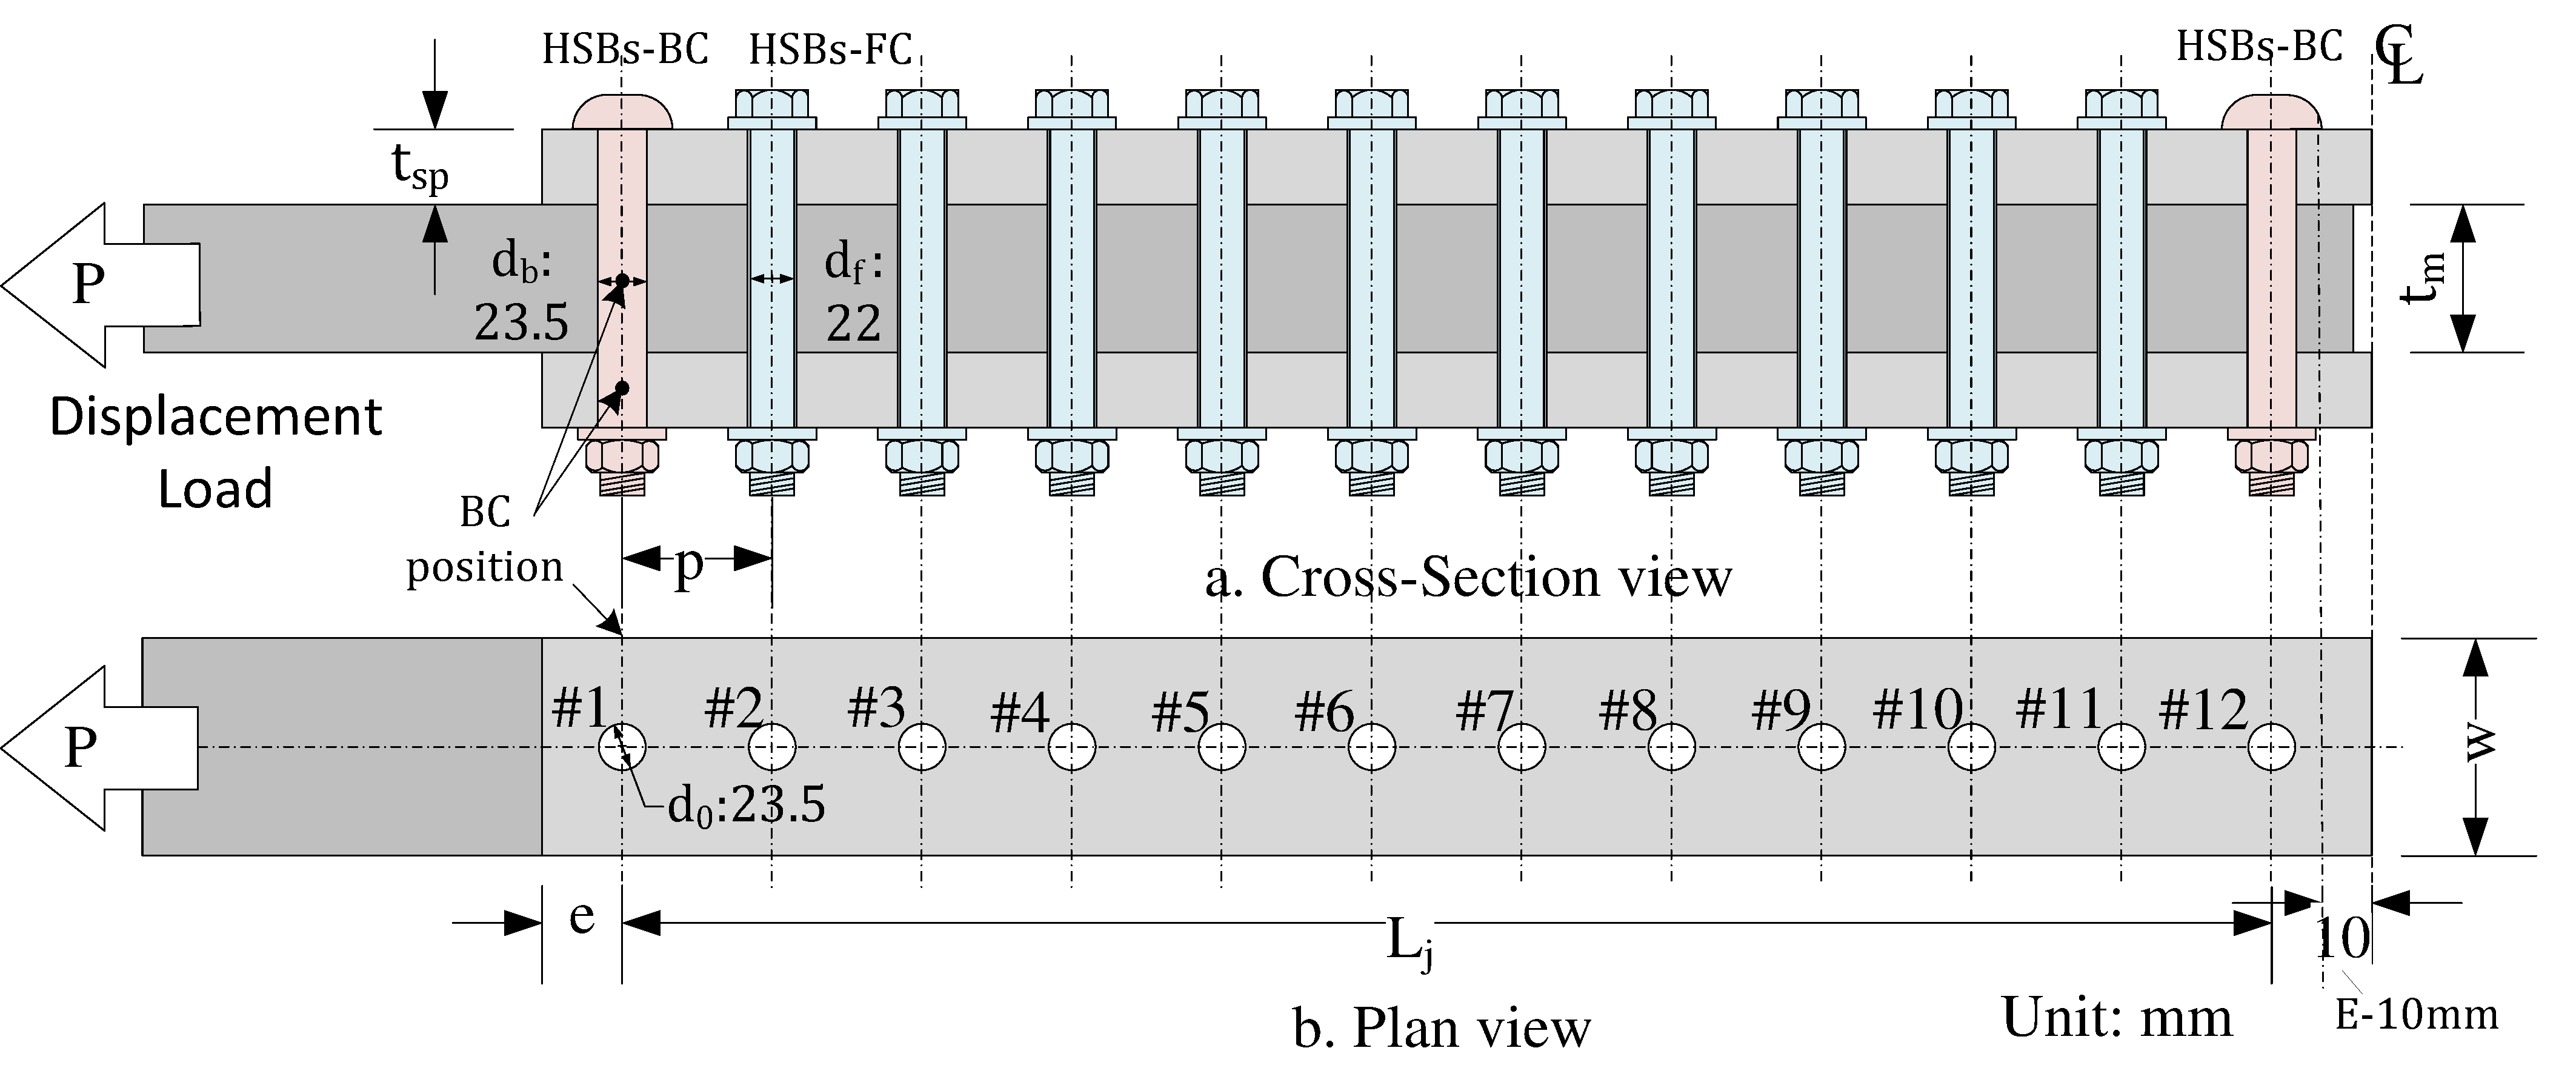
\includegraphics[width=0.95\textwidth]{imgs/ch7/femodelsize.pdf}
    \caption{Schematic illustration of FE model}
    \label{fig8-modelsize}
\end{figure*}

\subsection{Modelling methodology}

A general-purpose structural analysis software, Abaqus / Standard 2020, was utilised to perform a three-dimensional finite displacement elastoplastic analysis \cite{Smith2020}. The analytical model was based on a 12-row bolted friction joint as shown in Figure \ref{fig8-modelsize}, with the bolt arrangement, joint length, plate thickness and material strength as parameters. Displacement load was applied at the end surface of the main plate, and the analysis was conducted for half of the model, with the centre of the joint in the longitudinal direction set as the axis of symmetry. The diameter of the bearing bolt was set as the same as the bolt hole of 23.5 mm, and the diameter of the friction bolt was set as 22 mm.

The modeling method used in this study is based on the previous research \cite{Chen2023MechanicalConnections}, and the results are compared with the experimental results \cite{chen_experimental_2024}. The validity of this analysis is provided in Appendix \ref{sec-valid}.

The material properties and nominal stress - nominal strain curves of the materials used in the analysis are presented in Tables \ref{tab-mateproper} and \ref{fig-matpro}. The material SM490Y and SM570 were used for the main plate and splice plates \cite{JISsteel}, and the high-strength bolts of friction and bearing type (hereinafter known as HSB) had material properties of F10T material \cite{JISbolt} (equivalent to ASTM A490 or Grade 10.9) \cite{ASTM-bolt,ISO-bolt}. All material properties were modelled using a trilinear model with a quadratic gradient of $E/100$, and the ultimate strength was considered.


Figure \ref{fig-femesh} depicts the mesh division of the analytical model. The mesh division and element selection are based on the previous study by Ju. S. H. et al. \cite{ju2004-boltfea}. The mesh size for the main plate was set at 1/15 (5 mm) relative to the plate thickness direction. For the friction-type bolt, the mesh size was set to 2 mm, for the bearing-type bolt to 2.9 mm, for the washer to 3 mm, and for the nut to 5 mm. The Incompatible mode eight-node brick element (C3D8I) was utilized in this model, this element utilizes volume integration, allowing for a more accurate representation of large deformations and complex material behaviour.

Contact boundaries were set between the main plate and splice plates, bolt hole wall and bolt shank, and washer and splice plates to simulate the contact conditions, separation, and fixation. For the contact boundary condition (see Figure \ref{fig-contactp}), the surface-to-surface discretization method was used to avoid surface penetration, while the finite sliding tracking approach allowed for unrestricted movement of the contact surfaces. To simulate boundary non-linearity, hard contact and penalty friction were employed to define the normal and tangential behaviours of the contact pairs, with isotropic Coulomb friction modelling the frictional forces. The friction coefficient of this analysis at the faying surface refers the Japanese Specifications for Highway Bridges (JSHB) set at 0.4 \cite{douji2017,shishin2009}. 

The present analysis refers to previous studies \cite{Kim2007,hung1996,Shimozato2008ExperrimentalModel} to modelling the bolt. Initially, the bolt was tightened to the design bolt preload (205 kN) using the Abaqus option for bolt load, and then it was fixed at its original bolt-shank length in subsequent steps. This approach ensures that the bolt length remains constant, allowing the force in the bolt to vary according to the model's response \cite{Smith2020}. In the next step, forced displacement was applied to the end of the main plate.

\subsection{Analysis case}
To investigate the interaction between friction and bearing in hybrid joints, this study parameterised the arrangement of the bolts, the length of the joint (or number of bolts) and the geometry of the joint, as shown in Table \ref{tab-cases}.

\begin{table}[]
    \centering
\caption{Parameter for FE analysis}
\begin{tabular}{@{}ll@{}}
\toprule
Parameter                   &              \\ \midrule
Number of Row               & 8, 10, 12      \\
Number of Fit bolt          & 0, 2, 4, 6, 8, 12 \\
Material property {[}Mpa{]} & 365, 547     \\
Bolt peach [mm]             & 75, 80, 85     \\
End distance  [mm]          & 35, 40, 50     \\ \bottomrule
\end{tabular}
\label{tab-cases}
\end{table}

\subsection{Calculation of joint resistance}

\begin{table*}[htbp]
\centering
\caption{Detail of analysis case}
\begin{tabular}{@{}llllllllllllllll@{}}
\toprule
code & $w$ & $t_m$ & $t_{sp}$ & $n$ & $n_b$ & $p$ & $e$ & $L_j$ & $f_y$ & $F_s$ & $F_b$ & $F_{h,sh}$ & $F_y$ & $\beta_1$ & $\beta_h$ \\ \midrule
OA0 & 110 & 75 & 38 & 12 & 0 & 75 & 40 & 825 & 365 & 1968 & - & - & 2368 & 0.83 & - \\
OA2 & 110 & 75 & 38 & 12 & 2 & 75 & 40 & 825 & 365 & 1968 & 902 & 2870 & 2368 & 0.83 & 1.23 \\
OA4 & 110 & 75 & 38 & 12 & 4 & 75 & 40 & 825 & 365 & 1968 & 1803 & 3771 & 2368 & 0.83 & 1.6 \\
OA12 & 110 & 75 & 38 & 12 & 12 & 75 & 40 & 825 & 365 & 1968 & 5412 & 5412 & 2368 & 0.83 & 2.28 \\
OAP0 & 110 & 75 & 38 & 12 & 0 & 80 & 50 & 880 & 365 & 1968 & - & - & 2368 & 0.83 & - \\
OAP2 & 110 & 75 & 38 & 12 & 2 & 80 & 50 & 880 & 365 & 1968 & 902 & 2870 & 2368 & 0.83 & 1.23 \\
OAP4 & 110 & 75 & 38 & 12 & 4 & 80 & 50 & 880 & 365 & 1968 & 1803 & 3771 & 2368 & 0.83 & 1.6 \\
OAK0 & 110 & 75 & 38 & 12 & 0 & 80 & 50 & 880 & 365 & 1968 & - & - & 2368 & 0.83 & - \\
OAK2 & 110 & 75 & 38 & 12 & 2 & 80 & 50 & 880 & 365 & 1968 & 902 & 2870 & 2368 & 0.83 & 1.23 \\
OAK4 & 110 & 75 & 38 & 12 & 4 & 80 & 50 & 880 & 365 & 1968 & 1803 & 3771 & 2368 & 0.83 & 1.6 \\
OA2B & 110 & 75 & 38 & 12 & 2 & 75 & 40 & 825 & 547 & 1968 & 902 & 2870 & 3548 & 0.55 & 0.81 \\
OA4B & 110 & 75 & 38 & 12 & 4 & 75 & 40 & 825 & 547 & 1968 & 1803 & 3771 & 3548 & 0.55 & 1.06 \\
OAP2B & 110 & 75 & 38 & 12 & 2 & 80 & 50 & 825 & 547 & 1968 & 902 & 2870 & 3548 & 0.55 & 0.81 \\
OAP4B & 110 & 75 & 38 & 12 & 4 & 80 & 50 & 825 & 547 & 1968 & 1803 & 3771 & 3548 & 0.55 & 1.06 \\
OAK2B & 110 & 75 & 38 & 12 & 2 & 85 & 50 & 825 & 547 & 1968 & 902 & 2870 & 3548 & 0.55 & 0.81 \\
OAK4B & 110 & 75 & 38 & 12 & 4 & 85 & 50 & 825 & 547 & 1968 & 1803 & 3771 & 3548 & 0.55 & 1.06 \\
KA0 & 110 & 75 & 38 & 10 & 0 & 75 & 40 & 675 & 365 & 1640 & - & - & 2368 & 0.69 & - \\
KA2 & 110 & 75 & 38 & 10 & 2 & 75 & 40 & 675 & 365 & 1640 & 902 & 2542 & 2368 & 0.69 & 1.07 \\
KA4 & 110 & 75 & 38 & 10 & 4 & 75 & 40 & 675 & 365 & 1640 & 1803 & 3443 & 2368 & 0.69 & 1.46 \\
KAP2 & 110 & 75 & 38 & 10 & 2 & 80 & 50 & 720 & 365 & 1640 & 902 & 2542 & 2368 & 0.69 & 1.07 \\
KAP4 & 110 & 75 & 38 & 10 & 4 & 80 & 50 & 720 & 365 & 1640 & 1803 & 3443 & 2368 & 0.69 & 1.46 \\
KAK2 & 110 & 75 & 38 & 10 & 2 & 85 & 50 & 765 & 365 & 1640 & 902 & 2542 & 2368 & 0.69 & 1.07 \\
KAK4 & 110 & 75 & 38 & 10 & 4 & 85 & 50 & 765 & 365 & 1640 & 1803 & 3443 & 2368 & 0.69 & 1.46 \\
KA2B & 110 & 75 & 38 & 10 & 2 & 75 & 40 & 675 & 547 & 1640 & 902 & 2542 & 3548 & 0.46 & 0.71 \\
KA4B & 110 & 75 & 38 & 10 & 4 & 75 & 40 & 675 & 547 & 1640 & 1803 & 3443 & 3548 & 0.46 & 0.97 \\
KAK2B & 110 & 75 & 38 & 10 & 2 & 80 & 50 & 720 & 547 & 1640 & 902 & 2542 & 3548 & 0.46 & 0.71 \\
KAK4B & 110 & 75 & 38 & 10 & 4 & 80 & 50 & 720 & 547 & 1640 & 1803 & 3443 & 3548 & 0.46 & 0.97 \\
KAP2B & 110 & 75 & 38 & 10 & 2 & 85 & 50 & 765 & 547 & 1640 & 902 & 2542 & 3548 & 0.46 & 0.71 \\
KAP4B & 110 & 75 & 38 & 10 & 4 & 85 & 50 & 765 & 547 & 1640 & 1803 & 3443 & 3548 & 0.46 & 0.97 \\
HA2 & 110 & 75 & 38 & 8 & 2 & 75 & 40 & 525 & 365 & 1312 & 902 & 2214 & 2368 & 0.55 & 0.94 \\
HA4 & 110 & 75 & 38 & 8 & 4 & 75 & 40 & 525 & 365 & 1312 & 1803 & 3115 & 2368 & 0.55 & 1.3 \\
HAP2 & 110 & 75 & 38 & 8 & 2 & 80 & 50 & 560 & 365 & 1312 & 902 & 2214 & 2368 & 0.55 & 0.94 \\
HAP4 & 110 & 75 & 38 & 8 & 4 & 80 & 50 & 560 & 365 & 1312 & 1803 & 3115 & 2368 & 0.55 & 1.3 \\
HAK2 & 110 & 75 & 38 & 8 & 2 & 85 & 50 & 595 & 365 & 1312 & 902 & 2214 & 2368 & 0.55 & 0.94 \\
HAK4 & 110 & 75 & 38 & 8 & 4 & 85 & 50 & 595 & 365 & 1312 & 1803 & 3115 & 2368 & 0.55 & 1.3 \\
HA2B & 110 & 75 & 38 & 8 & 2 & 75 & 40 & 525 & 547 & 1312 & 902 & 2214 & 3548 & 0.37 & 0.62 \\
HA4B & 110 & 75 & 38 & 8 & 4 & 75 & 40 & 525 & 547 & 1312 & 902 & 3115 & 3548 & 0.37 & 0.88 \\
HAP2B & 110 & 75 & 38 & 8 & 2 & 80 & 50 & 560 & 547 & 1312 & 902 & 2214 & 3548 & 0.37 & 0.62 \\
HAP4B & 110 & 75 & 38 & 8 & 4 & 80 & 50 & 560 & 547 & 1312 & 902 & 3115 & 3548 & 0.37 & 0.88 \\
HAK2B & 110 & 75 & 38 & 8 & 2 & 85 & 50 & 595 & 547 & 1312 & 902 & 2214 & 3548 & 0.37 & 0.62 \\
HAK4B & 110 & 75 & 38 & 8 & 4 & 85 & 50 & 595 & 547 & 1312 & 902 & 3115 & 3548 & 0.37 & 0.88 \\
W2B-M16 & 210 & 50 & 28 & 10 & 2 & 55 & 35 & 495 & 547 & 848 & 418 & 1265 & 5251 & 0.16 & 0.24 \\
W2B-t30 & 210 & 30 & 28 & 10 & 2 & 55 & 35 & 495 & 547 & 848 & 418 & 1265 & 3151 & 0.27 & 0.4 \\
W4B & 210 & 50 & 28 & 10 & 4 & 55 & 35 & 495 & 547 & 848 & 836 & 1684 & 5251 & 0.16 & 0.32 \\
W6B & 210 & 50 & 28 & 10 & 6 & 55 & 35 & 495 & 547 & 848 & 1254 & 2102 & 5251 & 0.16 & 0.4 \\ \bottomrule
\end{tabular}
\label{tab-allcase}
\end{table*}


For hybrid joint, the joint resistance $F_{h}$ \cite{Chen2023MechanicalConnections} is:
\begin{equation} \label{eq-fh}
\begin{aligned}
    F_{h,b} &= (n_f+n_b) F_{s1} + n_b F_{by1} \\
    F_{h,sh} &= (n_f+n_b) F_{s1} + n_b F_{shy1} \\
    F_{h} &= min(F_{h,b}, F_{h,sh})
\end{aligned}    
\end{equation}

Where,

\begin{tabular}{ll}
$\sigma_y$ & the yield strengths of the main plate; \\
$\sigma_u$ & the ultimate strengths of the main plate;\\
$\sigma_{yb}$ & the yield strength of the HSB; \\ 
$\mu$ & the friction coefficient;\\ 
$t$ & the thickness of the main plate; \\ 
$w$ & the width of the main plate; \\
$d_0$ & the hole diameter; \\ 
$d_b$ & the diameter of the bolt; \\ 
$N_0$ & Bolt preload before loading; \\
$N_d$ & the design bolt preload; \\
$m$ & the number of shear planes; \\ 
$n_{f}$ & the number of friction-type bolts; \\ 
$n_b$ & the number of bearing-type bolts.
\end{tabular}


\section{Validation of FE model}
\label{sec-valid}


\begin{figure*}
    \centering
    \begin{subfigure}[b]{0.48\linewidth}
        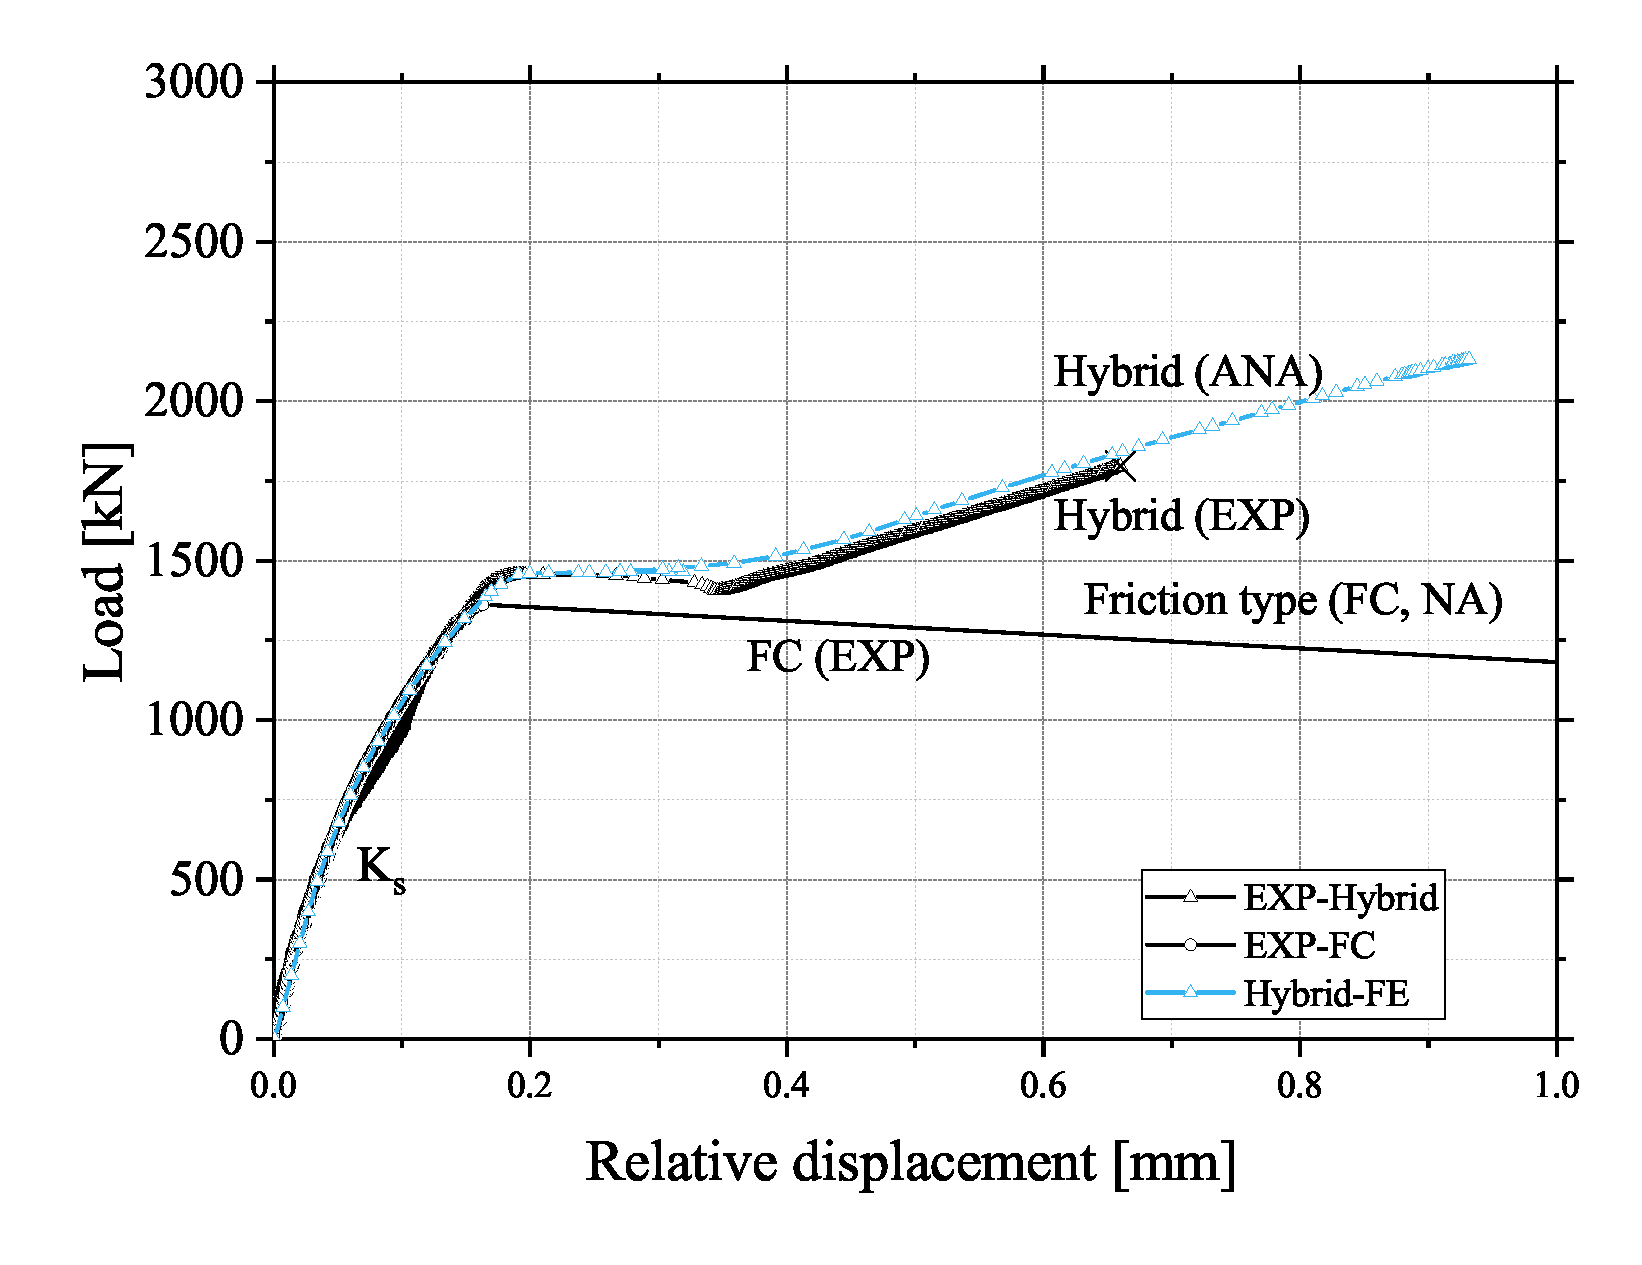
\includegraphics[width=\linewidth]{imgs/ch7/valid-rd.eps}
        \caption{The relationship between load and relative displacement of FE analysis and Experiment result}
        \label{fig-valid-rd}
    \end{subfigure}
    \hfill
    \begin{subfigure}[b]{0.48\linewidth}
    \centering
        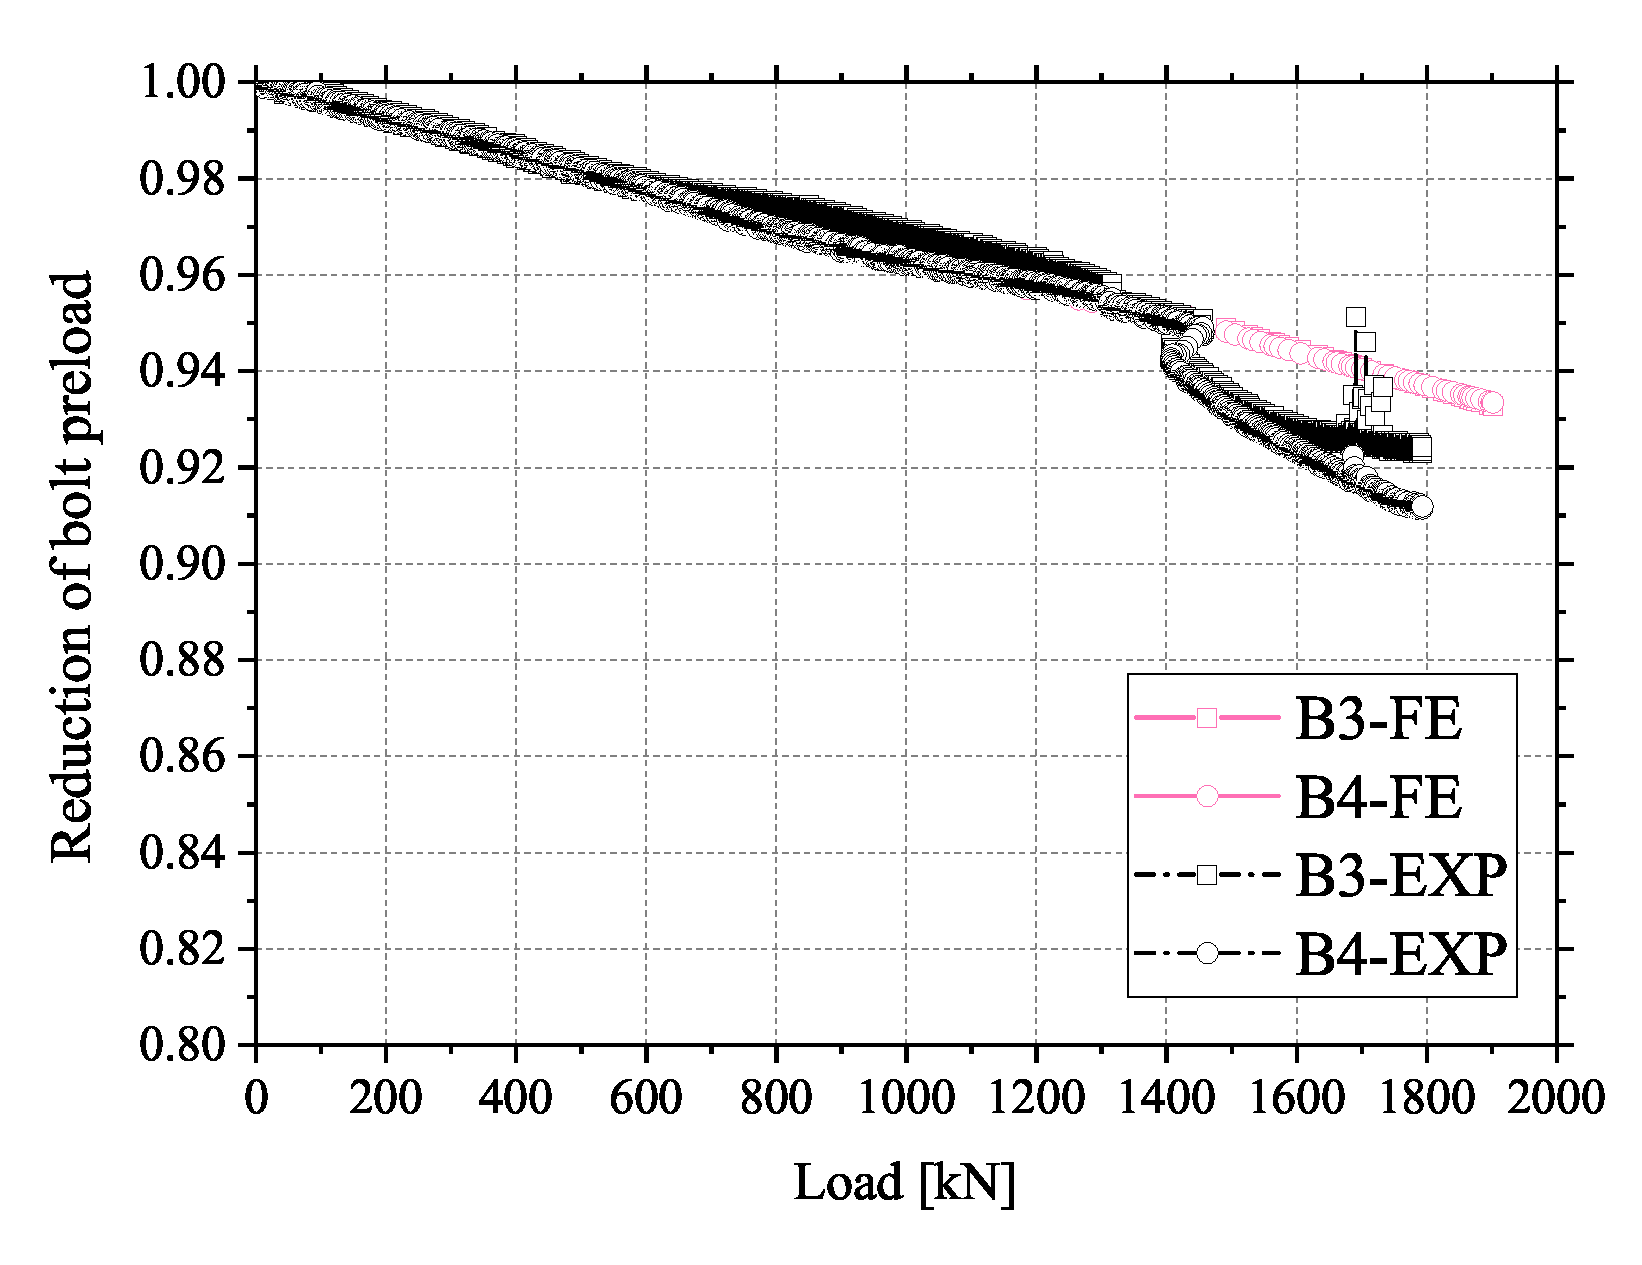
\includegraphics[width=\linewidth]{imgs/ch7/valid-boltAF.eps}
        \caption{The relationship between reduction of bolt preload and load}
        \label{fig-valid-redc}
    \end{subfigure}
    
    \caption{Compare with FE analysis result and experiment result \cite{chen_experimental_2024} }
    \label{fig-valid}
\end{figure*}

The FE analysis model in this paper refers to the Previous study by CHEN et, al. \cite{Chen2023MechanicalConnections} and uses the same modelling method. Additionally, Figure \ref{fig-valid-rd} shows the tensile test results of a full-scale hybrid connection \cite{chen_experimental_2024} and the analysis results of the FE model used in this paper. The blue triangles represent the analytical results, and the black triangles represent the experimental results from previous research. It can be observed that the FE analysis results match well with the experimental results. Figure \ref{fig-valid-redc} shows the bolt preload reduction rates of bolts \# 3 and \# 4 used for friction connection. The pink colour represents the analytical results, and the black colour represents the experimental results measured by the strain gauge. It can be seen that the bolt preload reduction rates in the analysis and experiment results are almost the same. Furthermore, at 1400 kN, the experimental results exhibit a more noticeable change, and the slope of the curve also changes after this point. This is because, in the experiment, due to the failure of friction, the connection experienced a significant slip (the bolts were subjected to a large impact due to the slip), while the analysis is based on static simulation and does not exhibit such dynamic behaviour. Therefore, the load reduction of the bolt axial force appears more gradual in the analysis. It could be considered this analysis method is validity. 

\section{Analysis Results and Discussion}

\subsection{Deformation of hybrid joint}

\begin{figure}[htbp]
    \centering
    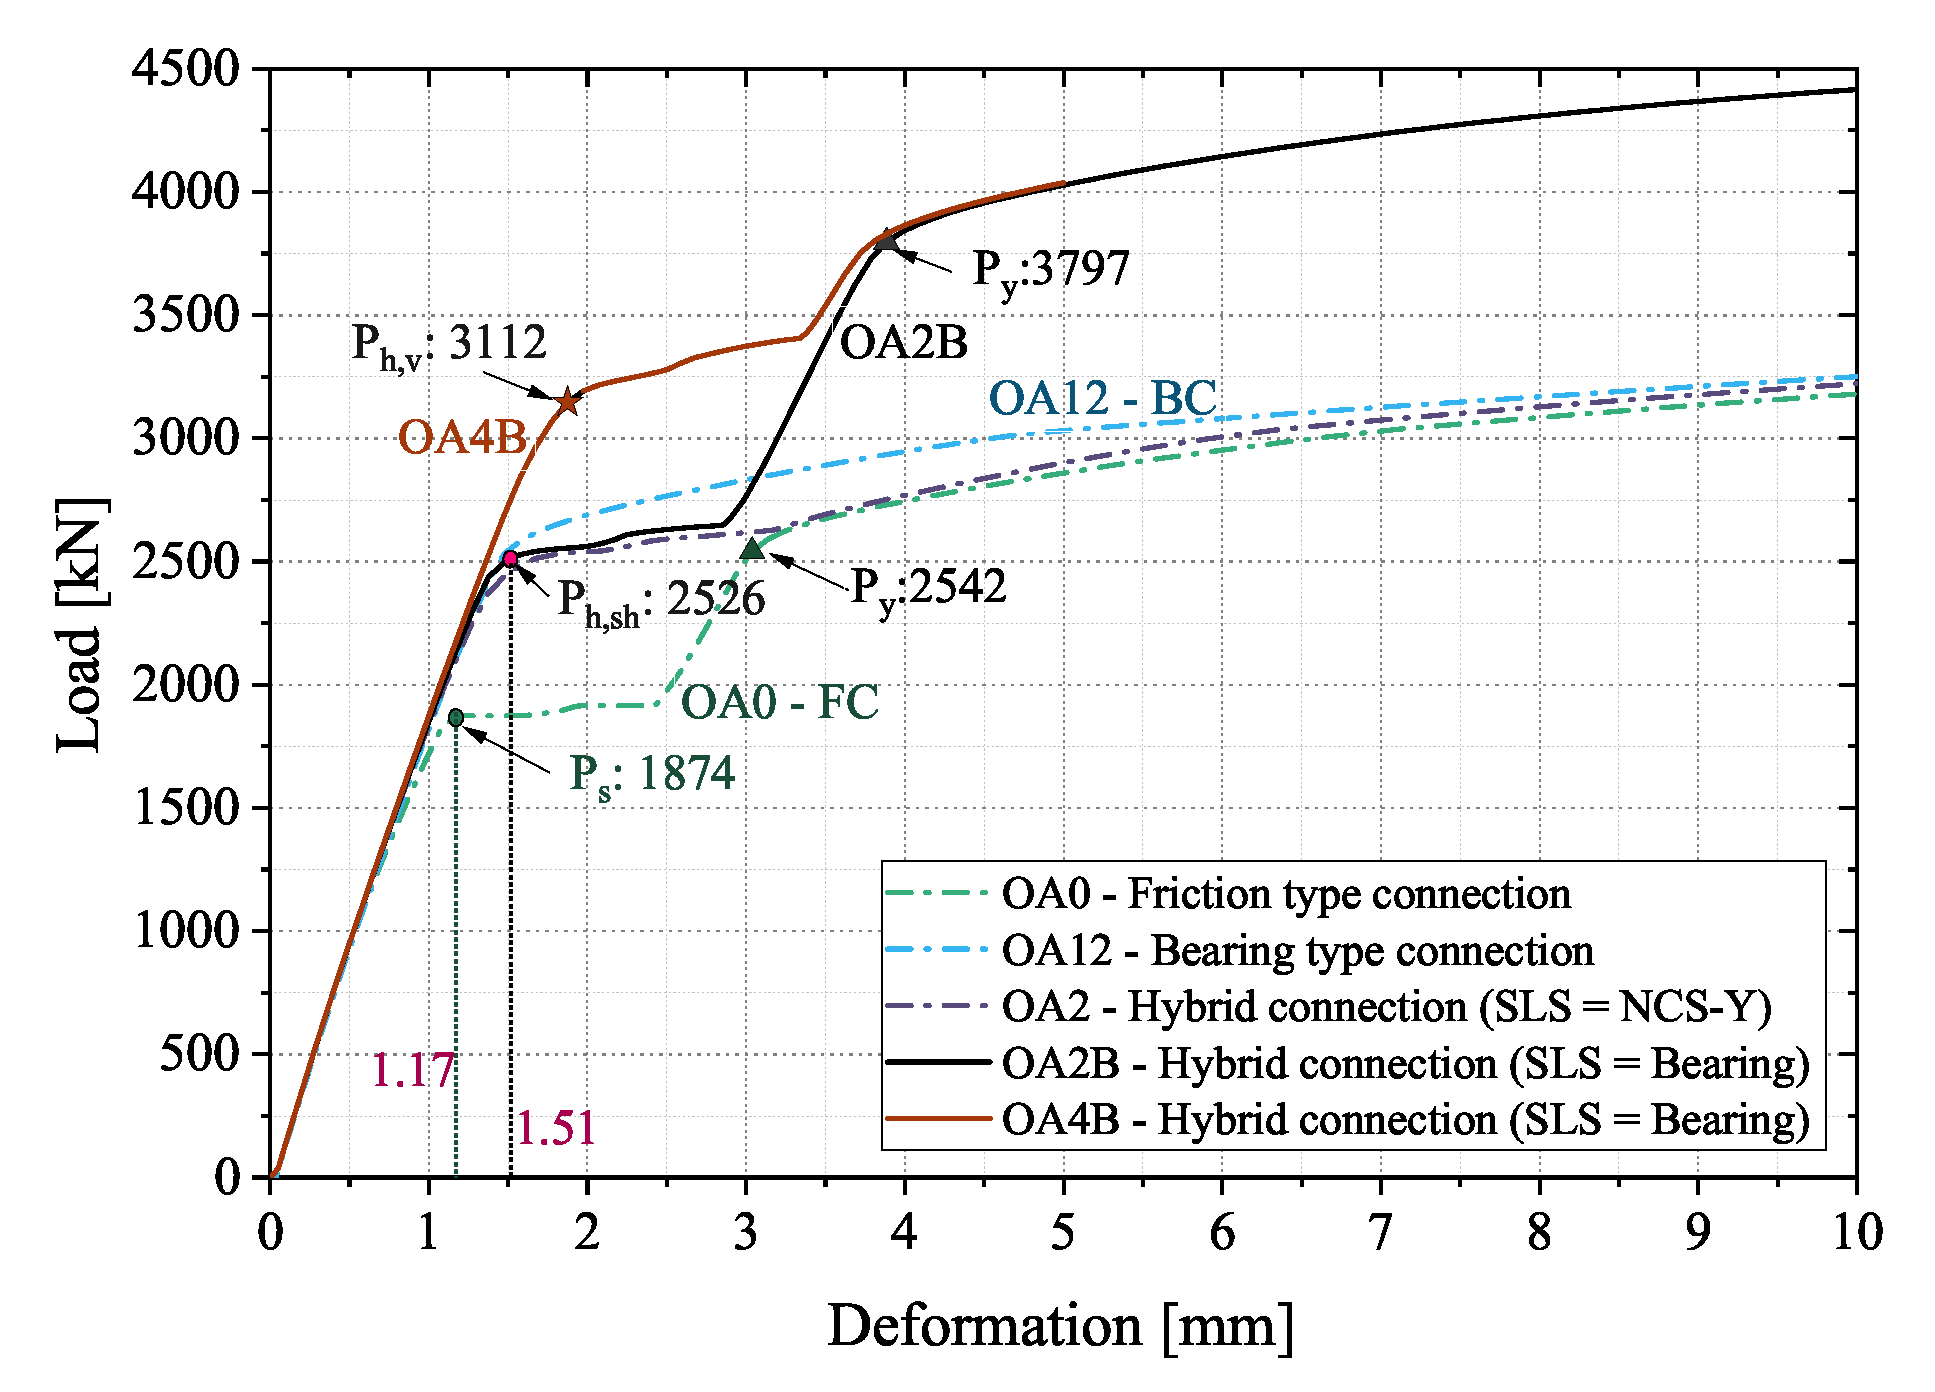
\includegraphics[width=0.7\linewidth]{imgs/ch7/LDef-total.eps}
    \caption{Relationship between the load and deformation}
    \label{fig-ldef}
\end{figure}

\begin{figure}[htbp]
    \centering
    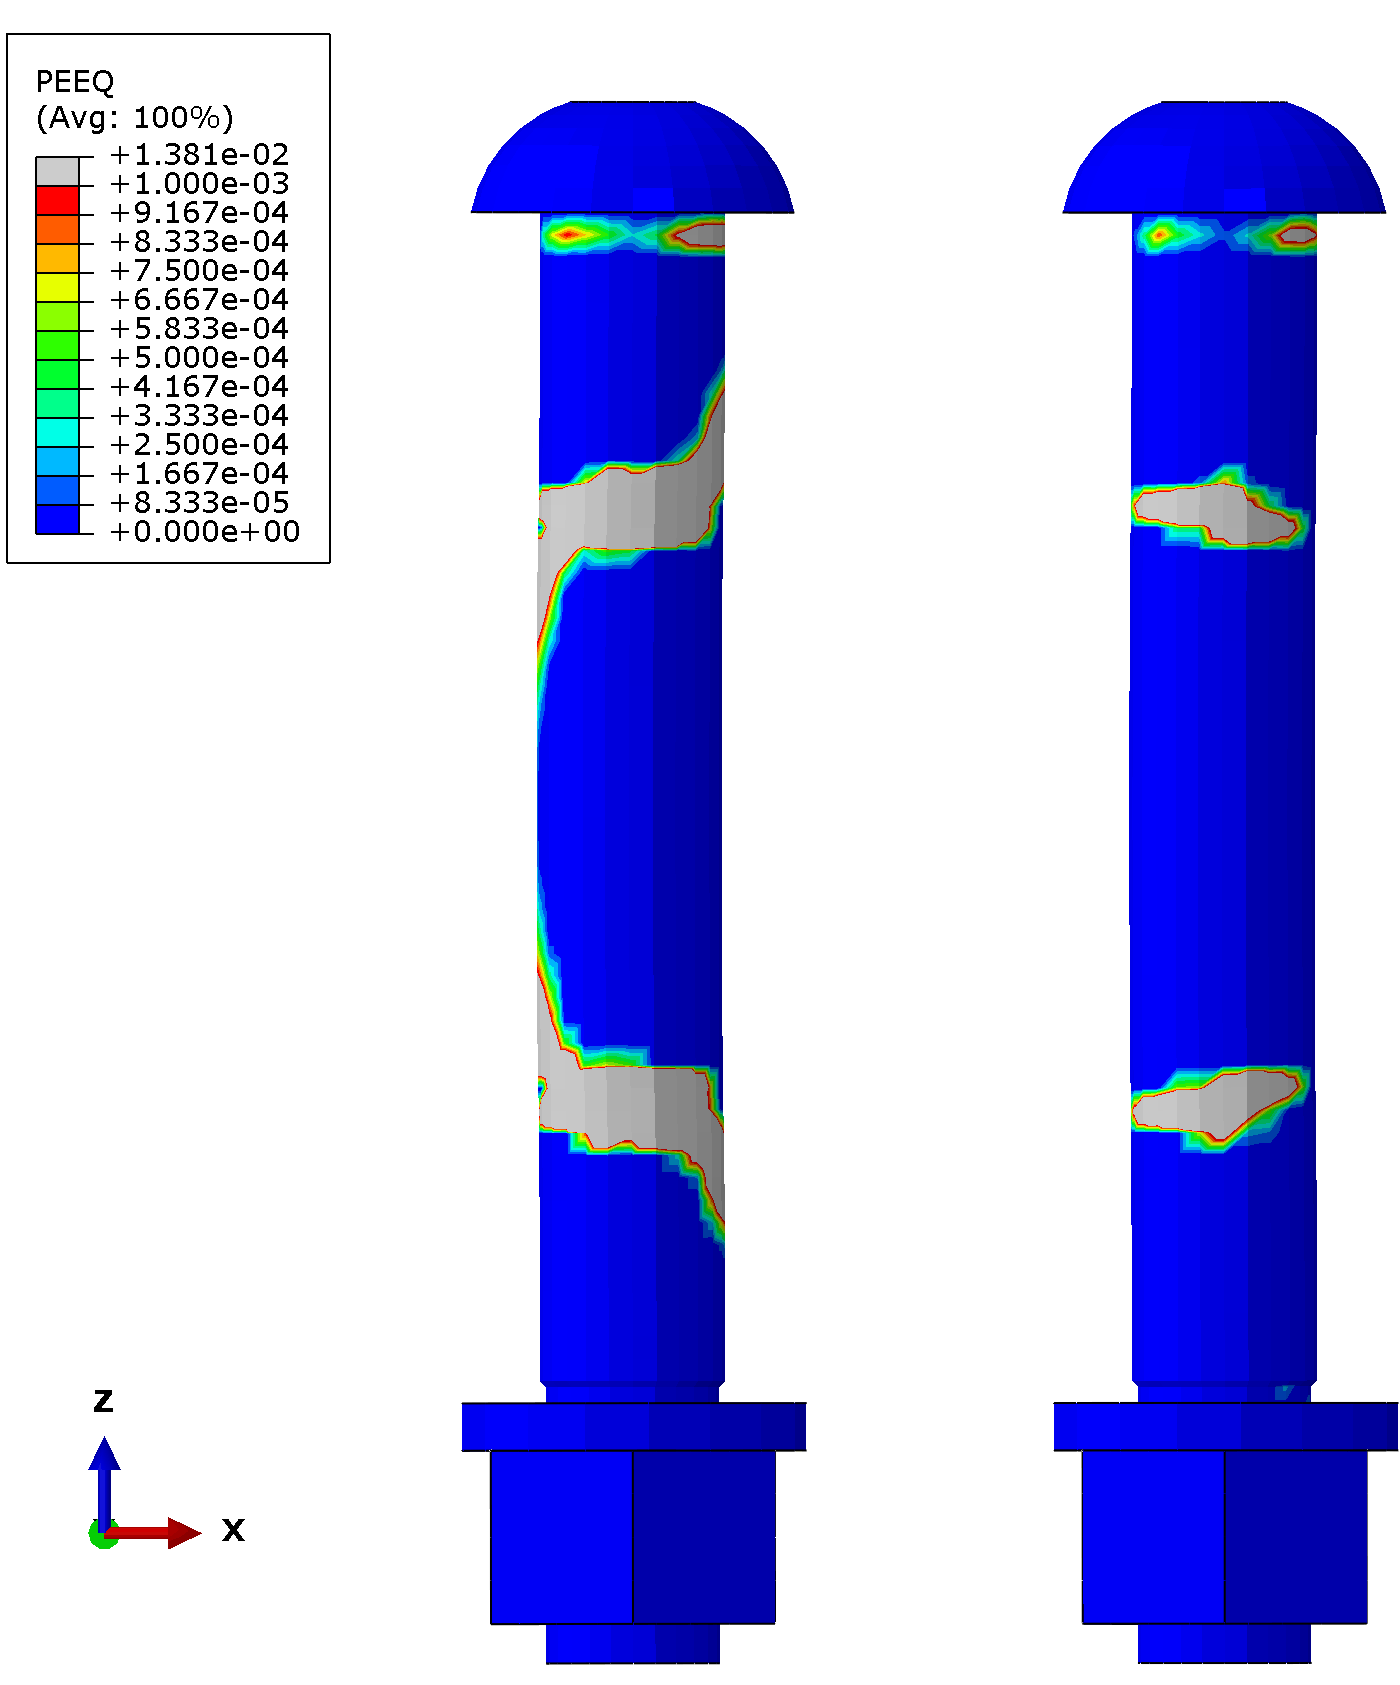
\includegraphics[width=0.5\linewidth]{imgs/ch7/bsh-jud-peeq.png}
    \caption{Judgement of bolt shank shear yield. (PEEQ counter)}
    \label{fig-bsh-jud-peeq}
\end{figure}

Figure \ref{fig-ldef} shows the relationship between the load and deformation. The deformation of the joint was obtained from the average displacement of the cross section at the end of the joint. The OA0 case represents a friction connection, OA12 represents a bearing connection with 12 fit bolts, and OA 2, 2B, and 4B represent hybrid joints. Regardless of the type of connection, the initial stiffness remains the same because it is primarily determined by friction. When the friction connection experienced major slippage, the deformation of the connection was 1.17 mm. For the hybrid joint (OA2B), when bolt shank shear yielding $P_{h,sh}$ occurred, the deformation of the connection was 1.51 mm. The difference was only 0.34 mm. Additionally, after the hybrid joint reached bolt shank shear yielding, the slope of the curve decreased until all the bolts entered the bearing. After the connection was arranged with the fit bolts, the strength of the connection significantly increased (about 35\% at the change point to the nonlinear) and exhibited a curve variation similar to that of the friction connection.

The bolt shank shear yielding $P_{h,sh}$ represents the shear yield resistance of any fit bolt shank in the analysis (defined as the one of SLSs). As shown in Figure \ref{fig-bsh-jud-peeq}, the bolt shank shear yield is defined as an equivalent plastic strain (PEEQ) greater than 0.001 throughout the shear plane.


\subsection{Bearing-friction interaction in load transmission}

\begin{figure*}
\centering
% \begin{subfigure}[b]{0.7\textwidth}
%     \centering
%     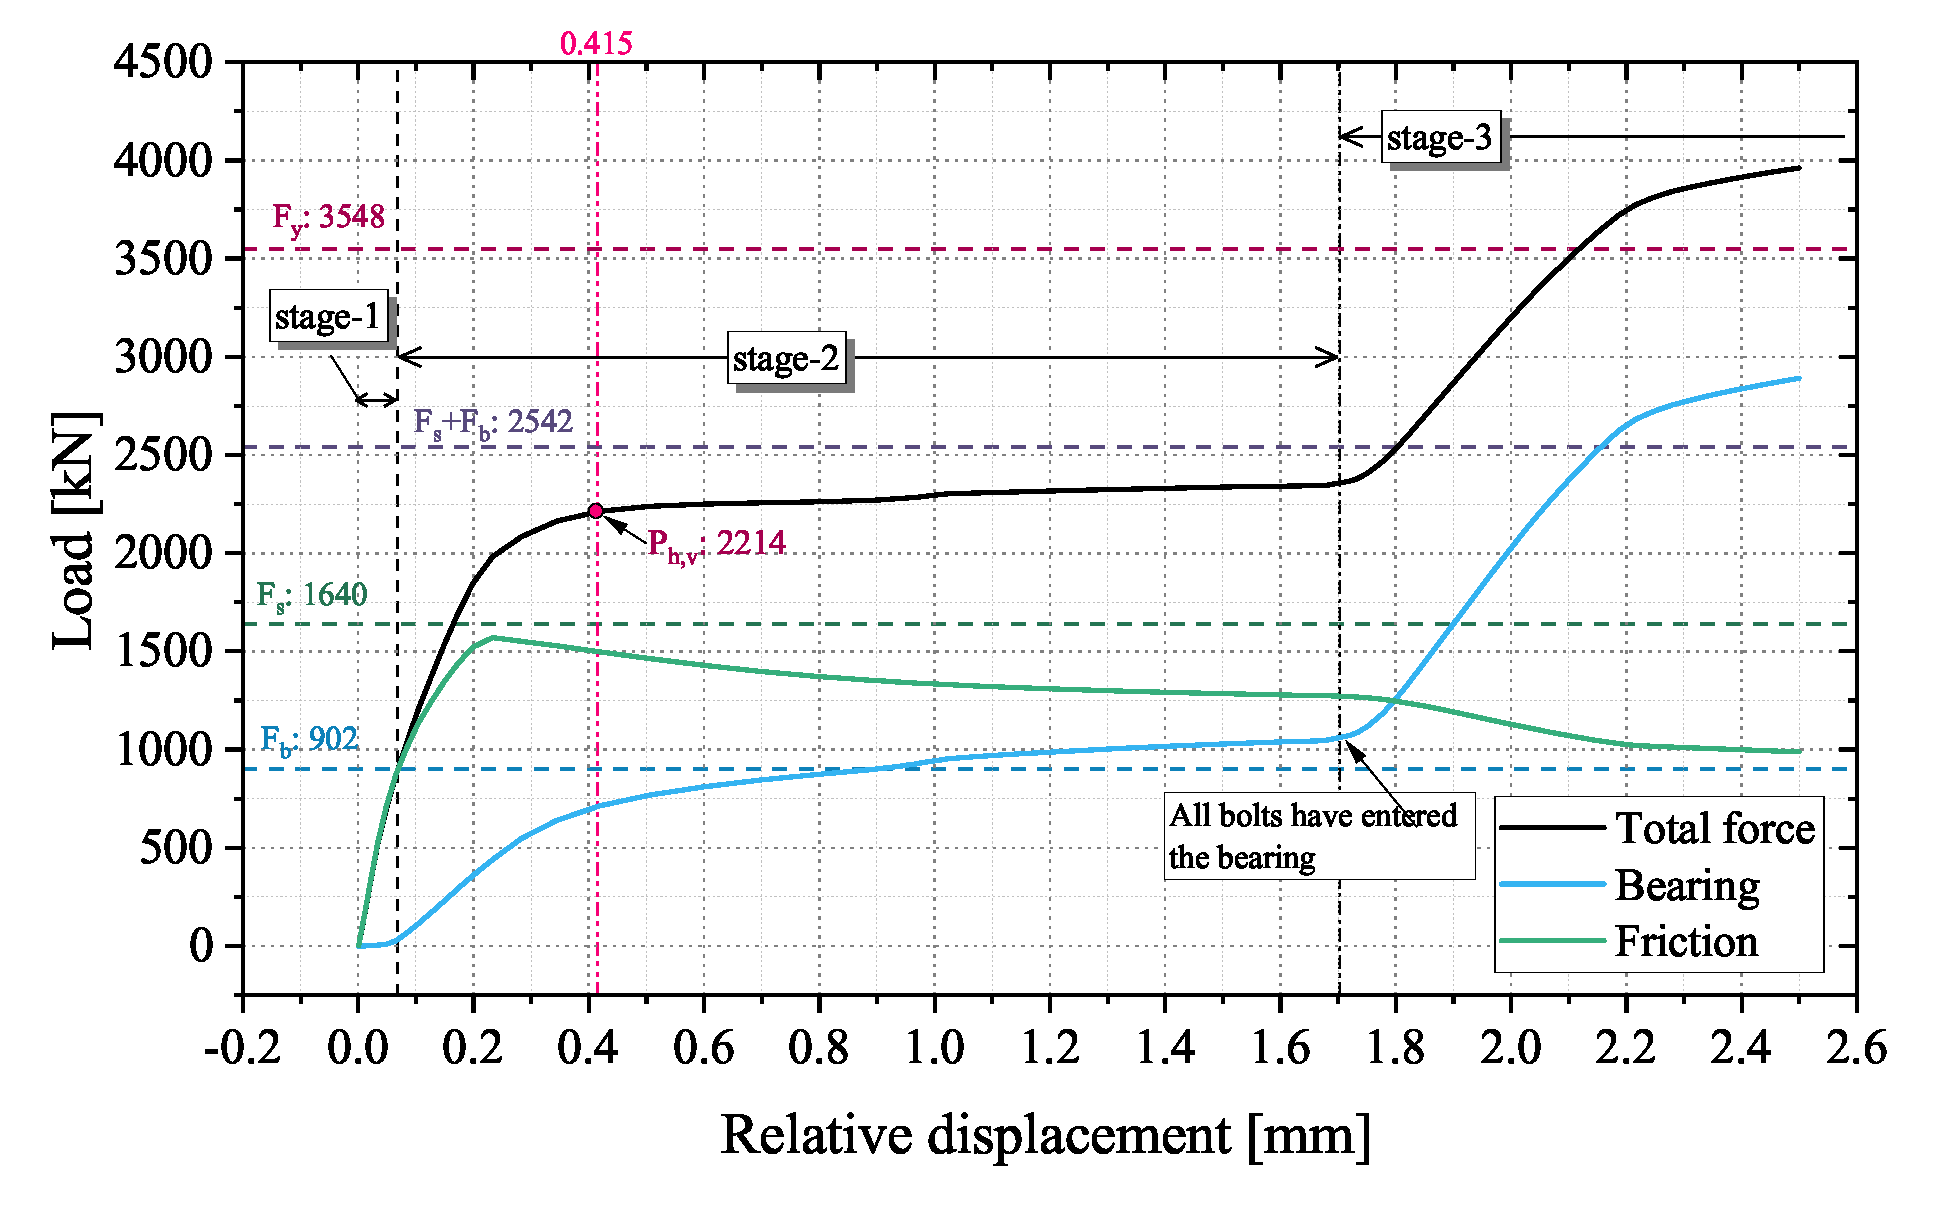
\includegraphics[width=\textwidth]{imgs/ch7/LD-KA2B.eps}
%     \caption{KA2B case}
%     \label{fig-ldka2b}
% \end{subfigure}
% \hfill
% \begin{subfigure}[b]{0.7\textwidth}
%     \centering
%     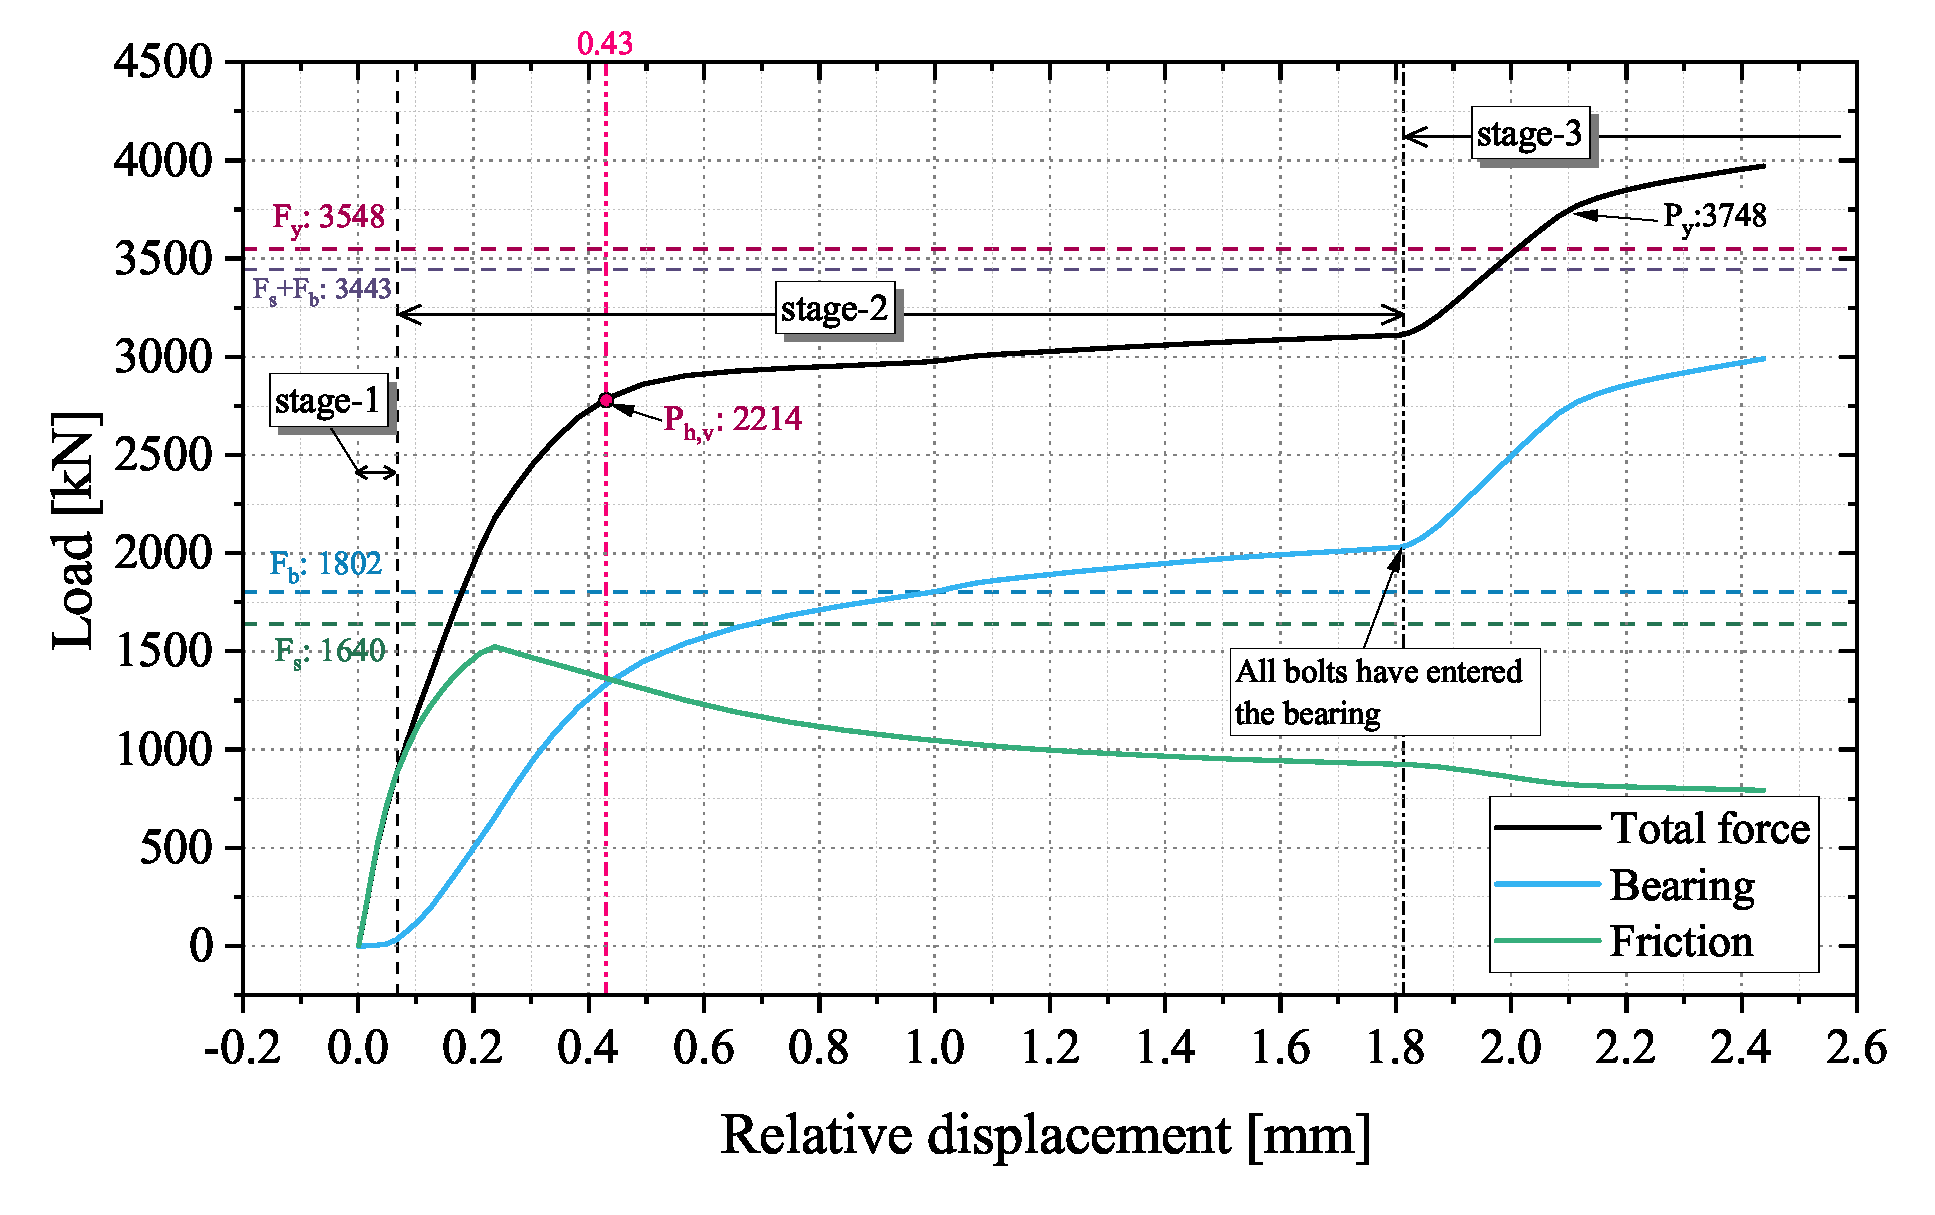
\includegraphics[width=\textwidth]{imgs/ch7/LD-KA4B.eps}
%     \caption{KA4B case}
%     \label{fig-ldka4b}
% \end{subfigure}

\begin{subfigure}[b]{0.85\textwidth}
    \centering
    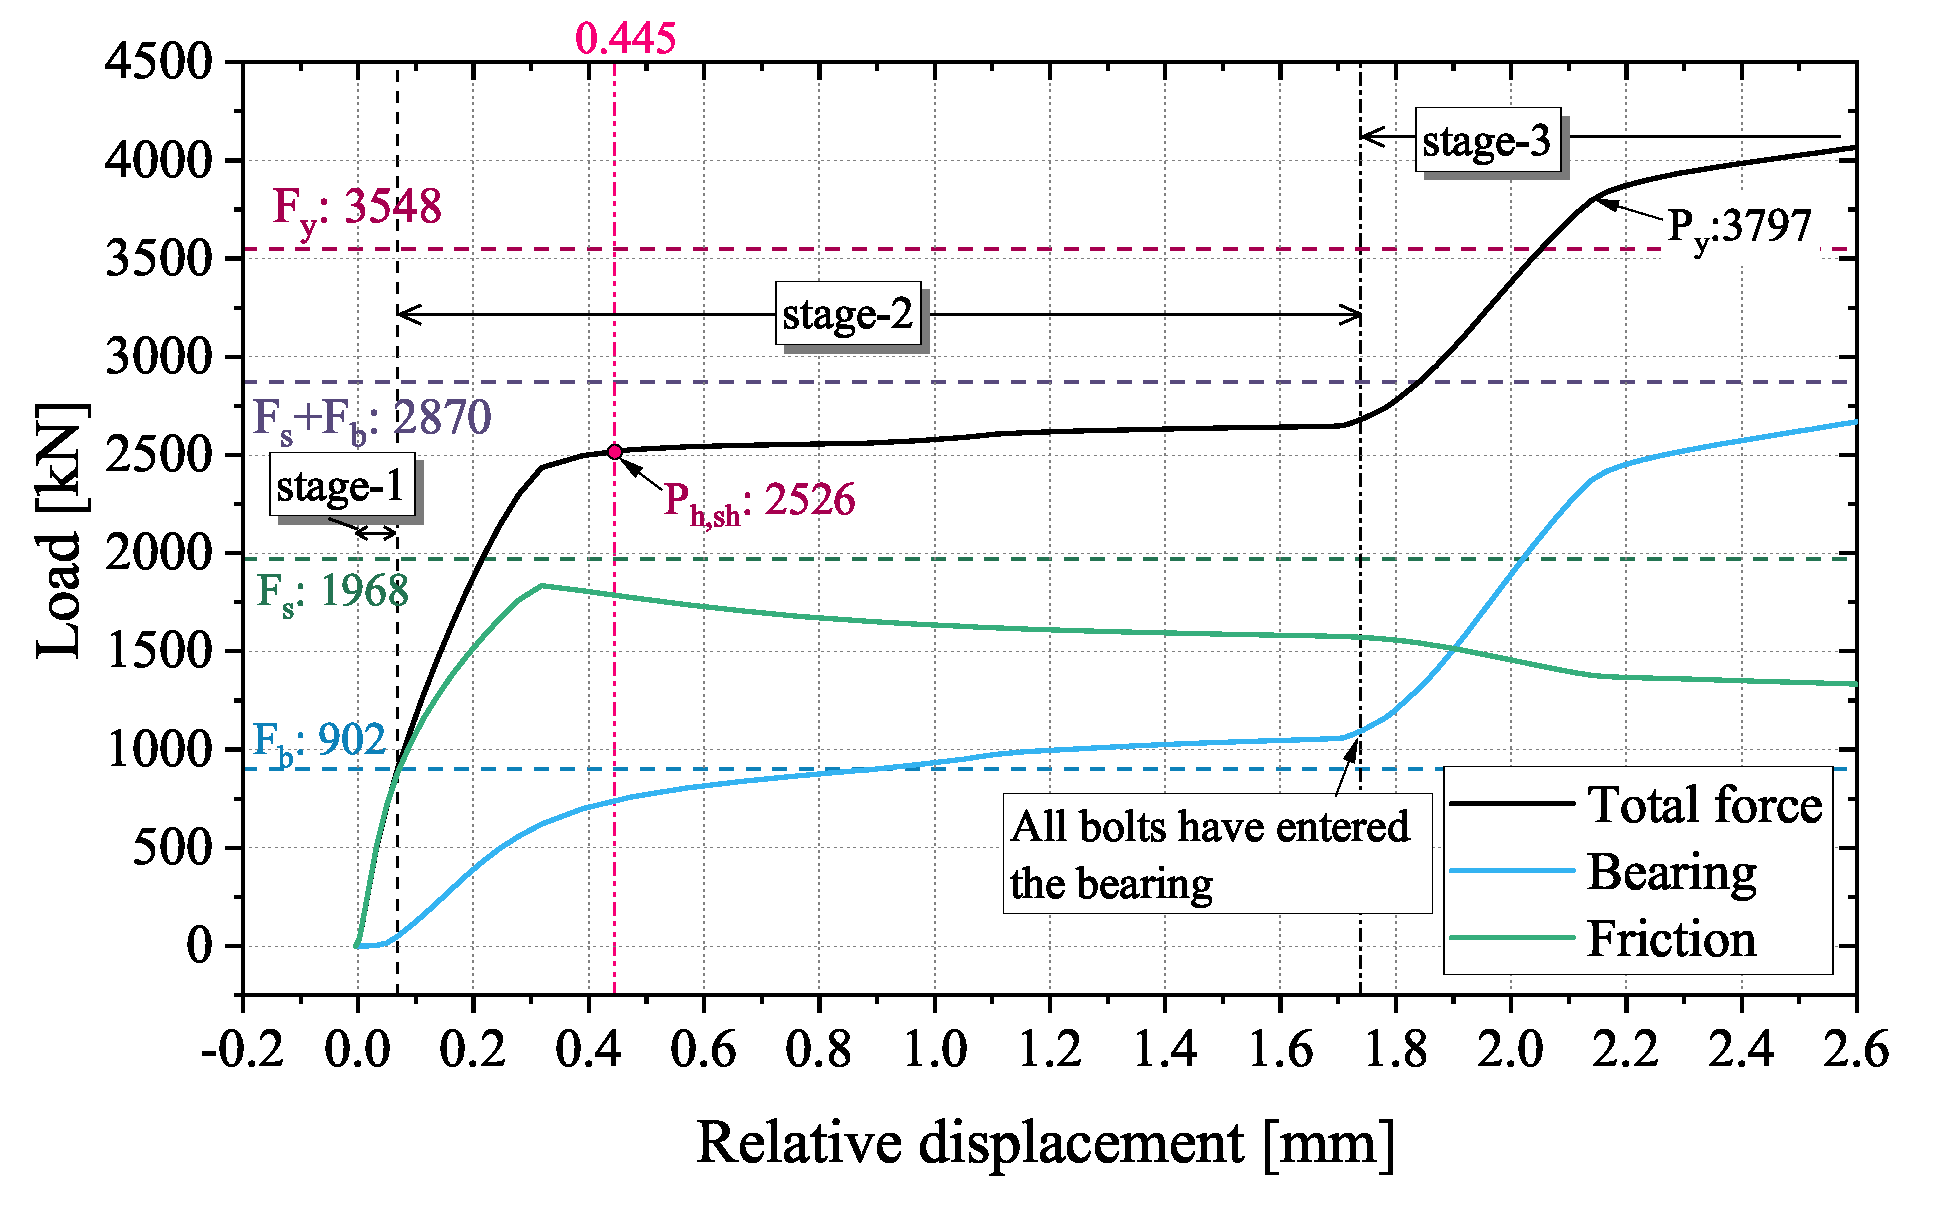
\includegraphics[width=\textwidth]{imgs/ch7/LD-OAP2B.eps}
    \caption{Bolt arrangement: 2/12 ($n_b$ = 2, $n$ = 12), OA2B case, $\beta_h = 0.81$}
    \label{fig-ldoa2b}
\end{subfigure}
\hfill
\begin{subfigure}[b]{0.85\textwidth}
    \centering
    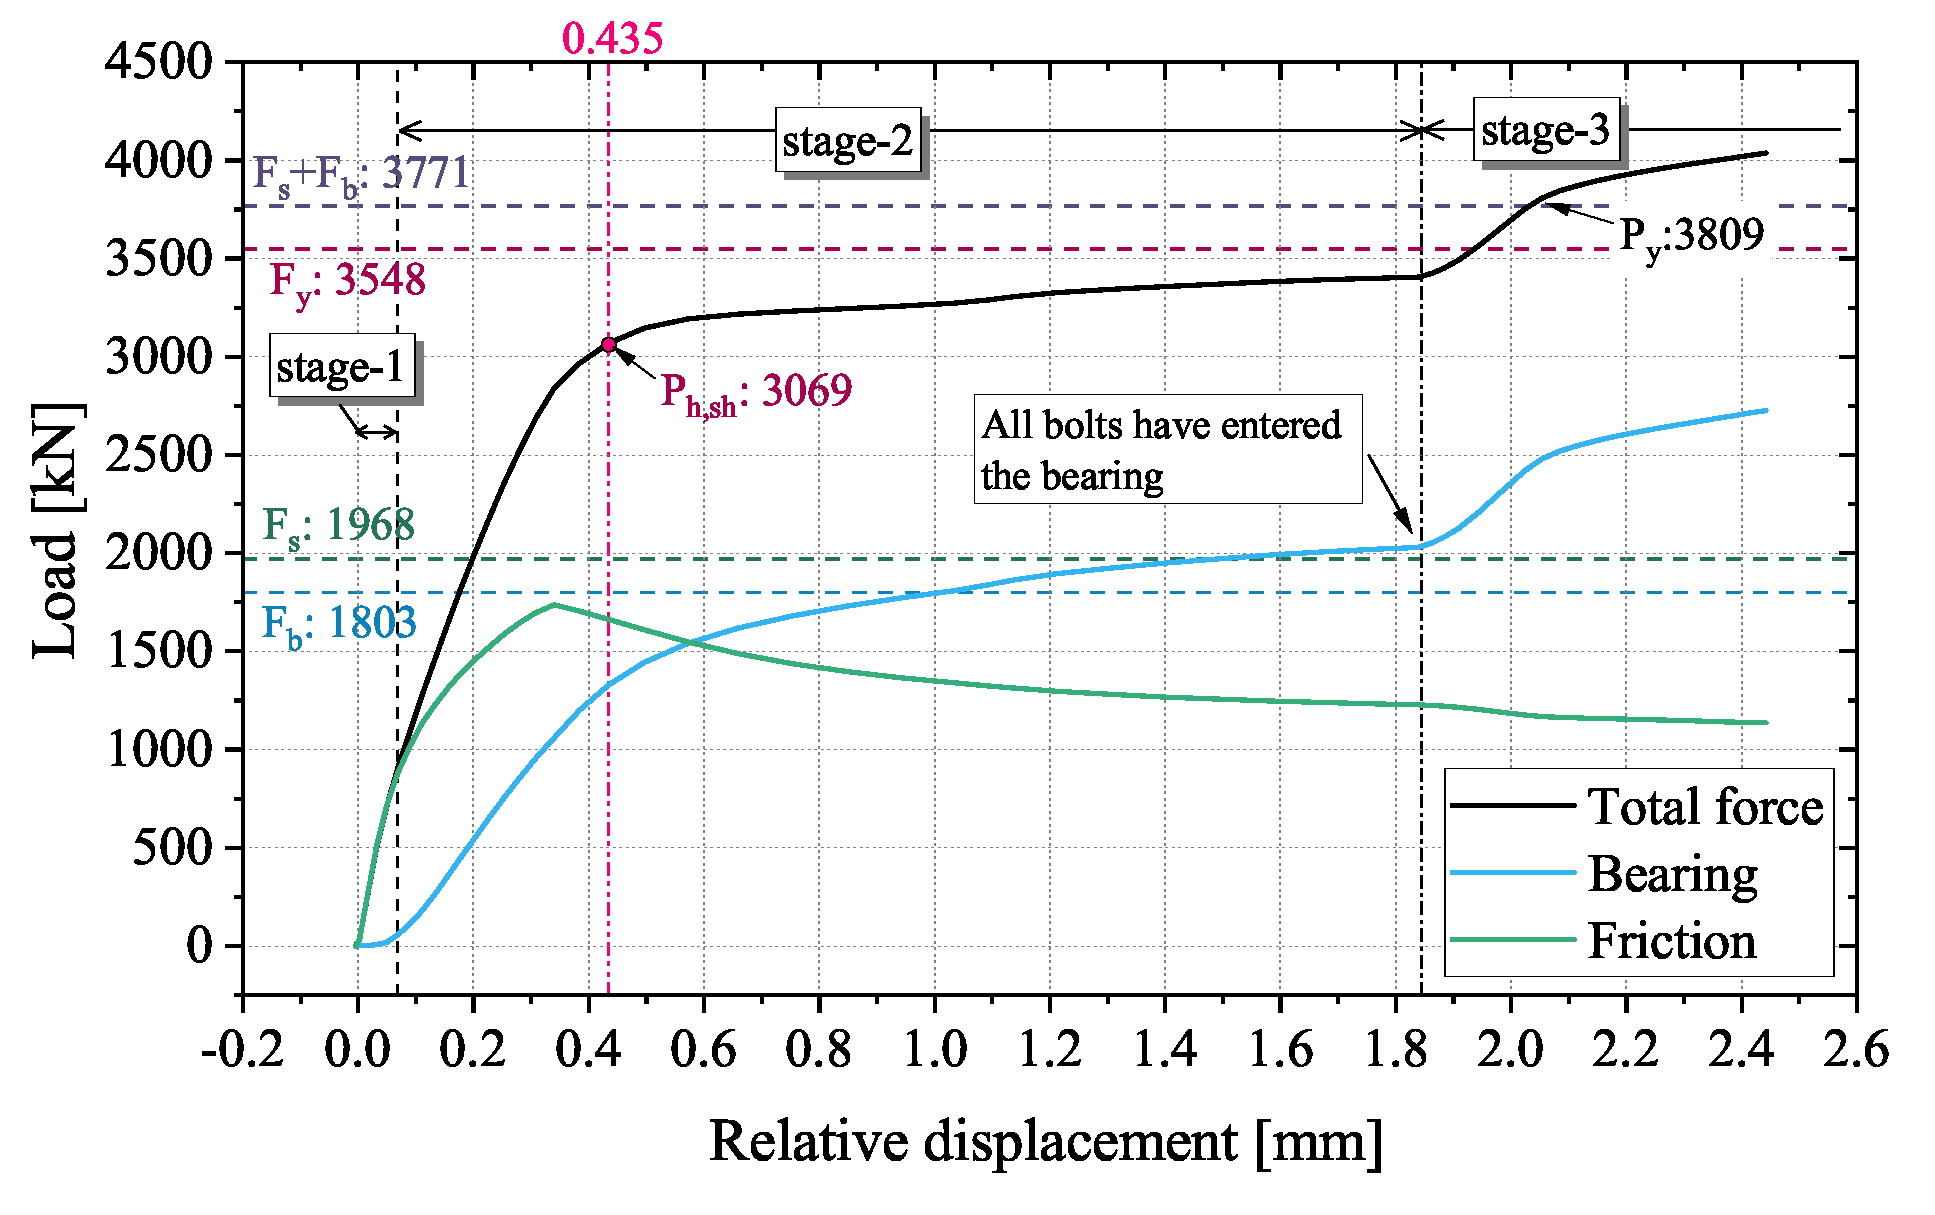
\includegraphics[width=\textwidth]{imgs/ch7/LD-OA4B.eps}
    \caption{Bolt arrangement: 4/12 ($n_b$ = 4, $n$ = 12), OA4B case, $\beta_h = 0.81$}
    \label{fig-ldoa4b}
\end{subfigure}

\caption{Relationship between the relative displacement and load (total force, bearing and friction force), SLSs = Bolt shank shear yield}
\label{fig-loadrd-beaf}
\end{figure*}

Figure \ref{fig-loadrd-beaf} shows the relationship between the relative displacement and the load (total force, bearing and friction force). The relative displacement was referenced from Architectural Institute of Japan (AIJ)'s \cite{AIJ2012AIJStructures} recommendation and taken from a distance of 10 mm from the inner end of the plate. The green dashed line represents the frictional strength $F_s$ calculated using Eq. \ref{eq-fds}, and the blue dashed line represents the bearing strength $F_b$ calculated using Eq. \ref{eq-fdb1}. The red dashed line represents the net section yield strength $F_y$, and the purple dashed line represents the cumulative values of the compressive and frictional strengths ($F_s+F_b$).

As shown in Figure \ref{fig-how2cal-fbfs}, the total force is taken from the integral force at the end of the main plate. The friction force was calculated using the shear stress of the faying surface in the main plate, and the bearing force was the integration of the contact pressures of the hole surfaces.

Figure \ref{fig-loadrd-beaf} shows that whether the case is arranged with two fit bolts (2/12) or with four fit bolts (4/12), bearing connections barely transmit the load at the initial stage. This is due to the friction connection has a much higher stiffness than the bearing connection, and bearing connections hardly transmits the load until a certain amount of elastic slip occurs \cite{fisher1965behavior,Chen2023MechanicalConnections,chen_experimental_2024}. 

In this study, the moment when load sharing begins in bearing connections (i.e., the transfer load combined with friction) is defined as Stage 1. The stiffness of the total force of the joint is almost determined by the stiffness of the friction connection until Stage 1 is reached, after which the stiffness of the total force almost constant, although the bearing connection also starts to transmit loads. The transmission of loads from the friction connection to the hybrid transmission stage of friction and bearing is very gentle. 

After Stage 1, as the load increased, the friction connection reached its maximum resistance, and the slope of the relative displacement curve of the joint decreased. Subsequently, the load continued to be transmitted mainly in a bearing. No significant slippage was observed, as confirmed by the results of the experiment \cite{chen_experimental_2024} shown in Appendix \ref{sec-valid}. Where, all the bolts were in the bearing state, which is called the hybrid load transfer stage (Stage 2).

Notably, in the theoretical of the coulomb friction used for contact pairs, the friction did not decrease even when the maximum value was reached; however, owing to the out-of-plane deformation of the splice plate, shear bending of the bolts, and other factors, the friction force decreased significantly, which will be explained in more detail in Section \ref{sec-decoff}.

The mechanical behaviour and ultimate limit state of the hybrid connection after all the bolts have entered the bearing state (bearing failure mode) can be approximated as a bearing-type bolted connection, which is Stage 3 of the hybrid connection.

In the case of the SLS is bolt shank shear yield, the hybrid joints with two and four fit bolts (see Figure \ref{fig-loadrd-beaf}) produce almost the same relative displacements of approximately 0.43 mm when the bolt shank shear yield strength $P_{h,sh}$ is reached. This is due to the amount of elastic deformation generated when the bolts yield in the shear plane; therefore, if the judgement condition is the load at the shear yield strength of the bolt shank, the amount of elastic deformation generated by that bolt can be assumed to be the same. Therefore, it can be considered that when the hybrid joint reaches the bolt shank shear yield strength $P_{h,sh}$, the end position of the joint will produce a relative displacement of approximately 0.4 mm (The elastic deformation of the steel is ignored).


Figure \ref{fig-lrd-ncy} shows the relative displacement curve of the hybrid connection when the SLS is determined as the net cross-sectional yield. Even when the net cross-section yield is considered the SLS, the hybrid connection can still be divided into three load-transfer stages. The slight difference is that, owing to the tensile deformation of the net cross section, the load that can be transferred by the bearing decreases, and before reaching the net cross-section yielding, both the stiffness of the friction and bearing show a noticeable decreasing trend.



\begin{figure*}
    \centering
    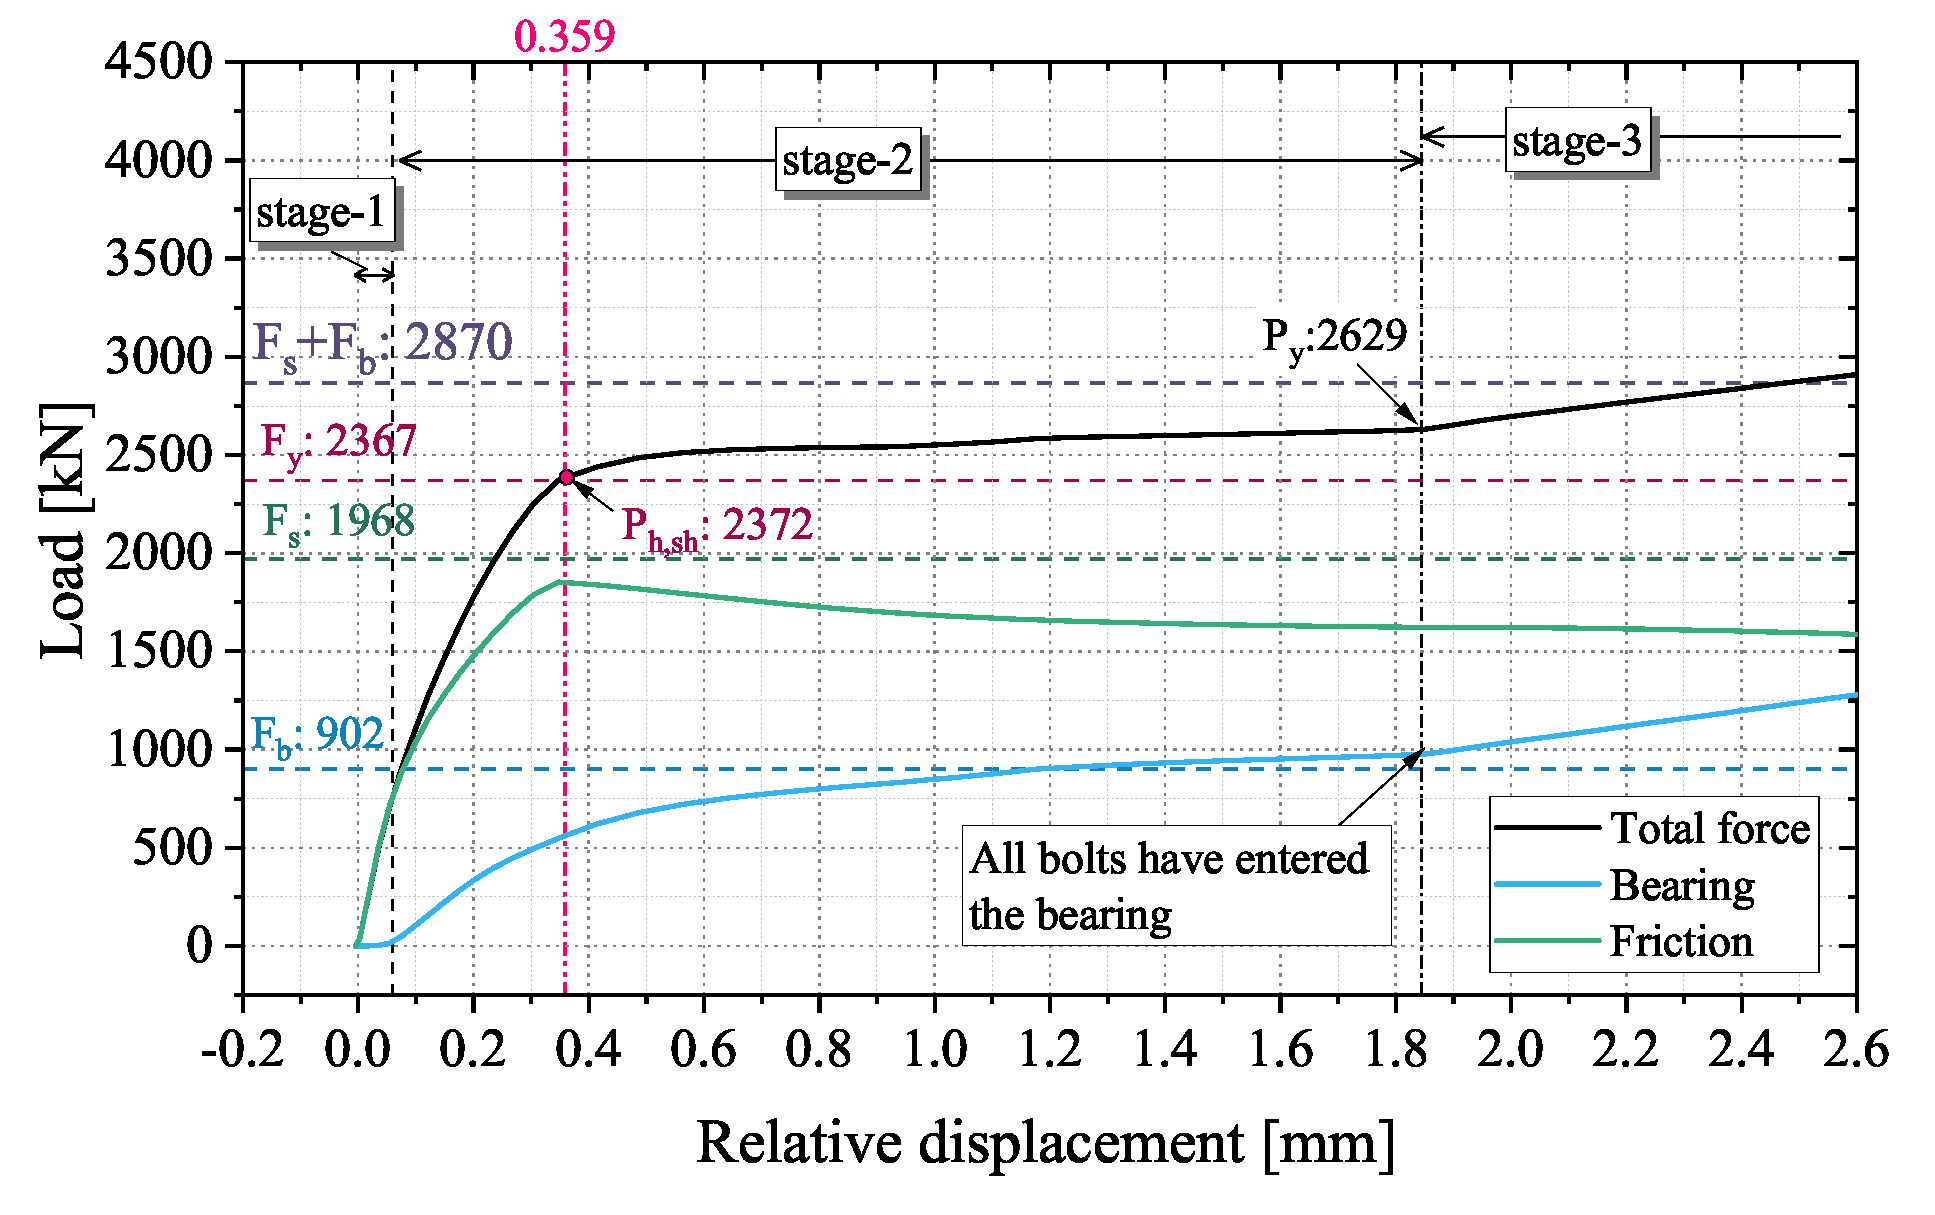
\includegraphics[width=0.85\linewidth]{imgs/ch7/LD-OAP2.eps}
    \caption{Relationship between the relative displacement and load (total, bearing, and friction force), OA2 case (2/12), SLS = Net cross-section yield}
    \label{fig-lrd-ncy}
\end{figure*}


\begin{figure*}
    \centering
    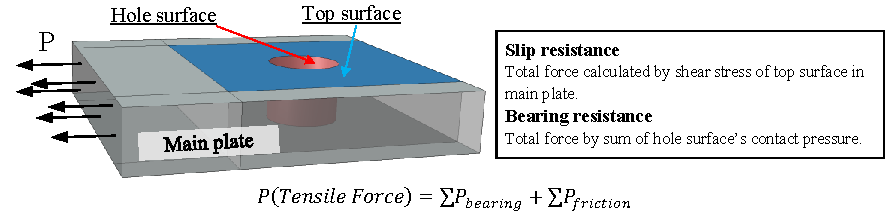
\includegraphics[width=0.85\linewidth]{imgs/ch7/how2cal-fbfs.pdf}
    \caption{Calculation methods of bearing and friction forces}
    \label{fig-how2cal-fbfs}
\end{figure*}

\subsection{Relative displacement of long bolted joint}

Figure \ref{rd-distri} shows the relative displacement distribution at various locations of the hybrid joint (taking the OA4B case as an example), where BC represents the bolt centre location and E-10 mm represents the location 10 mm away from the inner side of the joint. The relative displacement distribution of the connection is nonuniform. When the connection reaches bolt shear yielding in the bolt shank (at SLS), the relative displacement at E-10 mm is 0.43 mm as shown in Figure \ref{fig-modelsize}. The relative displacement becomes smaller towards the middle of the joint, with only 0.12 mm at the locations of bolts \# 6 and \# 7 (BC-6, -7).

The overall average relative displacement of the connection is 0.24 mm, with a median value of only 0.2 mm. The JSHB \cite{douji2017} specifies a relative displacement of 0.2 mm when conducting slip coefficient tests on two rows of friction-type connections. However, for bearing connections, owing to their low stiffness, there is no explicit specification for the relative displacement (allowable slip value). Therefore, with a median relative displacement of only 0.2 mm, the relative displacement of the hybrid connection is well within the acceptable range.


\begin{figure}[htbp]
\centering
    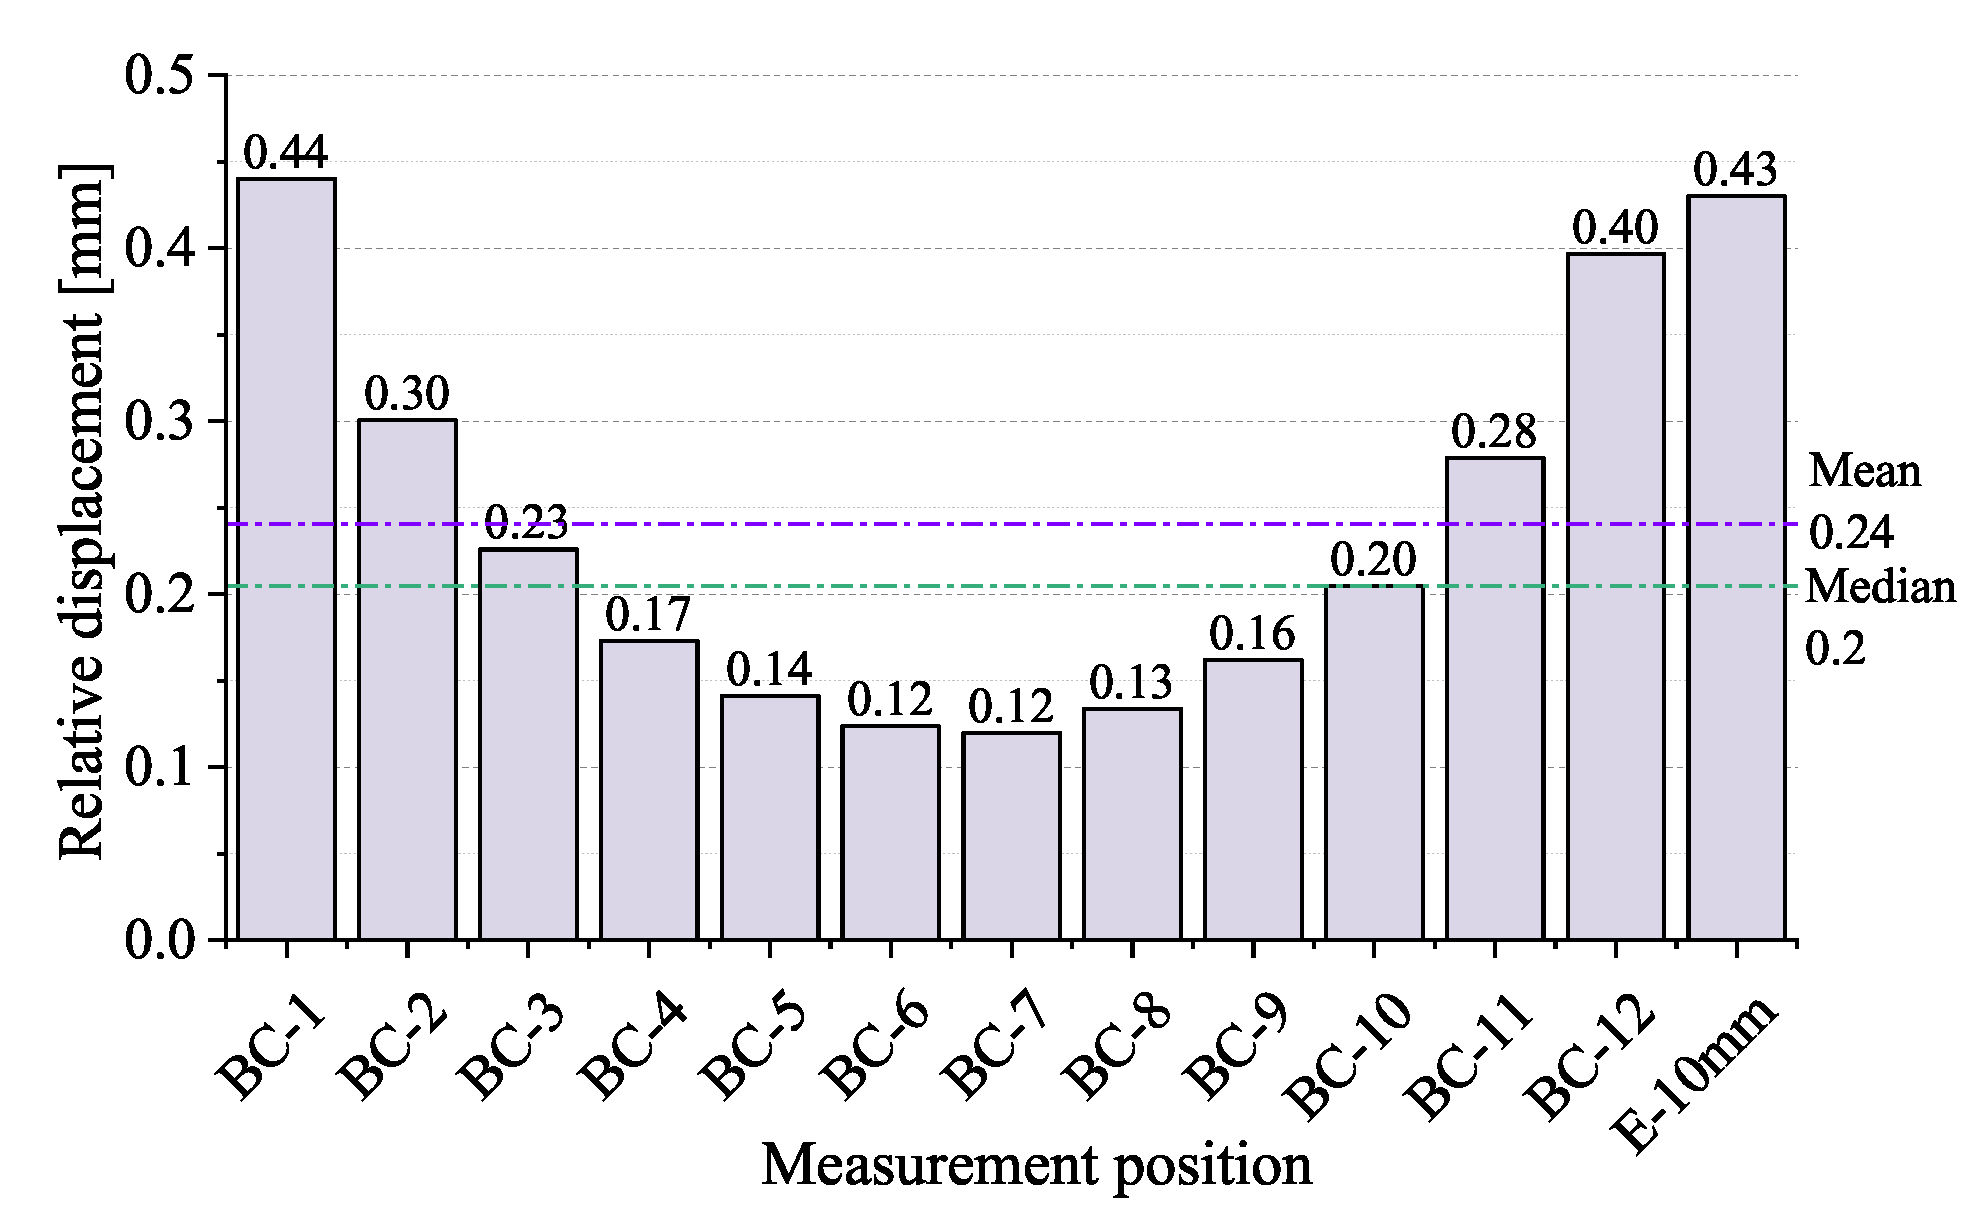
\includegraphics[width=0.7\linewidth]{imgs/ch7/RD-distri-oa4b.eps}
    \caption{Relative displacement of each measurement position in the hybrid joint (OA4B case)}
    \label{rd-distri}
\end{figure}


\subsection{Load sharing of each bolt}
\label{LS}

\begin{figure*}
    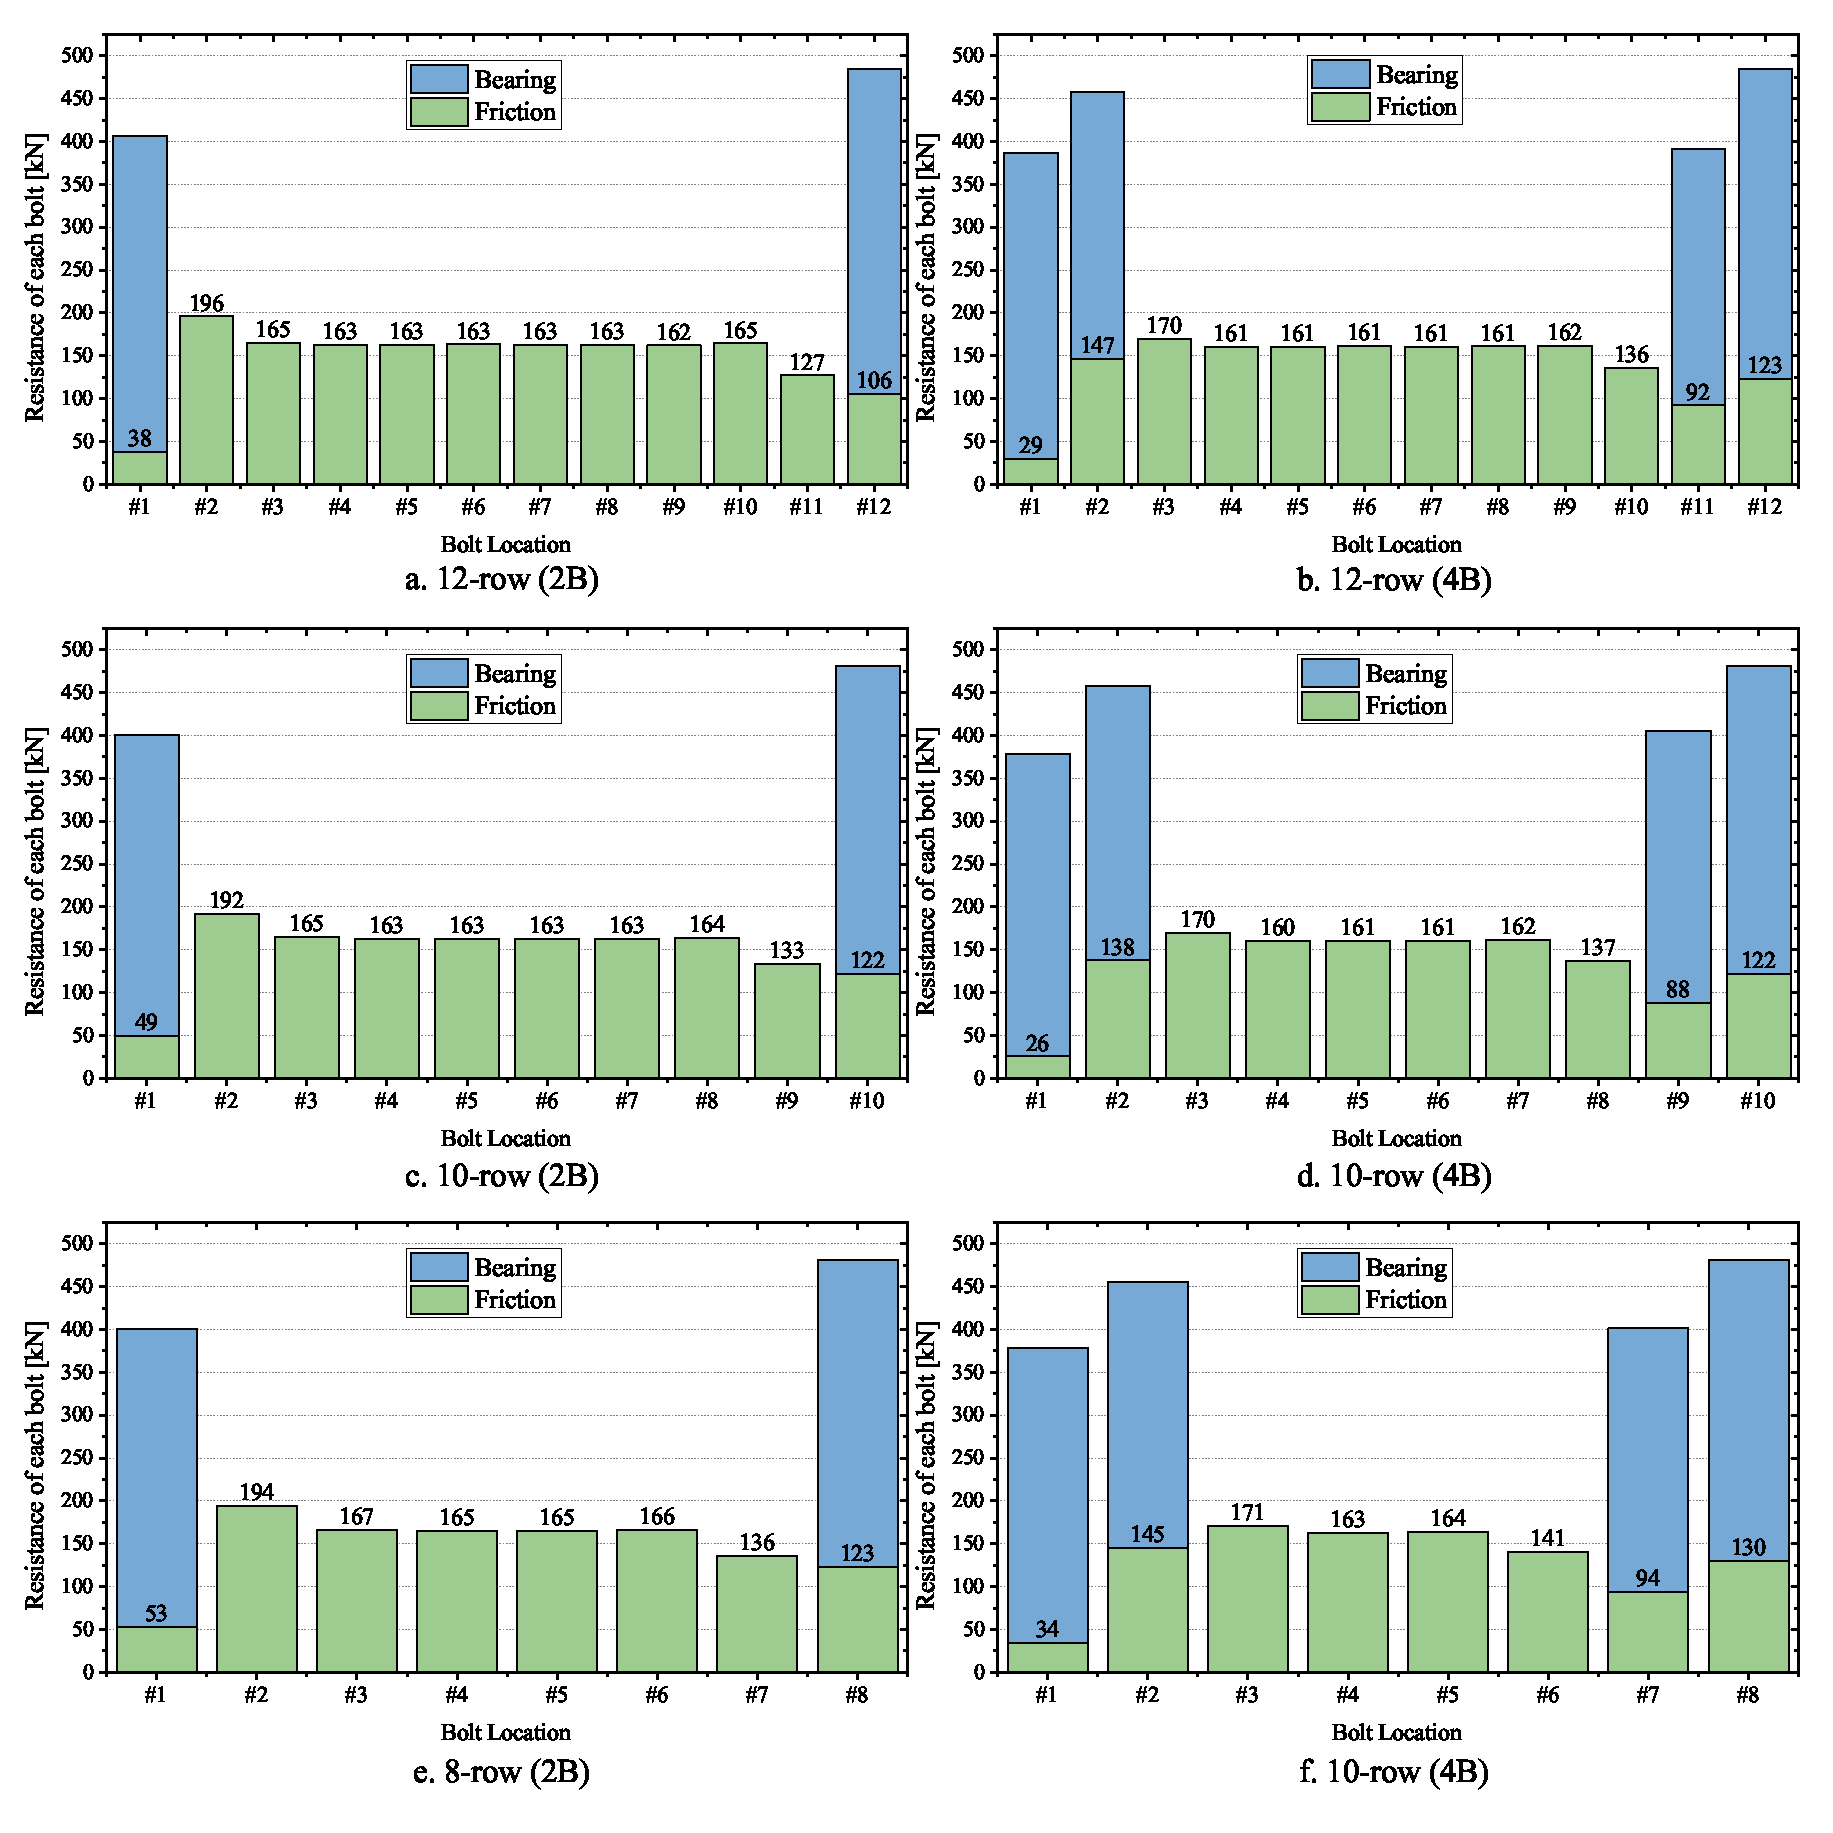
\includegraphics[width=\linewidth]{imgs/ch7/LS-all.eps}
    \caption{Load sharing of each bolt (stacked bar = friction load $P_{s1}$ + bearing load $P_{b1}$)}
    \label{fig-ls-all}
\end{figure*}

Figure \ref{fig-ls-all} shows the distribution of friction and bearing resistance on individual bolts when the load reaches bolt shear yielding in the bolt shank (SLS) for different bolt arrangements. The green bars represent the resistance transferred load through friction for each bolt, whereas the blue bars represent the resistance transferred load through the bearing. For long bolted connections, owing to the uneven load distribution, the bolts located in the middle of the connection cannot reach their actual design slip strength when the joint reaches the allowable slip value \cite{KAMEI2000,peng2013}. Therefore, the JSHB \cite{douji2017} proposes a reduction factor for long bolted connections. However, for hybrid joints, the bolts for friction connections arranged in the middle have a uniform load sharing and all bear the load of their design slip resistance ($F_s = \mu m N=0.4\times 2 \times 205 = 164 kN$). Additionally, for the fit bolts, owing to their bearing load transfer mechanism, the friction forces experienced varying degrees of reduction. The \# 1 bolt at the front experienced the most severe reduction in friction resistance, which is explained in detail in Section \ref{sec-decoff}. Meanwhile, for the bearing resistance borne by the fit bolts, when the number of fit bolts was four (i.e., two at each end), uneven load sharing occurred. Although it appears that the \# 2 bolt bears more load ($P_b + P_s$), the \# 1 bolt at the front has almost no friction force remaining owing to the deformation; thus, it relies almost entirely on the bearing to transfer the load. Consequently, the transferred bearing resistance was the highest of all the fit bolts, causing the bolt shank shear yield to occur first in bolt \# 1. In addition, the bearing resistance $P_{b}$ cannot reach the design bearing strength $F_b$ because of the uneven bearing load distribution.


\subsection{Reduction of friction force}
\label{sec-decoff}

\begin{figure*}
    \centering
    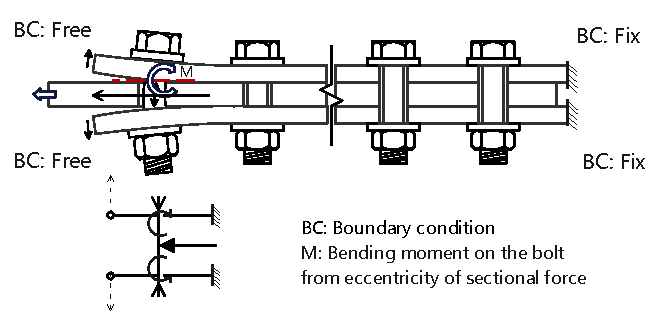
\includegraphics[width=0.7\linewidth]{imgs/ch7/OP-def.pdf}
    \caption{Schematic of out-plane deformation for splice plates}
    \label{fig-OP-def}
\end{figure*}

The cross-sectional force on the main plate was divided into the cross-sectional forces of the main plate and splice plates via shear transmission on the bolt, as shown in Figure \ref{fig-OP-def}. Assuming that the point of action of each cross-sectional force is at the centre of the plate, an additional bending moment is generated in the bolt owing to the eccentricity of the cross-sectional forces. The boundary condition at the end of the connection plate is free, so it tends to deform outwards towards the main plate faying surface when subjected to additional bending moments, resulting in the separation of the connection plate from the main plate.

\begin{figure}[htbp]
    \centering
    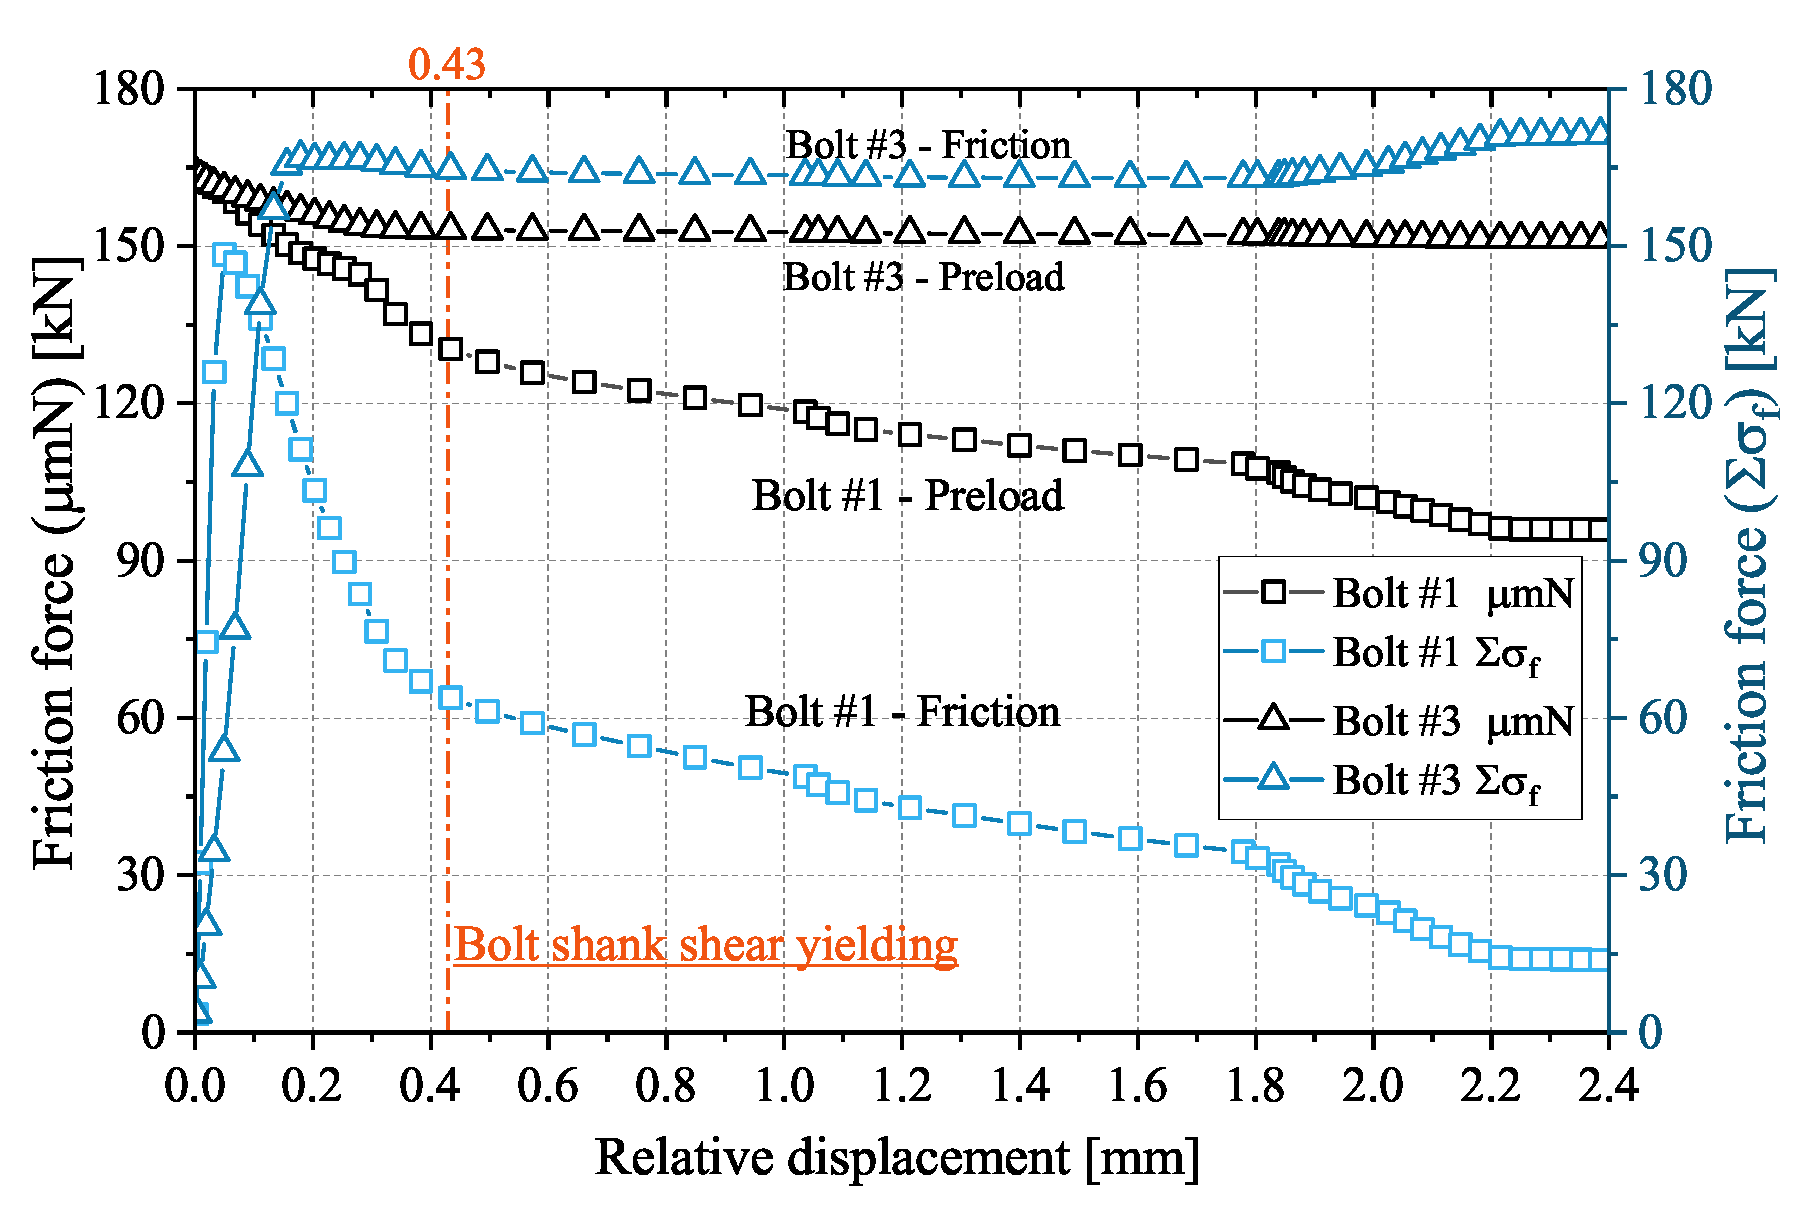
\includegraphics[width=0.7\linewidth]{imgs/ch7/RD2NF.eps}
    \caption{Relationship between \# 1, \# 3 bolt's friction force based on the integration of shear stress $\sigma_f$ and the friction force based on preload ($\mu m N = 0.4 \times 2 \times N$) to relative displacement (OA4B case).}
    \label{fig-RD2NF}
\end{figure}

Figure \ref{fig-RD2NF} shows the Relationship between \# 1, \# 3 bolt's friction force based on the integration of shear stress $\sigma_f$ ($\sum \sigma_f A_f$) and the friction force based on preload ($\mu m N = 0.4 \times 2 \times N$) to relative displacement (OA4B case). Where the bolt preload $N$ is obtained through the built-in bolt load option in Abaqus. It can be observed that due to the shear deformation of bolt \# 1, it experiences a loss of preload. However, the friction force obtained based on the bolt preload is higher than that calculated from the contact surface. In addition to the loss of preload, the reduction in friction force is also attributed to the separation and the resulting gap between the end contact surfaces (as explained in the next paragraph). On the other hand, the HSB-FC located at position \# 3 does not undergo shear bending, so its preload and the resulting friction force do not change significantly.


\begin{figure*}
    \centering
    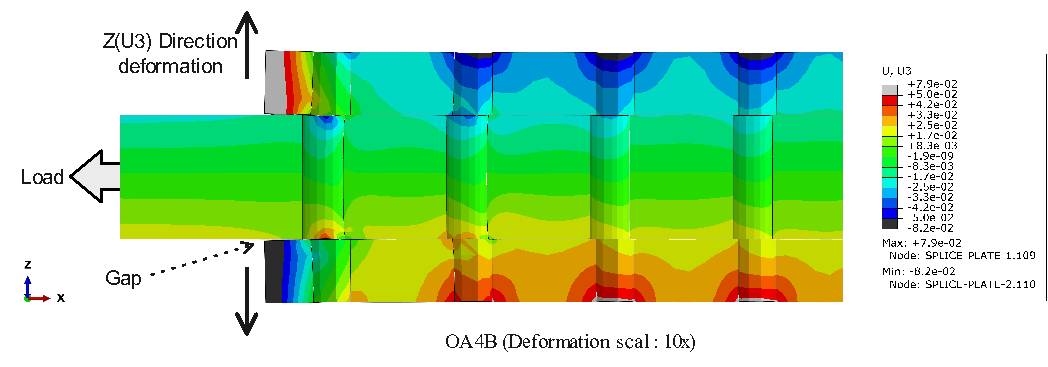
\includegraphics[width=0.8\linewidth]{imgs/ch7/OP-def-ana.pdf}
    \caption{Counter of the deformation at the U3 (z) direction when bolt shank shear yielding occurs (Relative displacement E-10mm = 0.43 mm). (Deformation scale: 10X).}
    \label{fig-OP-def-ana}
\end{figure*}

\begin{figure*}
    \centering
    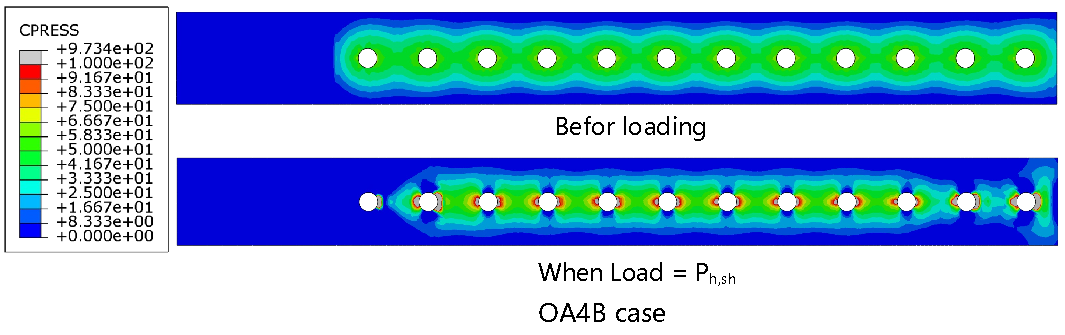
\includegraphics[width=0.8\linewidth]{imgs/ch7/OA4B-cpress.pdf}
    \caption{C-Press contour view of the main plate's faying surface}
    \label{fig-cpress}
\end{figure*}

Figure \ref{fig-OP-def-ana} shows the deformation contour plot of the joint in the U3 (z) direction, where it is evident that the splice plate underwent deformation owing to the additional bending moment generated. When the connection is at bolt shank shear yielding (SLS), the relative displacement at E-10mm is 0.43 mm, while the maximum out-of-plane deformation at U3 (in the z-direction) at the end is 0.07 mm.

On the compressed side of the bolt, where the bolt generates an additional bending moment owing to bolt deformation, a higher contact pressure is generated at the compressed side, as shown in Figure \ref{fig-cpress}. However, there was an overall decreasing trend in the total contact pressure on the faying surface.



\subsection{Reduction of bearing force} \label{sec-rduc-bea}

\begin{figure*}
    \centering
    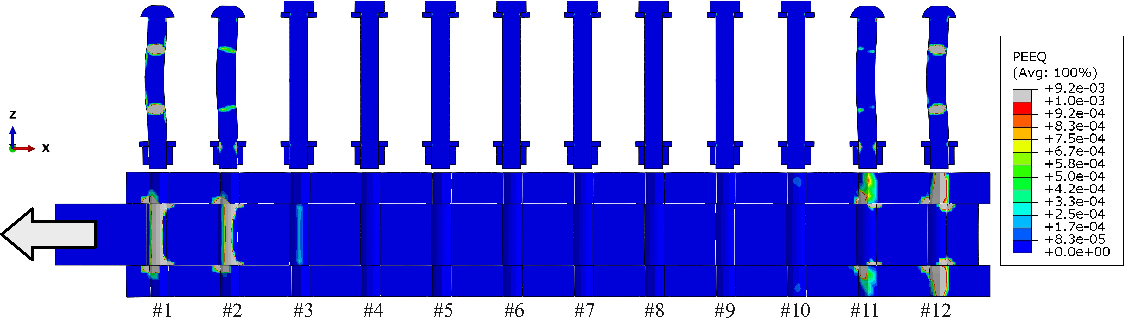
\includegraphics[width=0.9\linewidth]{imgs/ch7/beadist.pdf}
    \caption{Counter of PEEQ when bolt shank shear yielding occurs (OA4B case)}
    \label{fig-bsh}
\end{figure*}


Figure \ref{fig-bsh} shows the PEEQ contours for the bolt and steel plate when bolt \# 1 experiences bolt shank shear yielding $P_{h,sh}$ in the OA4B case. When two bolts were arranged at each end, the bearing forces on the bolts were unevenly distributed. When bolt \# 1 experienced yielding at the shear plane, the shear plane of bolt \# 2 entered plastic elongation. Owing to their symmetry, bolts \# 11 and \# 12 exhibited almost the same behaviour.

\subsection{Reduction factor of bolt shank shear resistance for hybrid connection}



\begin{figure}[htbp]
    \centering
    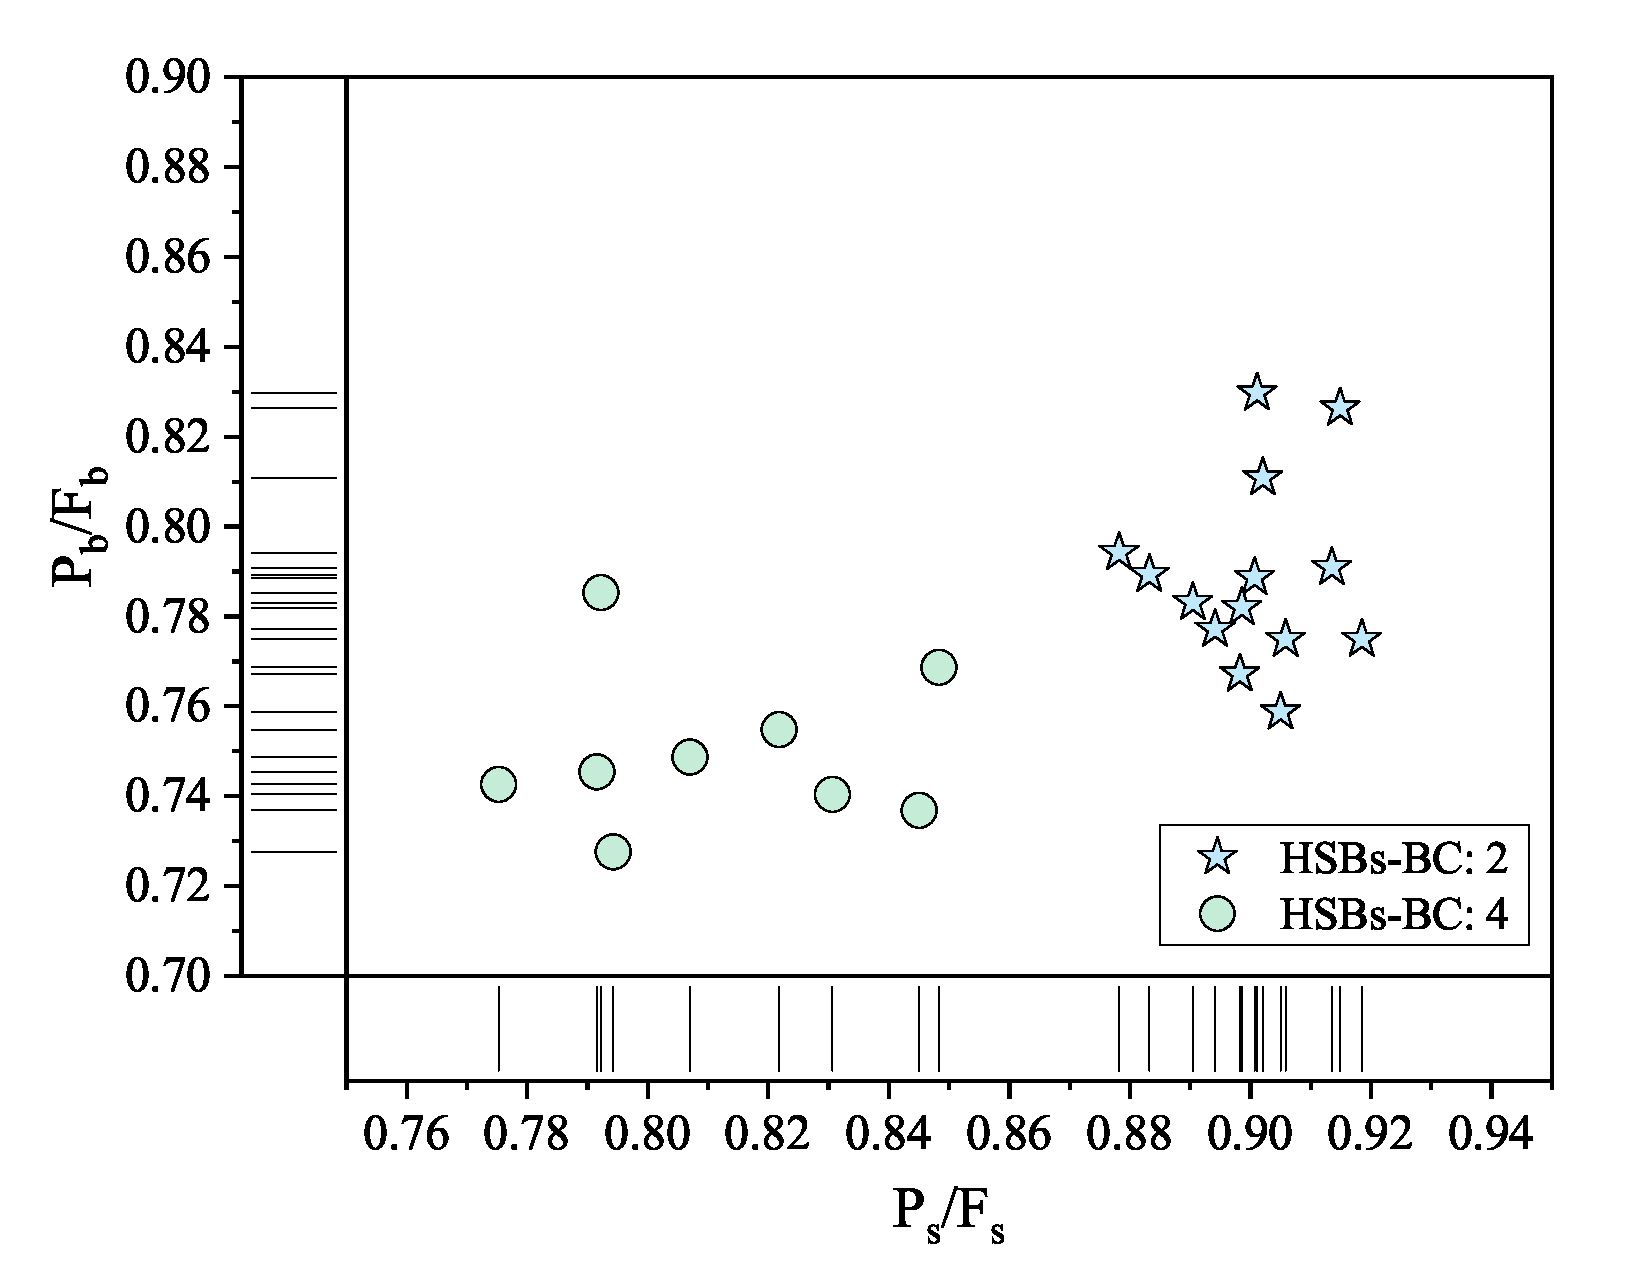
\includegraphics[width=0.65\linewidth]{imgs/ch7/RF-pspb.eps}
    \caption{Distribution of the reduction rates of bearing / friction resistance}
    \label{fig-dist-RF}
\end{figure}

Owing to the different load transfer mechanisms of friction and bearing, this study explored the reduction in friction and bearing forces separately to evaluate the bolt shank shear yielding strength of the hybrid joint more accurately. Formulas for the reduction factors based on the friction and bearing forces were proposed, as shown in Eq. \ref{eq-pvh-2}. 

Figure \ref{fig-dist-RF} shows the reduction rates of the friction force ($P_s/F_s$) and bearing force ($P_b/F_b$). The distribution range of the friction force reduction rate ($P_s/F_s$) is larger than that of the bearing ($P_b/F_b$). Regarding the reduction rates of the friction force, the cases with four fit bolts (green circles in the Figure \ref{fig-dist-RF}) were widely scattered, whereas the cases with two fit bolts (blue pentagons) were concentrated within a smaller range ($0.9 \pm 0.02$). This is because for the cases with four fit bolts, owing to the uneven distribution of the bearing loads, the friction forces were also affected to varying degrees. When four fit bolts were used, the variation in the friction force reduction rate was slightly larger. For the bearing force, the variation in the reduction rate was relatively small; the reduction rates of the cases with four fit bolts were concentrated at approximately 0.74, whereas those of the cases with two bolts were concentrated at approximately 0.79.

\begin{table*}[htbp]
    \small
    \centering
    \caption{Reduction factor of the bearing and friction forces}
    \begin{tabularx}{\textwidth}{@{}lcccccccccc@{}}
    \toprule
     & $n_{cases}$ & Mean & SD  & CV [\%] & SE & Lo- 99\% CI & Up- 99\% CI & Min & Median & Max \\ \midrule
     \multicolumn{11}{c}{For $P_b/F_b$}\\
     Fit bolts: 2 & 14 & 0.79 & 0.021 & 2.6 & 0.005 & 0.77 & 0.80 & 0.76 & 0.79 & 0.83 \\
     Fit bolts: 4 & 9  & 0.75 & 0.017 & 2.3 & 0.006 & 0.73 & 0.76 & 0.73 & 0.75 & 0.79 \\ 
     Total        & 23 & 0.77 & 0.027 & 3.5 & 0.006 & 0.76 & 0.79 & 0.73 & 0.78 & 0.83 \\\midrule
     \multicolumn{11}{c}{For $P_s/F_s$}\\
     Fit bolts: 2 & 14 & 0.90 & 0.011 & 1.3 & 0.003 & 0.89 & 0.91 & 0.88 & 0.90 & 0.92 \\
     Fit bolts: 4 & 9  & 0.81 & 0.027 & 3.4 & 0.009 & 0.79 & 0.83 & 0.78 & 0.81 & 0.85 \\
    Total         & 23 &0.86 & 0.047 & 5.5 &0.01 &0.84 &0.89 &0.78 &0.89 &0.92 \\
     \bottomrule 
     \multicolumn{11}{r}{SD:Standard Deviation; CV: Coefficient of Variation; SE: Standard Error; CI: Confidence Interval} \\ 
    \end{tabularx}
    \label{tab-rdfactor}
\end{table*}

Table \ref{tab-rdfactor} summarises the load reduction rates of the bearing and friction forces for cases with two and four fit bolts, providing key statistical metrics. For the bearing force reduction rate, the coefficient of variation (CV) is consistently low (around 2-3\%) regardless of the number of fit bolts. In contrast, the friction force reduction rate shows more variability, with a CV of 1.2\% for two fit bolts and 3.3\% for four fit bolts. This suggests that the bolt arrangement has a more significant impact on the dispersion of the friction force reduction rate compared to the bearing force reduction rate.

Given these observations, this study adopts separate reduction factors for cases with two and four fit bolts, using the lower 99\% CI values for both bearing and friction forces. The reduction factors $\alpha_b$ for the bearing force and $\alpha_s$ for the friction force are defined as shown in Eq. \ref{eq-as}.

\begin{equation}
    \begin{aligned}
        F_{h,sh,cor} = \alpha_s F_s+\alpha_{b} F_b
    \end{aligned}
    \label{eq-pvh-2}
\end{equation}

Where,

\begin{tabularx}{0.95\linewidth}{ l X }
$\alpha_s$ & the reduction factor for the slip resistance;\\ 
$\alpha_b$ & the reduction factor for the bearing resistance of fit bolts.\\
\end{tabularx}

\begin{equation}
\alpha_s =
\begin{cases} 
0.89  \\ 
0.79
\end{cases} \space ; 
\alpha_b = \begin{cases}
0.77 & \text { if } n_b = 2\\
0.73 & \text { if } n_b = 4
\end{cases}
\label{eq-as}
\end{equation}


\begin{figure*}
    \centering
    % \begin{subfigure}[b]{0.32\textwidth}
    %     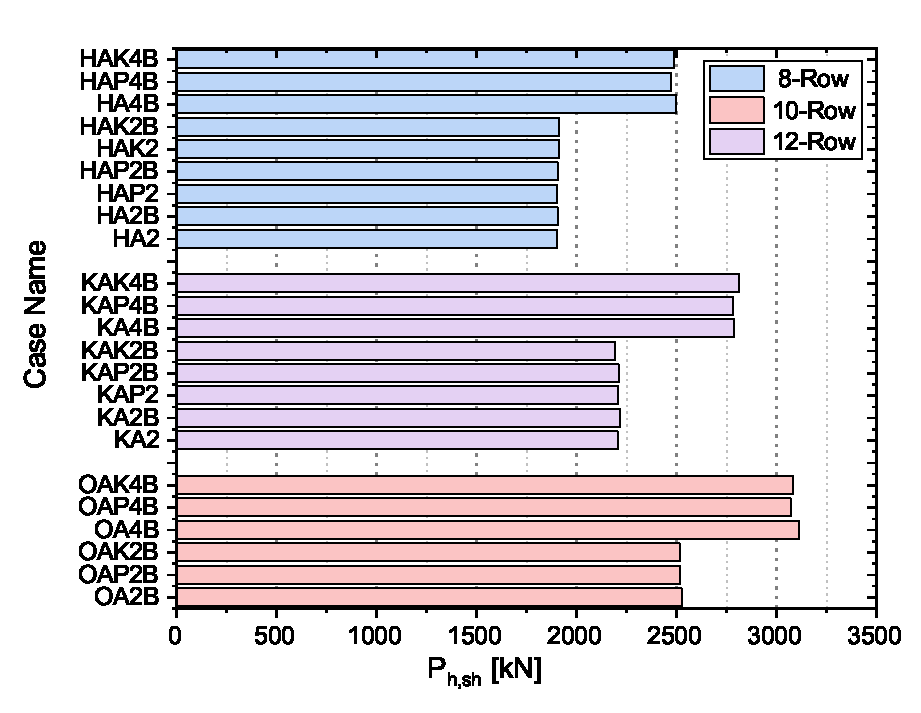
\includegraphics[width=\linewidth]{imgs/ch7/RF-capa-bar.eps}
    %     \caption{Analysis value of bearing force $P_{h,sh}$}
    %     \label{fig-pb-bar}
    % \end{subfigure}
    % \hfill
    \begin{subfigure}[b]{0.45\textwidth}
        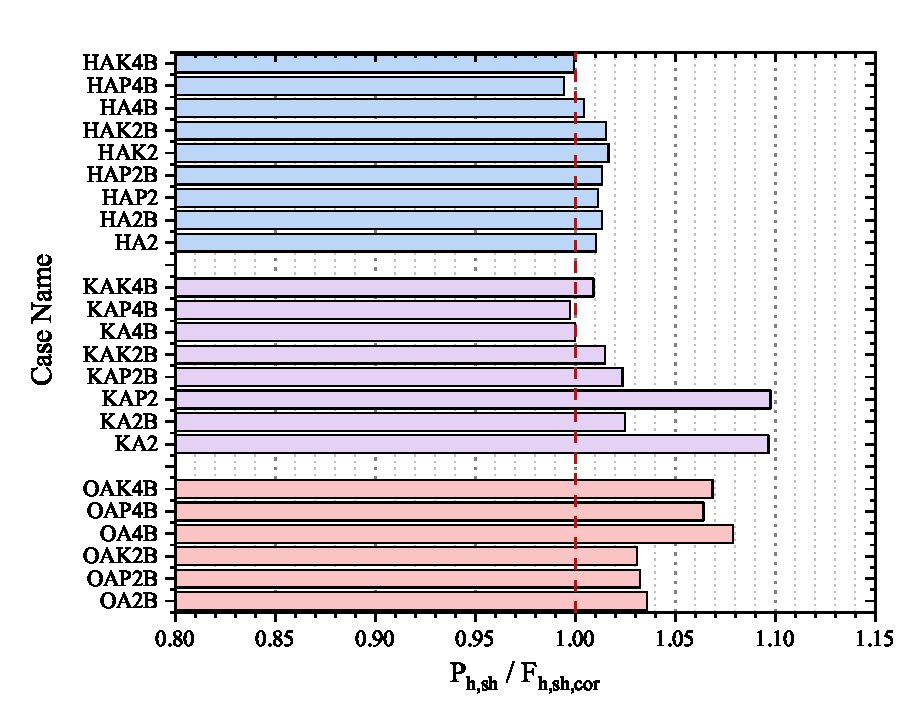
\includegraphics[width=\linewidth]{imgs/ch7/RF-total-cor.eps}
        \caption{Simple accumulate ($F_{h,sh}=F_s+F_b$)}
        \label{fig-fhv}
    \end{subfigure}
    \hfill
    % \begin{subfigure}[b]{0.48\textwidth}
    %     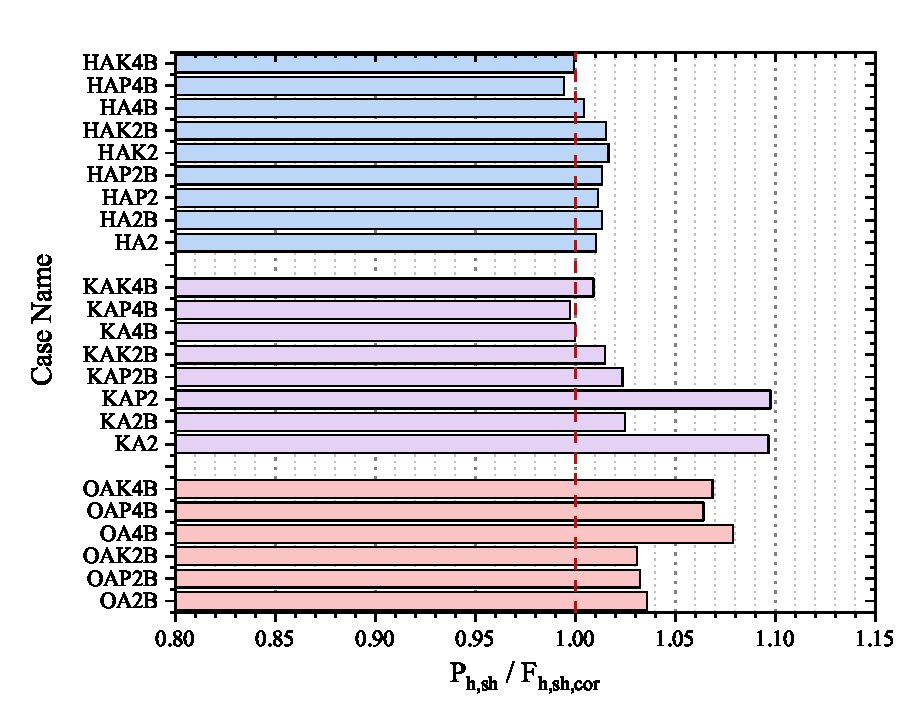
\includegraphics[width=\linewidth]{imgs/ch7/RF-total-cor.eps}
    %     \caption{After correction - 1 , (Equation \ref{eq-fbh2-1}, Equation \ref{eq-fbh4-1})}
    %     \label{fig-fhv-cor1}
    % \end{subfigure}
    % \centering
    \begin{subfigure}[b]{0.45\textwidth}
        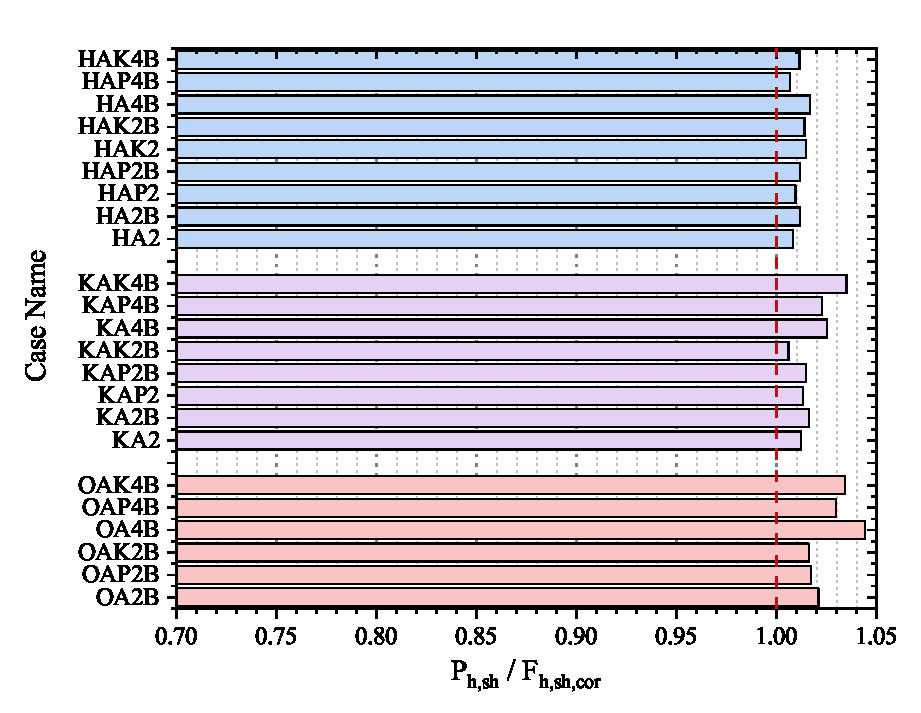
\includegraphics[width=\linewidth]{imgs/ch7/RF-total-cor-2.eps}
        \caption{With correction factor, (Equation \ref{eq-pvh-2})}
        \label{fig-fhv-cor2}
    \end{subfigure}
    \caption{Relationship between the analysis value $P_{h,sh}$ and the calculated hybrid bolt shank shear yield resistance ($F_{h,sh}, F_{h,sh,cor}$) of each case}
    \label{fig-fhv-total}
\end{figure*}

 Figure \ref{fig-fhv-total} shows the ratio between the analytical results ($P_{h,sh}$) and the calculated values ($F_{h,sh}$, $F_{h,sh,cor}$) for each case. The dashed red line represents a ratio of 1 (i.e., the calculated result matches the analytical result). 

In figure \ref{fig-fhv}, for the simple accumulate calculation formula $F_{h,sh}$, the analytical result $P_{h,sh}$ deviates significantly from the calculated value $F_{h,sh}$. And it can be observed that the simplified calculation overestimated the bearing capacity of fit bolts, resulting in greater discrepancies in the calculation results of the -4B case compared to the -2B case.


Figure \ref{fig-fhv-cor2} shows the calculated values obtained by separately reducing the friction and bearing forces (Eq. \ref{eq-pvh-2}). The analytical results and calculated values match well, with the analytical results only slightly exceeding the calculated values, which can be considered a safe design. Even in the KA2 and KAP2 cases, where $\beta_h$ ($F_h/F_y$) is close to one, the results are satisfactory, suggesting that the calculation formula is relatively accurate.

Additionally, in Figure \ref{fig-fhv-cor2}, for the cases with four fit bolts, the results obtained for eight, 10, and 12 rows differed. The fewer the rows (e.g., blue bar, HA case), the closer the result is to the calculated value, and the more the rows, the higher the result compared to the calculated value. This is because the greater the number of rows, the less impact the loss of friction force due to the bearing deformation of the fit bolts has on the overall reduction rate of the friction force. As shown in Eq. \ref{eq-intr-as}, the reduction factor for the friction force is mainly divided into two parts. The first is fit bolt \#1 at the end, which lost almost all the friction force owing to deformation; therefore, the friction force of \#1 was not considered, as represented by $n_b-1$. The other part comprises the remaining fit bolts, whose friction force also experienced an uneven load distribution owing to the uneven bearing force, represented by $\alpha_{s,b}$, which is described in detail in Section \ref{sec-rduc-bea}. This can explain why, if the number of rows increases, $n_s$ will also increase, and the reduction brought about by $n_b-1$ and $\alpha_{s,b}$ will be lower, resulting in $P_{h,v}/F_{h,v,cor}$ for 12 rows (orange bar) being higher relative to eight rows (blue). The effect of the number of bolt rows (connection length) on the frictional force reduction factor is discussed in the next section.

\begin{equation}
    \alpha_s F_s \approx ((n_f+ (n_b-1)\alpha_{s,b}) F_{s1} ) 
    \label{eq-intr-as}
\end{equation}


\subsection{Reduction of joint length}

\begin{figure}[htbp]
    \centering
    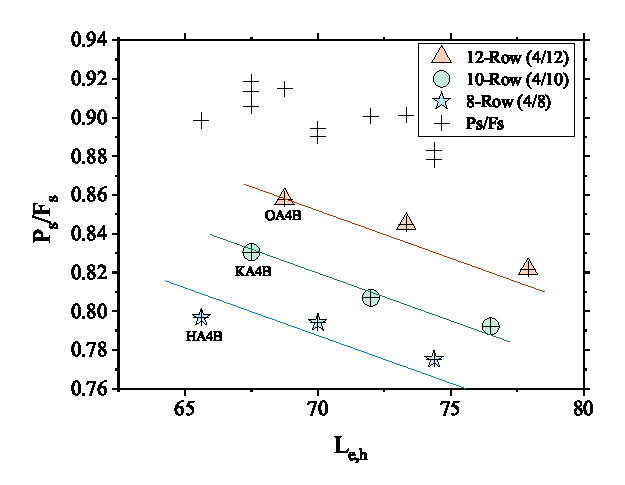
\includegraphics[width=0.65\linewidth]{imgs/ch7/as-leh.eps}
    \caption{ $\alpha_s ((P_b-P_{b,\#1})/((n_b)F_{shy1})$ and effective joint length $L_{e,h}$}
    \label{fig-rdc-leh}
\end{figure}

Figure \ref{fig-rdc-leh} shows the relationship between the friction force reduction rate and the effective length of the hybrid joint, $L_{e,h}$ (non-dimensionalized by the number of bolt rows, $L_{e,h} = L_J / n_b$). The coloured plots represent cases with four fit bolts, where the orange triangles represent 12 rows of bolts, green circles represent 10 rows of bolts, and blue triangles represent eight rows of bolts. For the cases with four fit bolts, as the effective joint length increases, the friction force reduction rate decreases. For the cases with two fit bolts (represented by the + symbol), no obvious relationship between the friction force reduction rate and joint effective length was found. 




% \section{SLS for hybrid connection}

% According to the numerical analysis in the previous section and the comparison with the experimental results, although JSHB follows the formula $1.7f_y$ for the design of the \ac{ASD} methods, it can be found that this formula is too high for evaluating the limit state of the use of the bearing connection, especially for the hybrid joint, the bearing connection always has to share more force than the general bolts, so for the design of bearing resistance for the hybrid connection, the present study concludes that It is more reliable to cancel the coefficient before yield strength, and the design formula for bearing yield resistance for one fastener $F_{by1}$ is as follows:

% \begin{equation}
%     F_{by1} = dtf_y
% \end{equation}

% In this study, it is considered that the bearing connection in the use of limit state in addition to the bearing yield will also appear fastener shear yield, fastener shear yield for one fastener $F_{vy1}$ can be calculated by the following formula to obtain.

% \begin{equation}
%     F_{vy1} = A_s f_{yb}/\sqrt{3}
% \end{equation}

% the slip resistance per fastener shall taken as:

% \begin{equation}
%     F_{s1} = m \mu N_0
% \end{equation}


% For the resistance of hybrid joints, this study suggests that the resistance of a hybrid joint can be obtained directly by adding the smaller of the bearing yield resistance and the shear yield resistance of the person and the slip resistance, however, this is only the ideal state, and the actual strength will be affected by the following two main aspects, 1. Slip resistance attenuation of Kinetic friction $\alpha_{kf}$, 2. reduction of bolt preload due to bolt was under shear yield $\alpha_{v}$, and 3. Friction/bearing load sharing mechanism $\beta_{ls}$. These two factors primarily determine the magnitude of slip strength and bearing resistance when added together. Preliminarily, this can be calculated by the following formula:

% For bolt shear yield resistance:

% \begin{equation}
%     F_{hv} = (n_f + \alpha_{v}(n_b-1)) F_s + \beta_{ls} n_b F_{vy})
% \end{equation}

% For bearing yield resistance:

% \begin{equation}
%     F_{hb} = n F_s + \beta_{ls} n_b F_{by}
% \end{equation}

% Where, $\alpha_{kf}$ is attenuation factor for kinetic friction, $\alpha_v$ is Correction factor for loss of preload due to shear failure, $\beta_{ls}$ is the correction factor for load sharing. $n$ is the number of the fastener, $n_f$ is the number of the fastener for friction type connections, $n_b$ is the number of the fastener for bearing type connections.

% \subsection{Fastener shear yield}

% In the bearing type connection, for the serviceability limit state, can be divided into two kinds, one is the fastener shear yield, the other is the bearing yield of the main plate, although the two kinds are one of the bearing limit state, in order to facilitate the calculation as well as to facilitate the differentiation, here will be the two kinds of limit state are discussed separately, and each of them has a different mechanical behavior.

% Table \ref{tabfe-shfst} lists the geometric information for this resolved case as well as the material and contact properties used. Table \ref{tabjr-sfst} lists the calculated resistance of the hybrid joints.

% \begin{table}[htbp]
% \centering
% \caption{Various property for FE analysis}\label{tabfe-shfst}
% \begin{tabular}{@{}cccccccccc@{}}
% \toprule
%  &
%   \begin{tabular}[c]{@{}c@{}}$w$\\ {[}mm{]}\end{tabular} &
%   \begin{tabular}[c]{@{}c@{}}$t$\\ {[}mm{]}\end{tabular} &
%   \begin{tabular}[c]{@{}c@{}}$d_0$\\ {[}mm{]}\end{tabular} &
%   \begin{tabular}[c]{@{}c@{}}Number of\\ bolt\end{tabular} &
%   \begin{tabular}[c]{@{}c@{}}Bolt for \\ bearing\end{tabular} &
%   $\mu$ &
%   \begin{tabular}[c]{@{}c@{}}$N_0$\\ {[}kN{]}\end{tabular} &
%   \begin{tabular}[c]{@{}c@{}}$f_y$\\ {[}Mpa{]}\end{tabular} &
%   \begin{tabular}[c]{@{}c@{}}$f_u$\\ {[}Mpa{]}\end{tabular} \\ \midrule
% shear-fst &
%   210 &
%   50 &
%   18 &
%   10 &
%   4 &
%   0.4 &
%   106 &
%   550 &
%   694 \\ \bottomrule
% \end{tabular}
% \end{table}


% \begin{table}[htbp]
% \centering
% \caption{Summary of joint resistance (unit: kN)}\label{tabjr-sfst}
% \begin{tabular}{@{}ccccccccc@{}}
% \toprule
%  &
%   \multicolumn{5}{c|}{SLS} &
%   \multicolumn{3}{c}{ULS} \\ \midrule
%  &
%   \begin{tabular}[c]{@{}c@{}}$F_s$\end{tabular} &
%   \begin{tabular}[c]{@{}c@{}}$F_{by}$\end{tabular} &
%   \begin{tabular}[c]{@{}c@{}}$F_{vy}$\end{tabular} &
%   \begin{tabular}[c]{@{}c@{}}$F_h$\end{tabular} &
%   \multicolumn{1}{c|}{\begin{tabular}[c]{@{}c@{}}$F_y$ \end{tabular}} &
%   \begin{tabular}[c]{@{}c@{}}$F_b$\end{tabular} &
%   \begin{tabular}[c]{@{}c@{}}$F_v$\end{tabular} &
%   \begin{tabular}[c]{@{}c@{}}$F_u$\end{tabular} \\ \cmidrule(l){2-9} 
% shear yield &
%   848 &
%   1760 &
%   835 &
%   1438 &
%   5280 &
  
%   5552 &
%   2320 &
%   6697 \\ \bottomrule
% \end{tabular}
% \end{table}


% Fig. \ref{fig-beafst} shows the The relationship between load and relative displacement when shear yield first case occurs. After the fastener shaft shear yielding occurred, two more slope changes occurred with a slight increase in slope due to the fact that on two separate occasions, the main plate bore wall contacted the bolt shaft used for the friction connection, and as the displacement continued to occur, the third time the slope changed to the contact between the connection plate and the fastener shaft. From this point on the connection forms a fully bearing type connection.

% \begin{figure}[htbp]
%     \centering
%     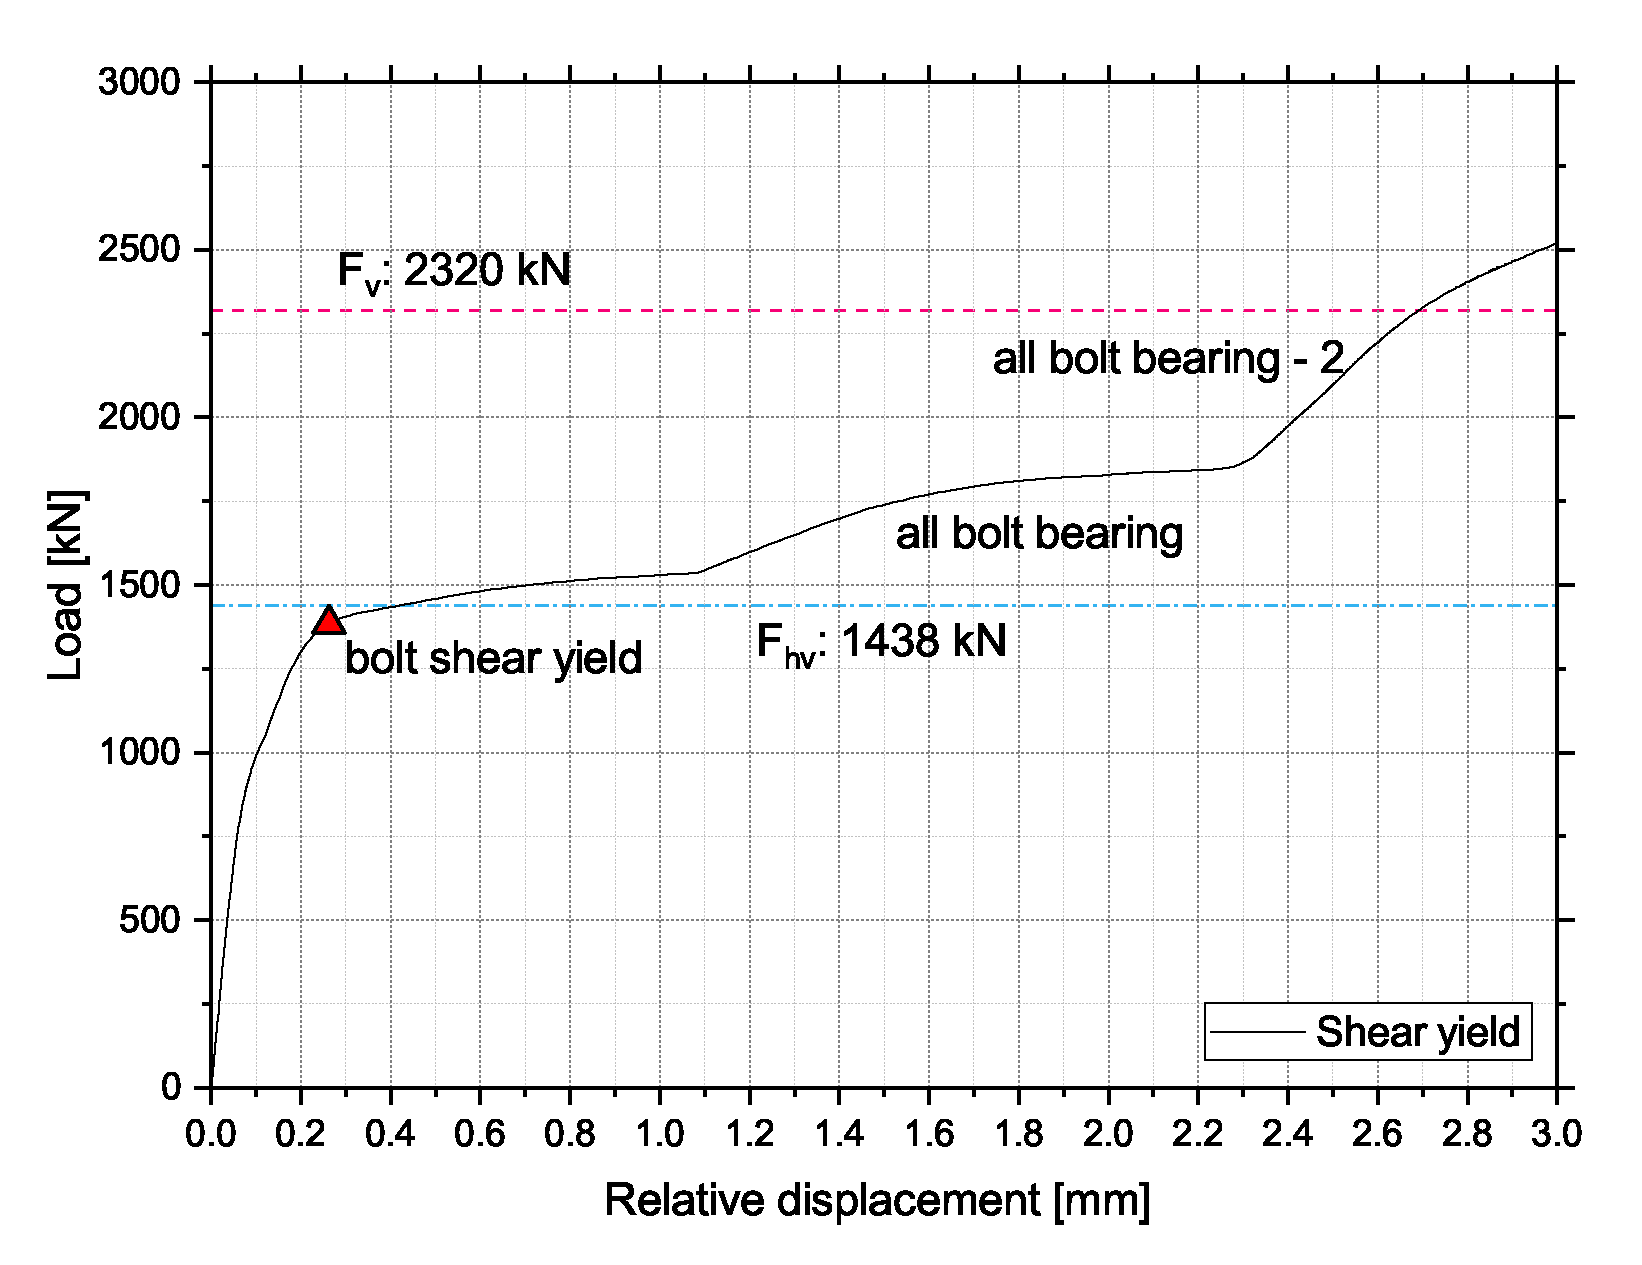
\includegraphics[width=0.8\textwidth]{imgs/ch7/M16b4-2.eps}
%     \caption{The relationship between load and relative displacement}
%     \label{fig-m16b4}
% \end{figure}

% Fig. \ref{fig-m16b4fvf} shows the Mises stress counter, from the figure can be found in the load of 1106kn, located in the end of the bolt in the shear surface occurred in the full cross-section yielding this and the curve occurred in the nonlinear (that is, the labeled point) position is approximately the same, which shows that the curve of the nonlinear behavior of the bolt by the shear yielding, and therefore can be considered to be the use of the bolt yielding the bolt of the limit state of hybrid joints

% \begin{figure}[htbp]
%     \centering
%     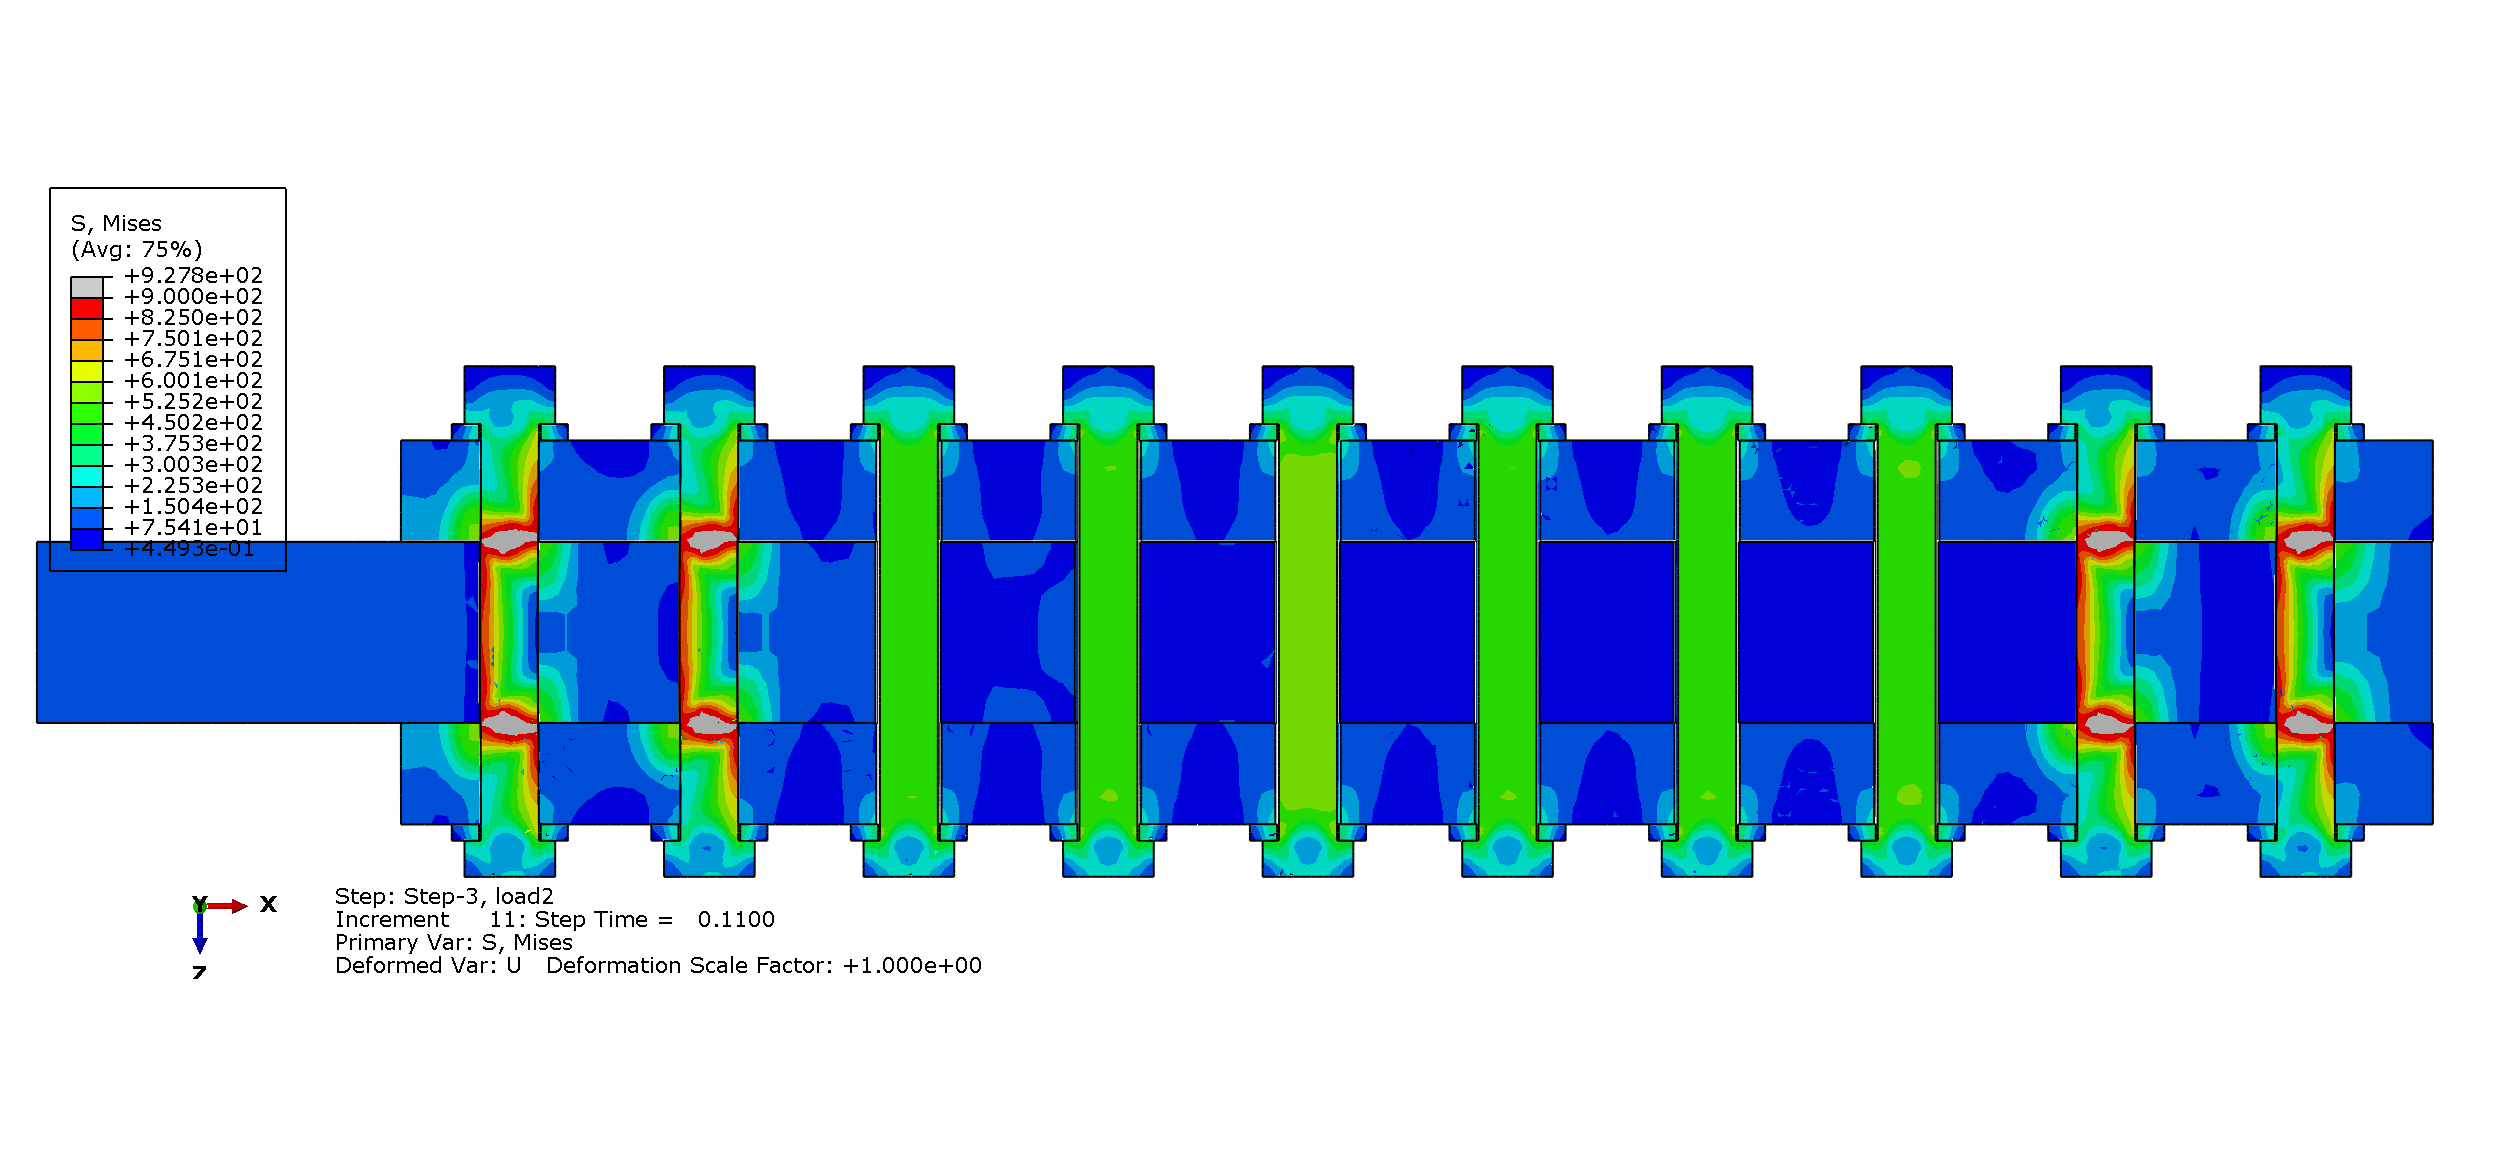
\includegraphics[width=0.8\textwidth]{imgs/ch7/M16b4-fvfst.png}
%     \caption{The fastener shear yield was occurred when load is equal to the 1384 kN}
%     \label{fig-m16b4fvf}
% \end{figure}


% \subsubsection{Reduction factor for bolt preload}

% %图1表示了当发生了螺栓截面剪切屈服时,螺栓轴力的降低情况。可以发现受剪切屈服的影响,端部用于承压连接的螺栓的轴力相对于中间的用于摩擦连接的螺栓的轴力的降低情况要大很多,端部4个螺栓的平均下降率低至0.76,也就是说用于承压连接的螺栓来说,当受到剪切屈服的影响时,轴力平均会下降至0.76,这个系数可以直接用于基于用于承压连接螺栓的折减系数。也可以对对于螺栓整体数量来进行折减,对于整体来说降低率为0.89(等效降低率).
% Fig. \ref{fig-b4ls} shows the reduction of the bolt preload when shear yielding of the bolt section occurs. It can be found that by the effect of shear yielding, the reduction of the preload of the bolts used for bearing connection at the end is much larger compared to the reduction of the preload of the bolts used for friction connection in the middle, and the average rate of reduction of the four bolts at the end is as low as 0.76, which means that for the bolts used for bearing connection, the preload decreases to an average of 0.76 when it is subjected to the effect of shear yielding, and this coefficient can be used directly for the reduction coefficient based on the bolts used for This coefficient can be directly used as a reduction factor for bolts used in connections under bearing pressure. This factor can be used directly for the reduction factor based on the number of bolts in the pressurized connection. It is also possible to reduce the number of bolts as a whole, with an overall reduction $\alpha_v$ of 0.89 (equivalent reduction rate).

% \begin{figure}[htbp]
%     \centering
%     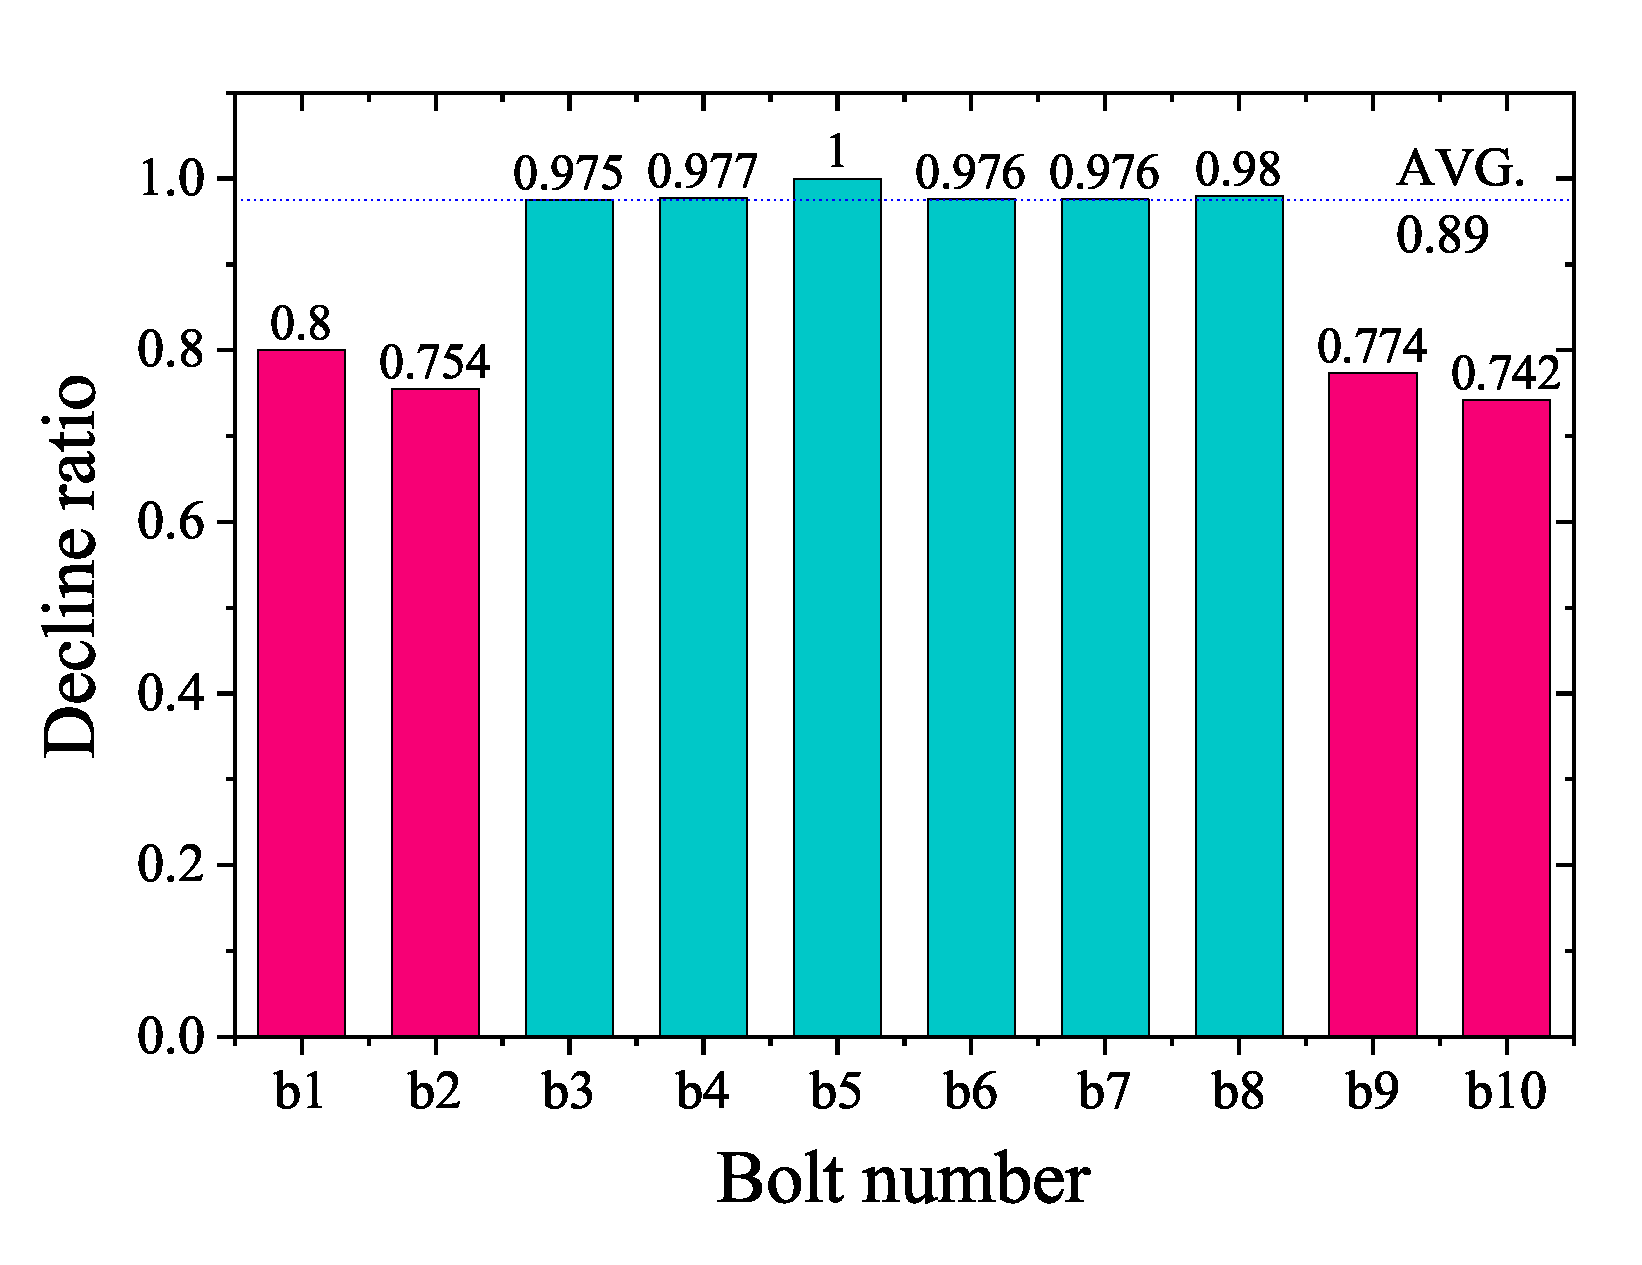
\includegraphics[width=0.7\textwidth]{imgs/ch7/b4-ls.eps}
%     \caption{Decline ratio of bolt preload when load is equal to the 1384 kN}
%     \label{fig-b4ls}
% \end{figure}

% \subsubsection{Reduction factor for front end fastener}

% Fig. \ref{fig-cstavfst} shows the CSTATUS counter when load is 1384 kN,Fig. \ref{fig-cstavfst} Deformation of z direction counter when load is 1384 kN.
% It can be observed that although the No.1 bolt at the end has residual axial force, due to the out-of-plane deformation of the connection plate (see Fig. \ref{fig-cstavfst}), most of the contact range of the \#1 bolt (b1) has completely changed from the original slipping state to the state of not in contact (see Fig. \ref{fig-cstavfst}), that is to say, in this area, the contact pressure is lost, resulting in friction failure, and therefore it is considered that the No.1 bolt at the end is not in contact. Friction and bearing pressure cannot work together when bearing pressure. When calculating the friction strength, n should be subtracted from 1.

% \begin{figure}[htbp]
%     \centering
%     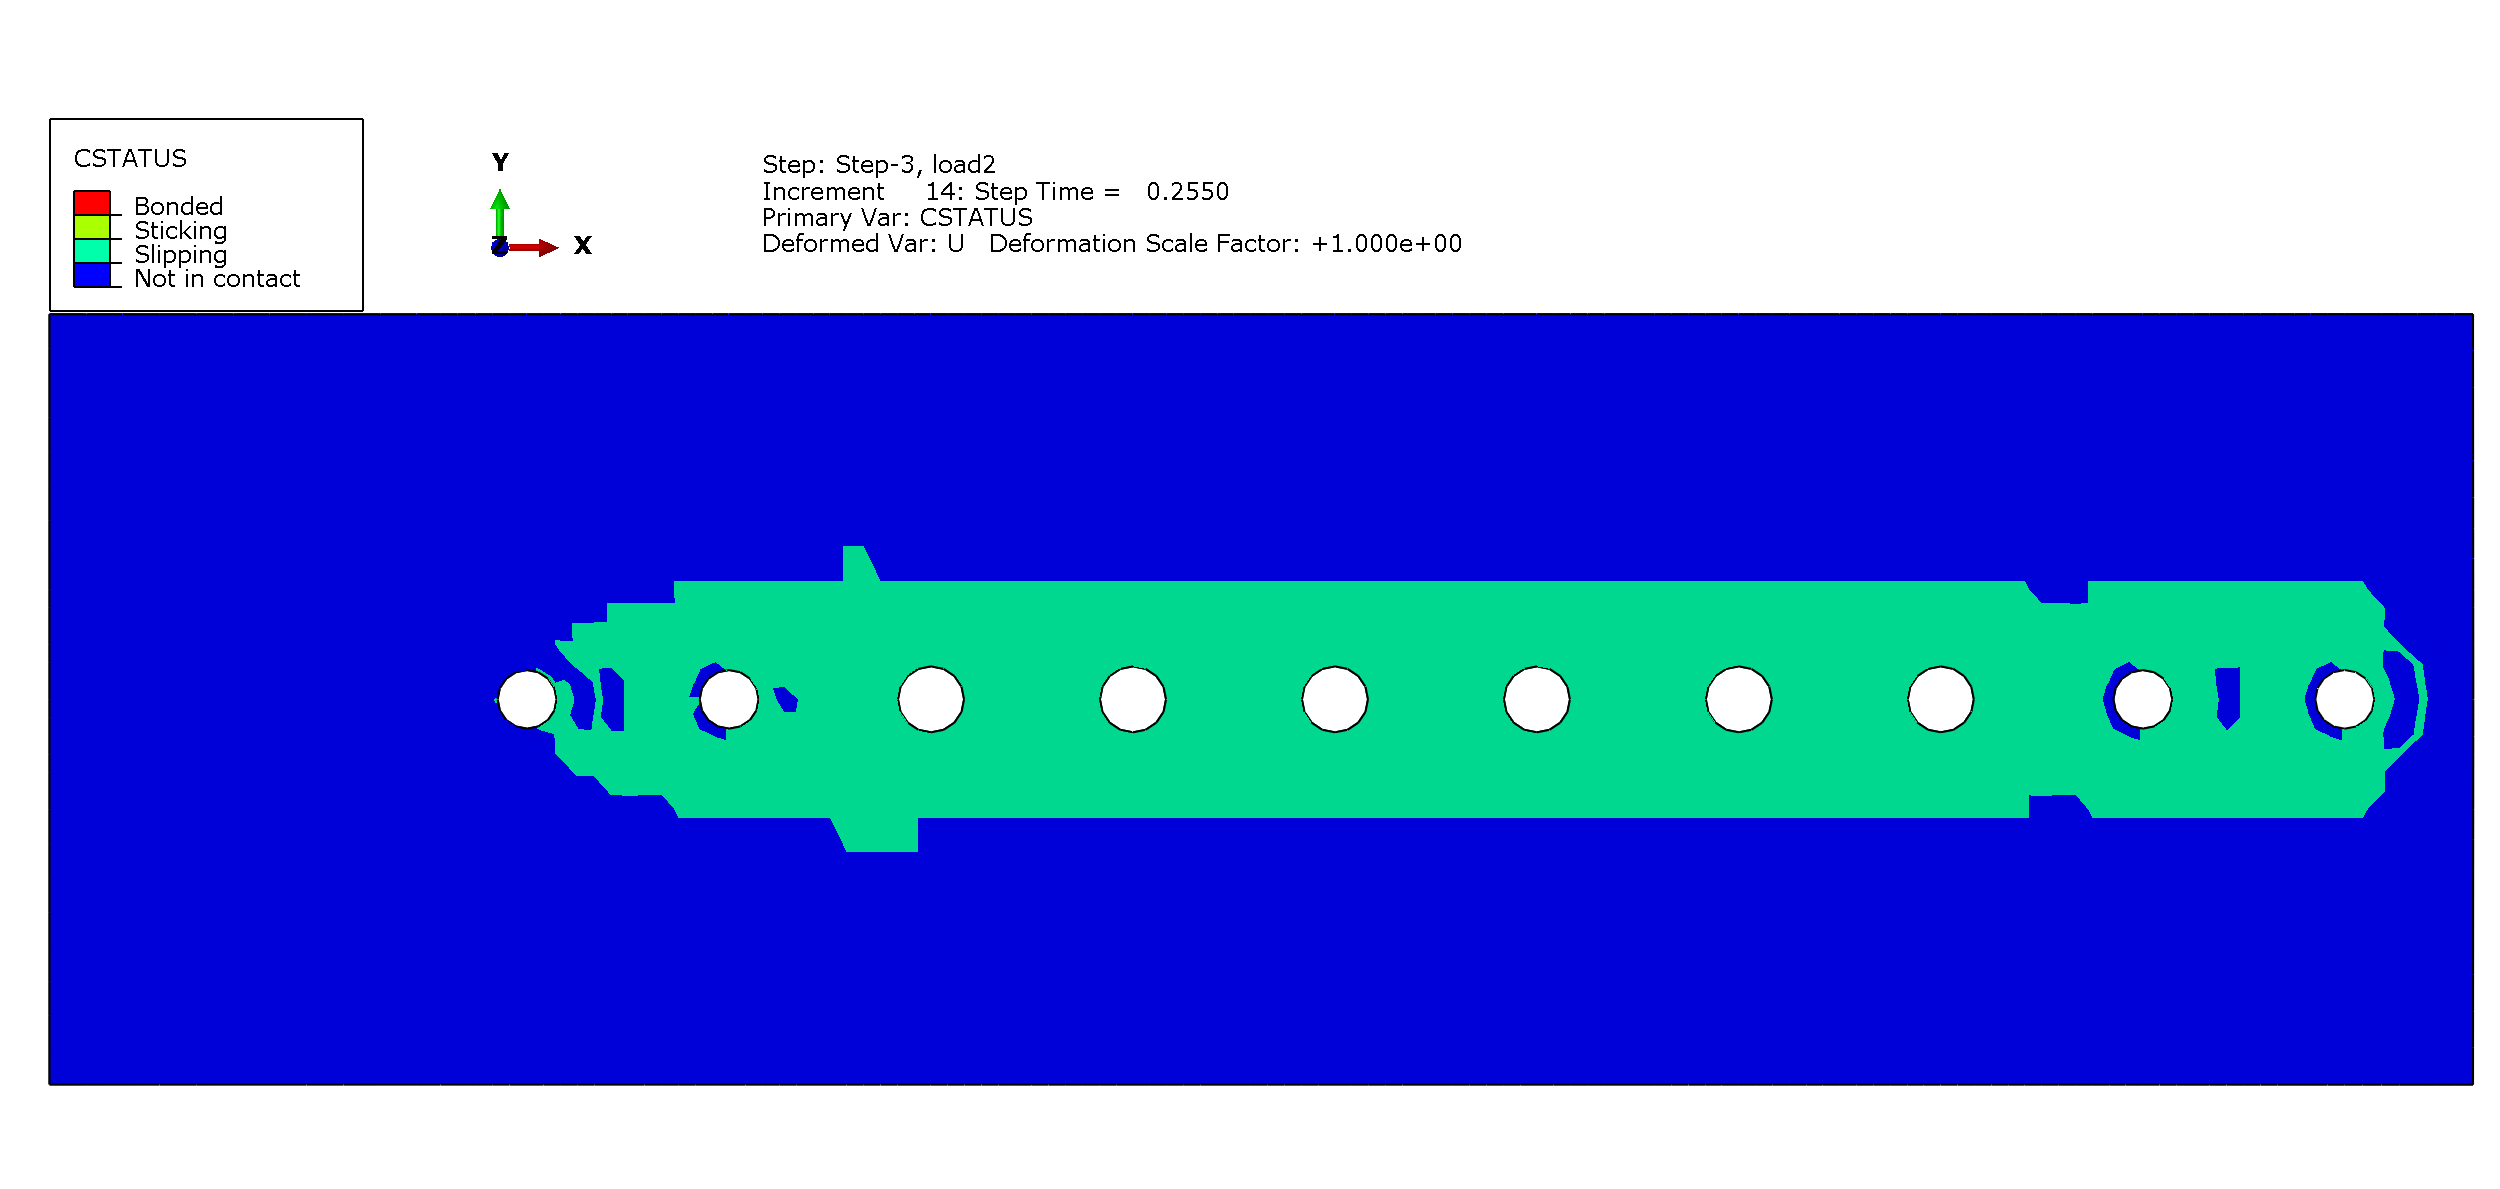
\includegraphics[width=0.8\textwidth]{imgs/ch7/cstatus-vfst.png}
%     \caption{CSTATUS counter when load is 1384 kN}
%     \label{fig-cstavfst}
% \end{figure}

% \begin{figure}[htbp]
%     \centering
%     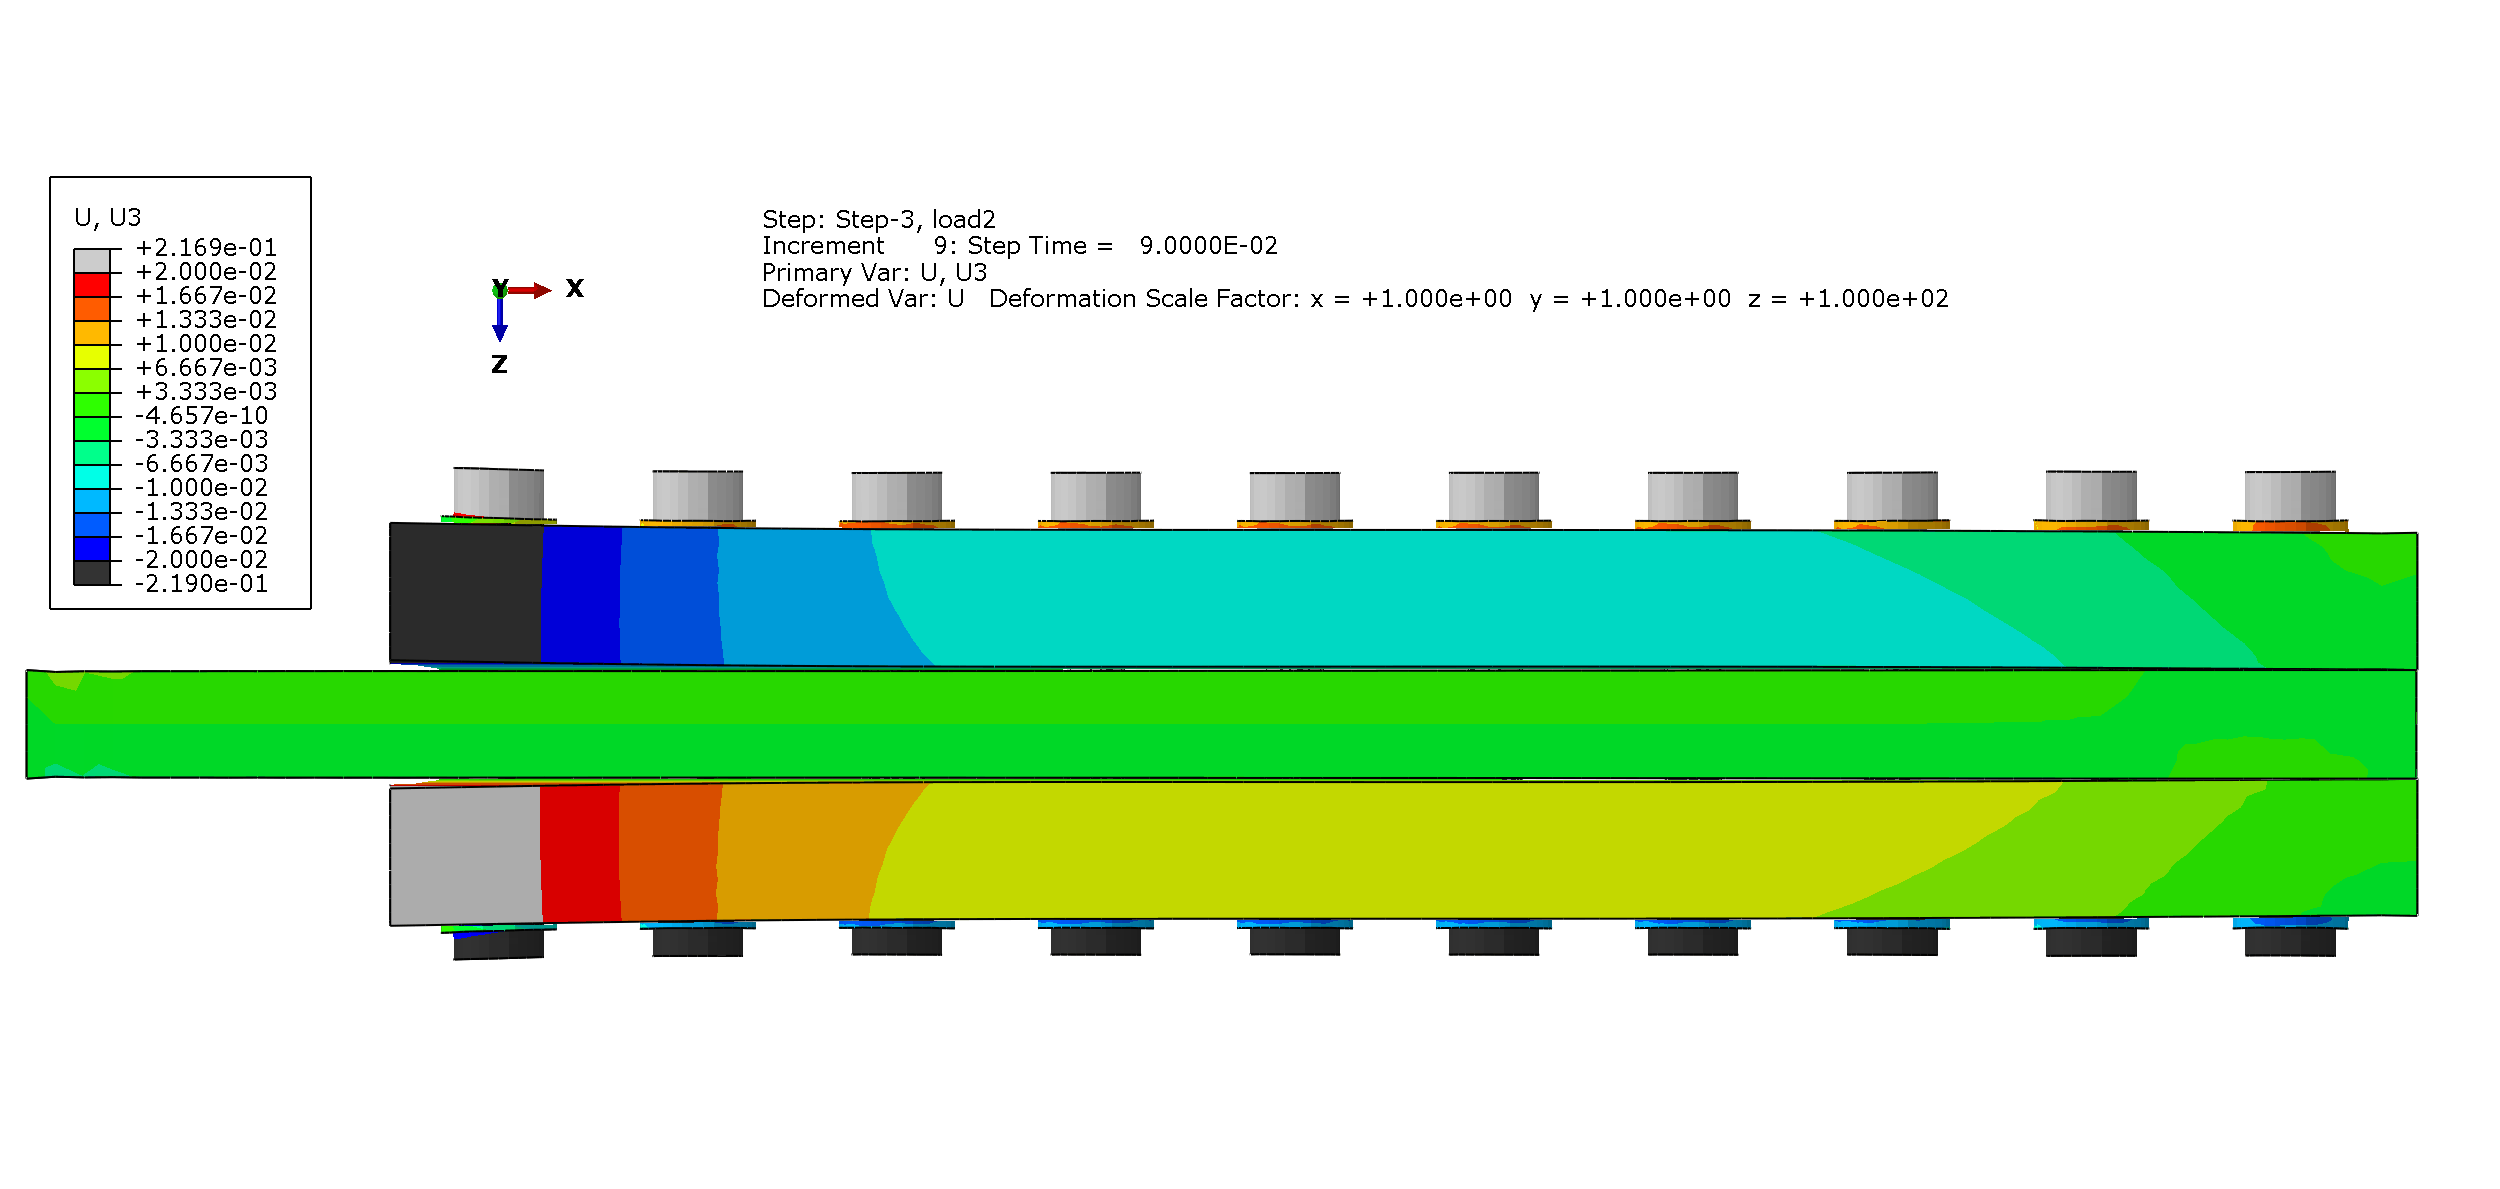
\includegraphics[width=0.8\textwidth]{imgs/ch7/U3-vfst.png}
%     \caption{Deformation of Z (U3) direction counter when load is 1384 kN}
%     \label{fig-u3vfst}
% \end{figure}


% Fig. \ref{fig-bcsche} shows the Boundary conditions and deformation schematic, The cross-sectional force acting on the main plate is divided into the cross-sectional forces of the main plate and splice plate via the shear transmit on the bolt. Assuming that the point of action of each cross-sectional force is at the center of the plate, an additional bending moment is generated in the bolt due to the eccentricity of the cross-sectional forces. The boundary condition at the end of the connection plate is free, so there is a tendency to deform outward toward the main plate faying surface when subjected to additional bending moments, resulting in a separation of the connection plate from the main plate, and therefore a loss of friction force.

% \begin{figure}[htbp]
%     \centering
%     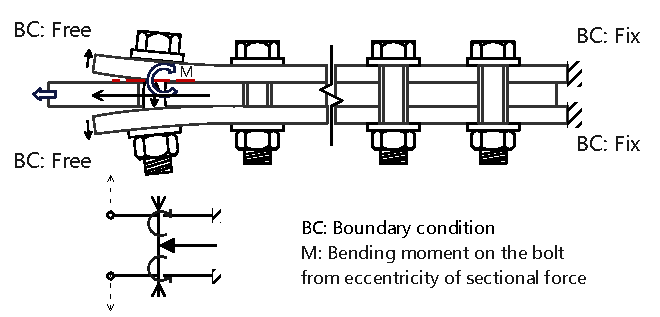
\includegraphics[width=0.9\textwidth]{imgs/ch7/bcschema.pdf}
%     \caption{Schematic of the boundary conditions and deformation}
%     \label{fig-bcsche}
% \end{figure}


% \subsubsection{Reduction factor for unevenly load sharing}

% Uneven load distribution in a bearing connection can cause a particular fastener to reach the specified strength before another, the load distribution can be seen in Fig. \ref{fig-bshare} in Chapter \ref{ch5}. In addition, due to the decrease in friction in a bearing connection, it returns to share more bearing pressure than expected, which can cause this fastener to reach a yield state more quickly. Based on the data from the FE analysis in Chapter \ref{ch5}, the correction factor due to the load sharing $\beta_{ls}$ is taken to be 0.9.

% Fig. \ref{fig-beals-b4} shows the distribution of bearing forces on individual bolts for this analysis (when the shear gross section of the bolt shaft yields, i.e., 1384 kN), and again it can be seen that the fasteners are not uniformly stressed.

% \begin{figure}[htbp]
%     \centering
%     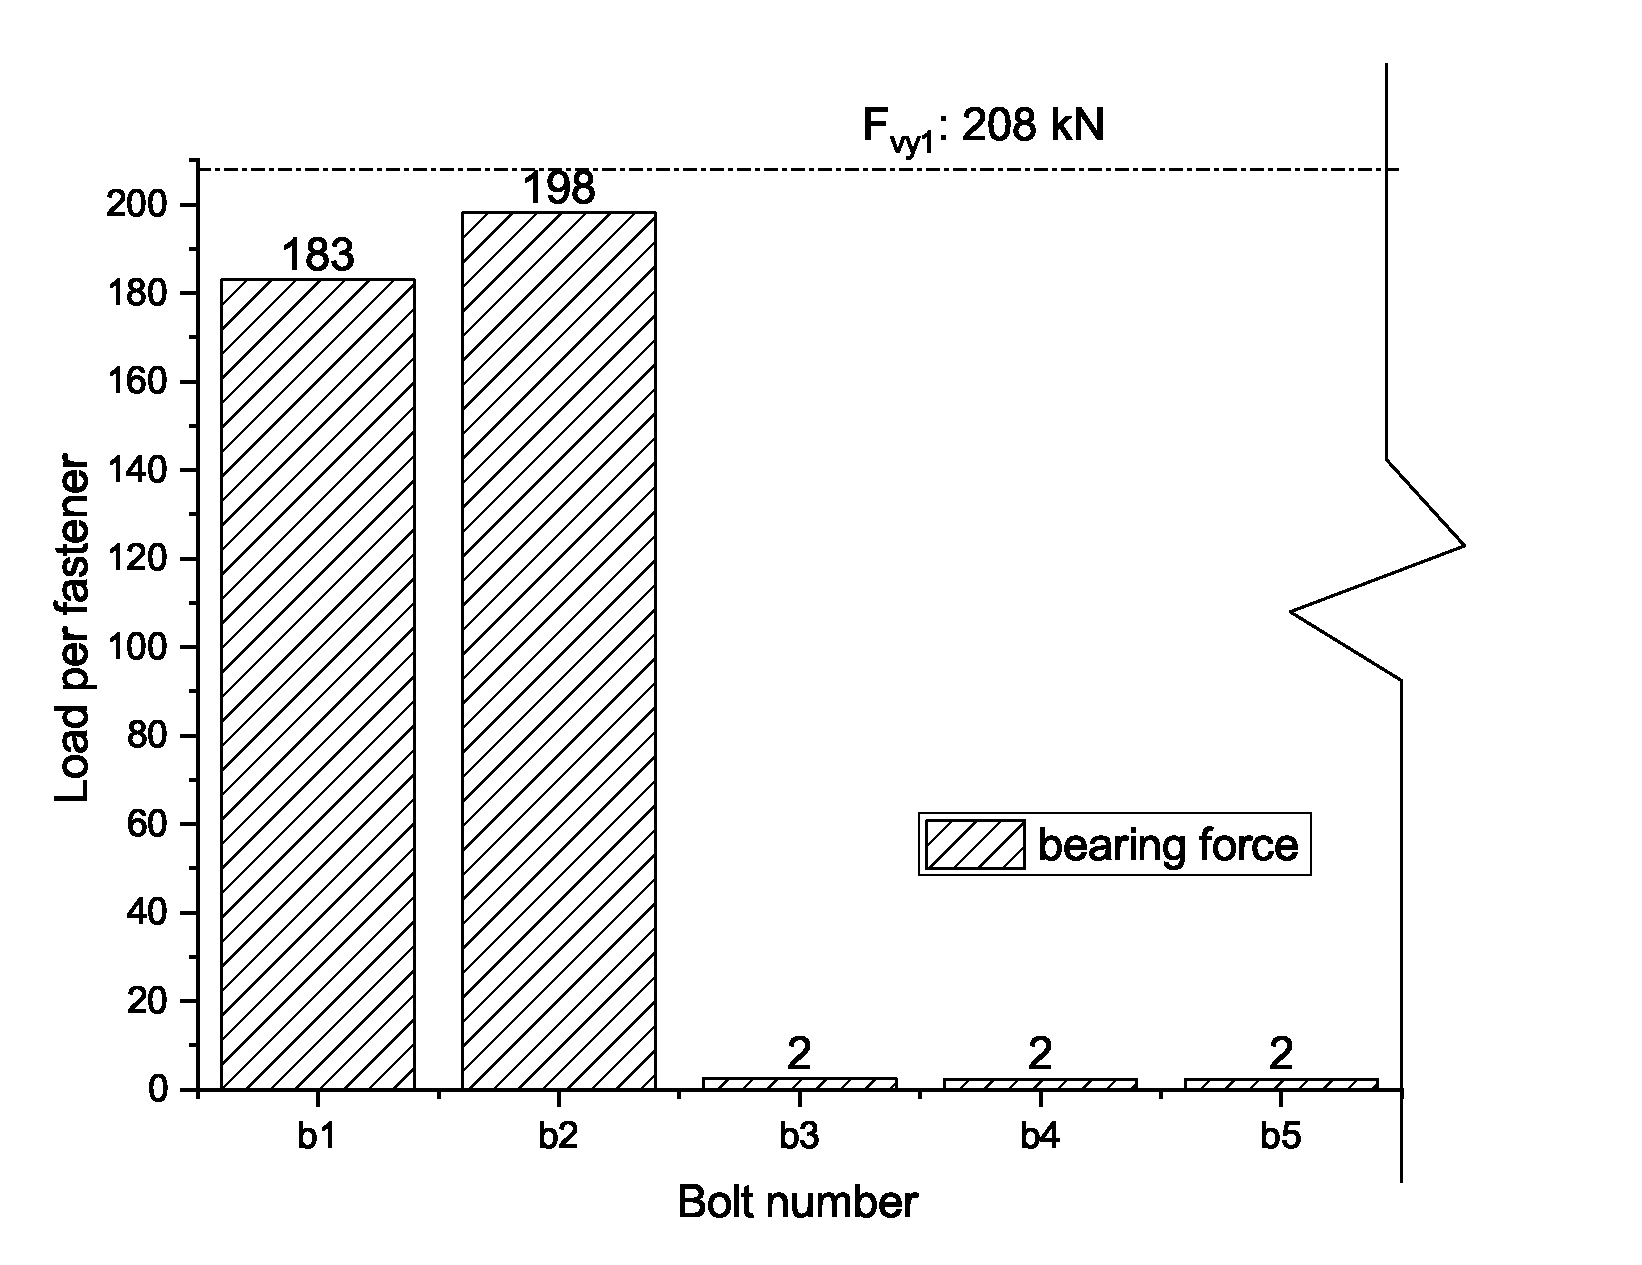
\includegraphics[width=0.7\textwidth]{imgs/ch7/beals-b4.eps}
%     \caption{the distribution of bearing forces on individual bolts for this analysis (when the shear gross section of the bolt shaft yields, i.e., 1384 kN)}
%     \label{fig-beals-b4}
% \end{figure}

% In addition, fasteners at the ends are always more affected by deformation than those measured internally due to the difference in boundary conditions. That is, at the front end of the joint, the connection plate is free while the main plate is fixed, so when loaded, the connection plate will always have a tendency to bend outward toward the face, which will exacerbate the deformation of the bolt. Therefore, this is one of the reasons for the uneven force on the end bolts.


% \subsubsection{Summary}

% For the shear yield strength of bolts, since the preload is significantly reduced when the shear surface of the bolt is plastically expanded, the immediate effect is the loss of the friction it bears, which can result in a reduction in friction $\alpha_{v}$. In addition, for the hybrid connection configured with bearing type connection at the end only, the bearing type connection at the end is affected by the uneven load distribution, the bolt subjected to more force is 1.2 times higher than the bolt subjected to less force, so for the sake of convenience of calculation, $\beta_{ls} = 0.9 $ is taken as the phenomenon of individual bolts subjected to too much load due to the uneven distribution of the load, which leads to the phenomenon of yield first, and this is also valid for the bearing yielding state.

% In addition, if there is a fastener for bearing type connection located at the front end, its friction will cause deformation of the main plate due to bending moment generated by shear, which will result in the loss of friction, so it is recommended that the friction of the front end (b1) bolt be ignored in such cases.

% For SLS :
% if bearing type connection is arranged at the front end of the joint :

% \begin{equation}
% \begin{aligned}
%     F_{hv} &= (n_f+ \alpha_v(n_b-1)) F_s + \beta_{ls} n_b F_{vy1} \\
%            &= (n_f + 0.7(n_b-1)) F_{s1} + 0.9 n_b F_{vy1}
% \end{aligned}
% \end{equation}

% if not:

% \begin{equation}
% \begin{aligned}
%     F_{hv} &= (n_f+ \alpha_v n_b) F_s + \beta_{ls} n_b F_{vy1} \\
%            &= (n_f + 0.7 n_b) F_{s1} + 0.9 n_b F_{vy1}
% \end{aligned}
% \end{equation}

% Summarizing with the above discussion, the two complementary coefficients can be respectively $\alpha_v = 0.75 \approx 0.7$, $\beta_{ls} = 0.9$

% For the maximum resistance due to bolt shear, although there will always be residual friction that will participate in the transfer of the load together until the maximum load is reached, however, since this is considered unreliable, the friction due to the preloading of the bolt is usually not taken into account in the calculation of the ultimate resistance. The same is true for hybrid joints, so for the design of the ultimate shear strength of hybrid joints, the calculation is normalized according to the following equation.

% For ULS:

% % \begin{equation}
% %     F_v = \beta_{ls} n A_s f_{ub}
% % \end{equation}
% \begin{equation}
%     F_v = n A_s f_{ub}
% \end{equation}

% \subsection{Bearing yield of the main plate}

% Hybrid connection bearing yielding mainly confirms the fastener holes of the bearing type connection, in Chapter \ref{ch4} mainly discusses the judgment of bearing yielding, for any fastener holes around the hole including to the direction of the plate thickness has reached the equivalent diameter range of the plastic region, the judgment of fastener holes bearing yielding occurs. Specific judgment can be referred to in Chapter \ref{ch4}, followed by a simple use of stress maps to describe the stress characteristics of bearing yielding.

% Table \ref{tabfe-beafst} lists the geometric information for this resolved case as well as the material and contact properties used. Table \ref{tabjr-bfst} lists the calculated resistance of the hybrid joints.

% \begin{table}[htbp]
% \centering
% \caption{Various property for FE analysis}\label{tabfe-beafst}
% \begin{tabular}{@{}cccccccccc@{}}
% \toprule
%  &
%   \begin{tabular}[c]{@{}c@{}}$w$\\ {[}mm{]}\end{tabular} &
%   \begin{tabular}[c]{@{}c@{}}$t$\\ {[}mm{]}\end{tabular} &
%   \begin{tabular}[c]{@{}c@{}}$d_0$\\ {[}mm{]}\end{tabular} &
%   \begin{tabular}[c]{@{}c@{}}Number of\\ bolt\end{tabular} &
%   \begin{tabular}[c]{@{}c@{}}Bolt for \\ bearing\end{tabular} &
%   $\mu$ &
%   \begin{tabular}[c]{@{}c@{}}$N_0$\\ {[}kN{]}\end{tabular} &
%   \begin{tabular}[c]{@{}c@{}}$f_y$\\ {[}Mpa{]}\end{tabular} &
%   \begin{tabular}[c]{@{}c@{}}$f_u$\\ {[}Mpa{]}\end{tabular} \\ \midrule
% shear-fst &  270 &  30 &  18 &  10 &  4 &  0.4 &  106 &  235 &  490 \\ \bottomrule
% \end{tabular}
% \end{table}


% \begin{table}[htbp]
% \centering
% \caption{Summary of joint resistance (unit: kN)}\label{tabjr-bfst}
% \begin{tabular}{@{}ccccccccc@{}}
% \toprule
%  &
%   \multicolumn{5}{c|}{SLS} &
%   \multicolumn{3}{c}{ULS} \\ \midrule
%  &
%   \begin{tabular}[c]{@{}c@{}}$F_s$\end{tabular} &
%   \begin{tabular}[c]{@{}c@{}}$F_{by}$ \end{tabular} &
%   \begin{tabular}[c]{@{}c@{}}$F_{vfy}$ \end{tabular} &
%   \begin{tabular}[c]{@{}c@{}}$F_h$ \end{tabular} &
%   \multicolumn{1}{c|}{\begin{tabular}[c]{@{}c@{}}$F_y$ \end{tabular}} &
%   \begin{tabular}[c]{@{}c@{}}$F_b$ \end{tabular} &
%   \begin{tabular}[c]{@{}c@{}}$F_v$ \end{tabular} &
%   \begin{tabular}[c]{@{}c@{}}$F_u$ \end{tabular} \\ \cmidrule(l){2-9} 
% bearing yiled &  848 &  441.6 &  835 &  1160 &  1738 &  2352 &  2320 &  3719 \\ \bottomrule
% \end{tabular}
% \end{table}

% Fig. \ref{fig-beafst} shows the The relationship between load and relative displacement when bearing yield first case occurs. The blue dashed line represents the bearing yield resistance of the hybrid joint obtained by calculation equation, and the red triangle represents the load obtained in the analysis when yielding occurs around the fastener holes equivalent area. It can be found that the bearing yield resistance obtained by calculation and the load obtained in the analysis are similar, and they both occur at the stage when the curves are in the nonlinear transition. It can be assumed that the formula, as well as the analytical judgment of bearing yielding is appropriate.

% \begin{figure}[htbp]
%     \centering
%     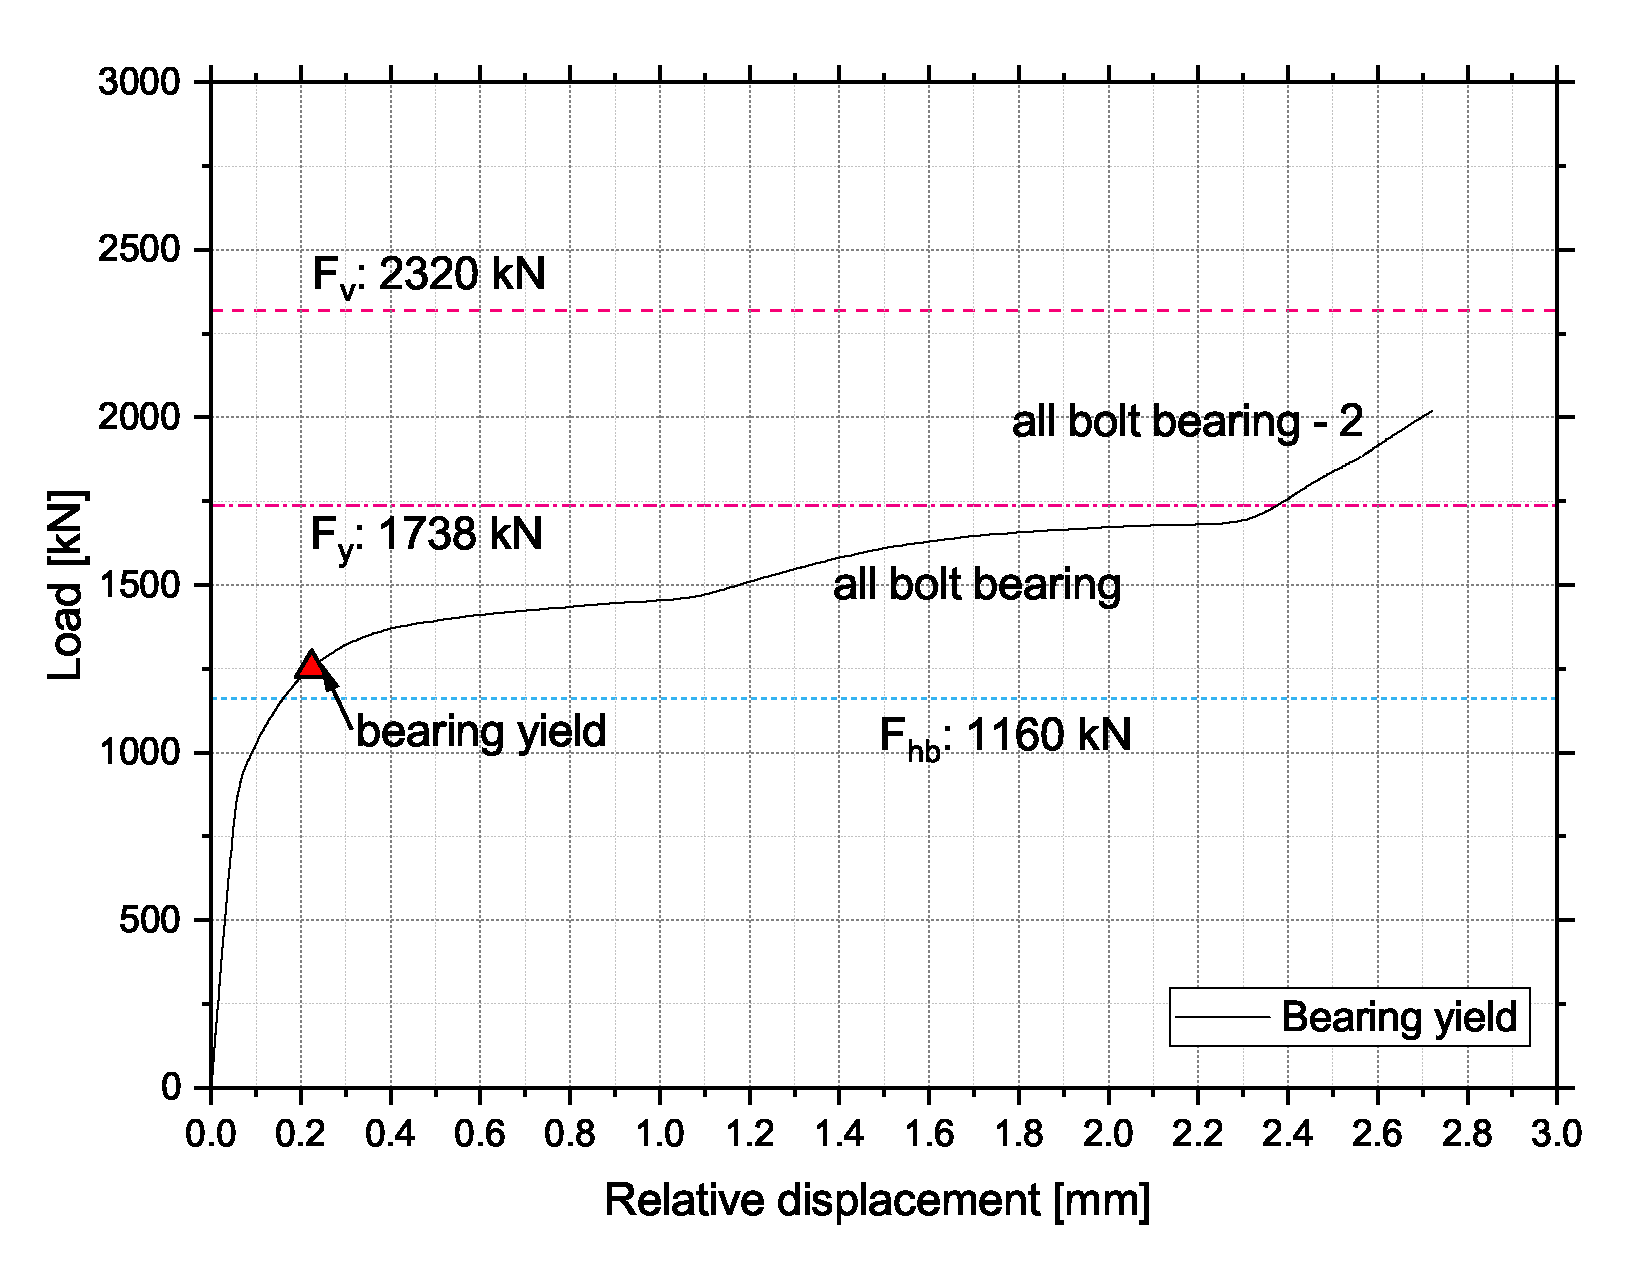
\includegraphics[width=0.7\textwidth]{imgs/ch7/b4s40t30.eps}
%     \caption{The relationship between load and relative displacement for bearing yield first case.}
%     \label{fig-beafst}
% \end{figure}

% Fig. \ref{fig-beafstcp} shows the Mises stress counter of the joint for bolts (thickness center of main plate, Maximum = 900 Mpa, when load = 1251 kN), Fig. \ref{fig-beafstcp-2} shows the Mises stress counter of the joint for the main plate (faying surface of the main plate, Maximum stress = 235 Mpa, when load = 1251 kN), From the figure, it can be found that when the load is equal to 1251 kN, the whole cross-section within the bearing contact range of the main plate has yielded, and it can be assumed that the joint has yielded under pressure, and at this time, the joint is in the limit state of yielding under pressure, and with reference to Fig. \ref{fig-beafst}, it can be found that the curve is experiencing a nonlinear change at this time, and it is about to enter into the stage of plastic ductility.

% Fig. \ref{fig-beafstcp} shows the Mises stress counter of the joint for the plate (thickness center of main plate, Maximum stress = 900 Mpa, when load = 1251 kN). Against Fig. \ref{fig-beafst}, it can be seen from this figure that it is not the yielding of the shear plane of the bolt that causes the curve to go into a nonlinear behavior, so this state can be ruled out.

% \begin{figure}[htbp]
%     \centering
%     \begin{minipage}[t]{0.8\textwidth}
%     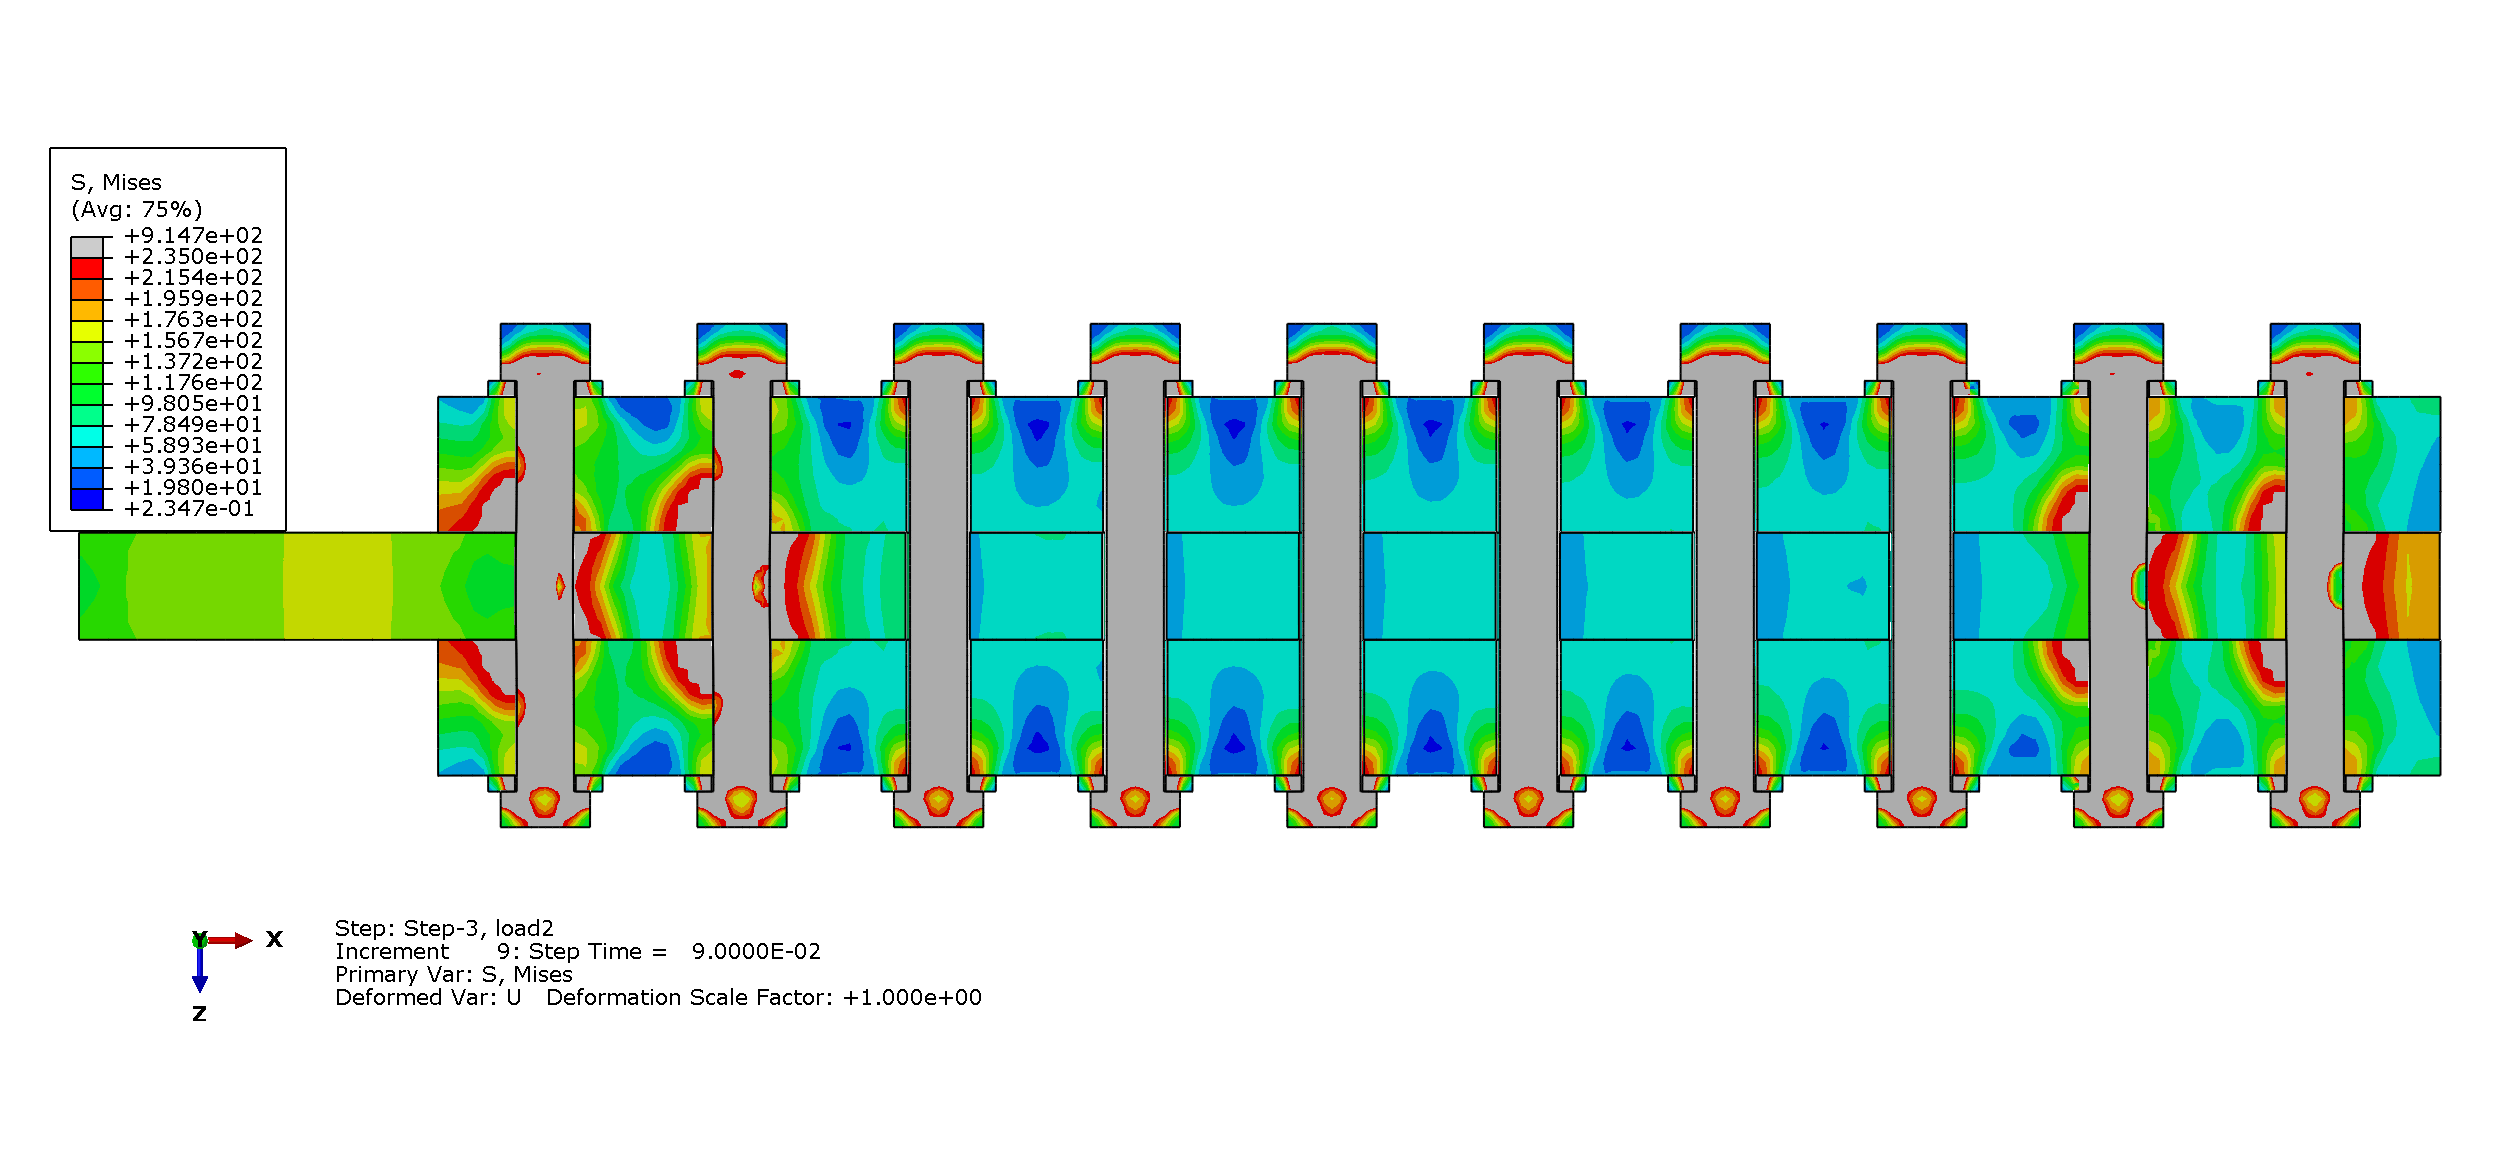
\includegraphics[width=\linewidth]{imgs/ch7/beafst-count-p.png}
%     \caption{Mises stress counter of the joint for bolts (thickness center of main plate, Maximum stress = 235 Mpa, when load = 1251 kN)}
%     \label{fig-beafstcp}
%     \end{minipage}
%     \begin{minipage}[t]{0.8\textwidth}
%     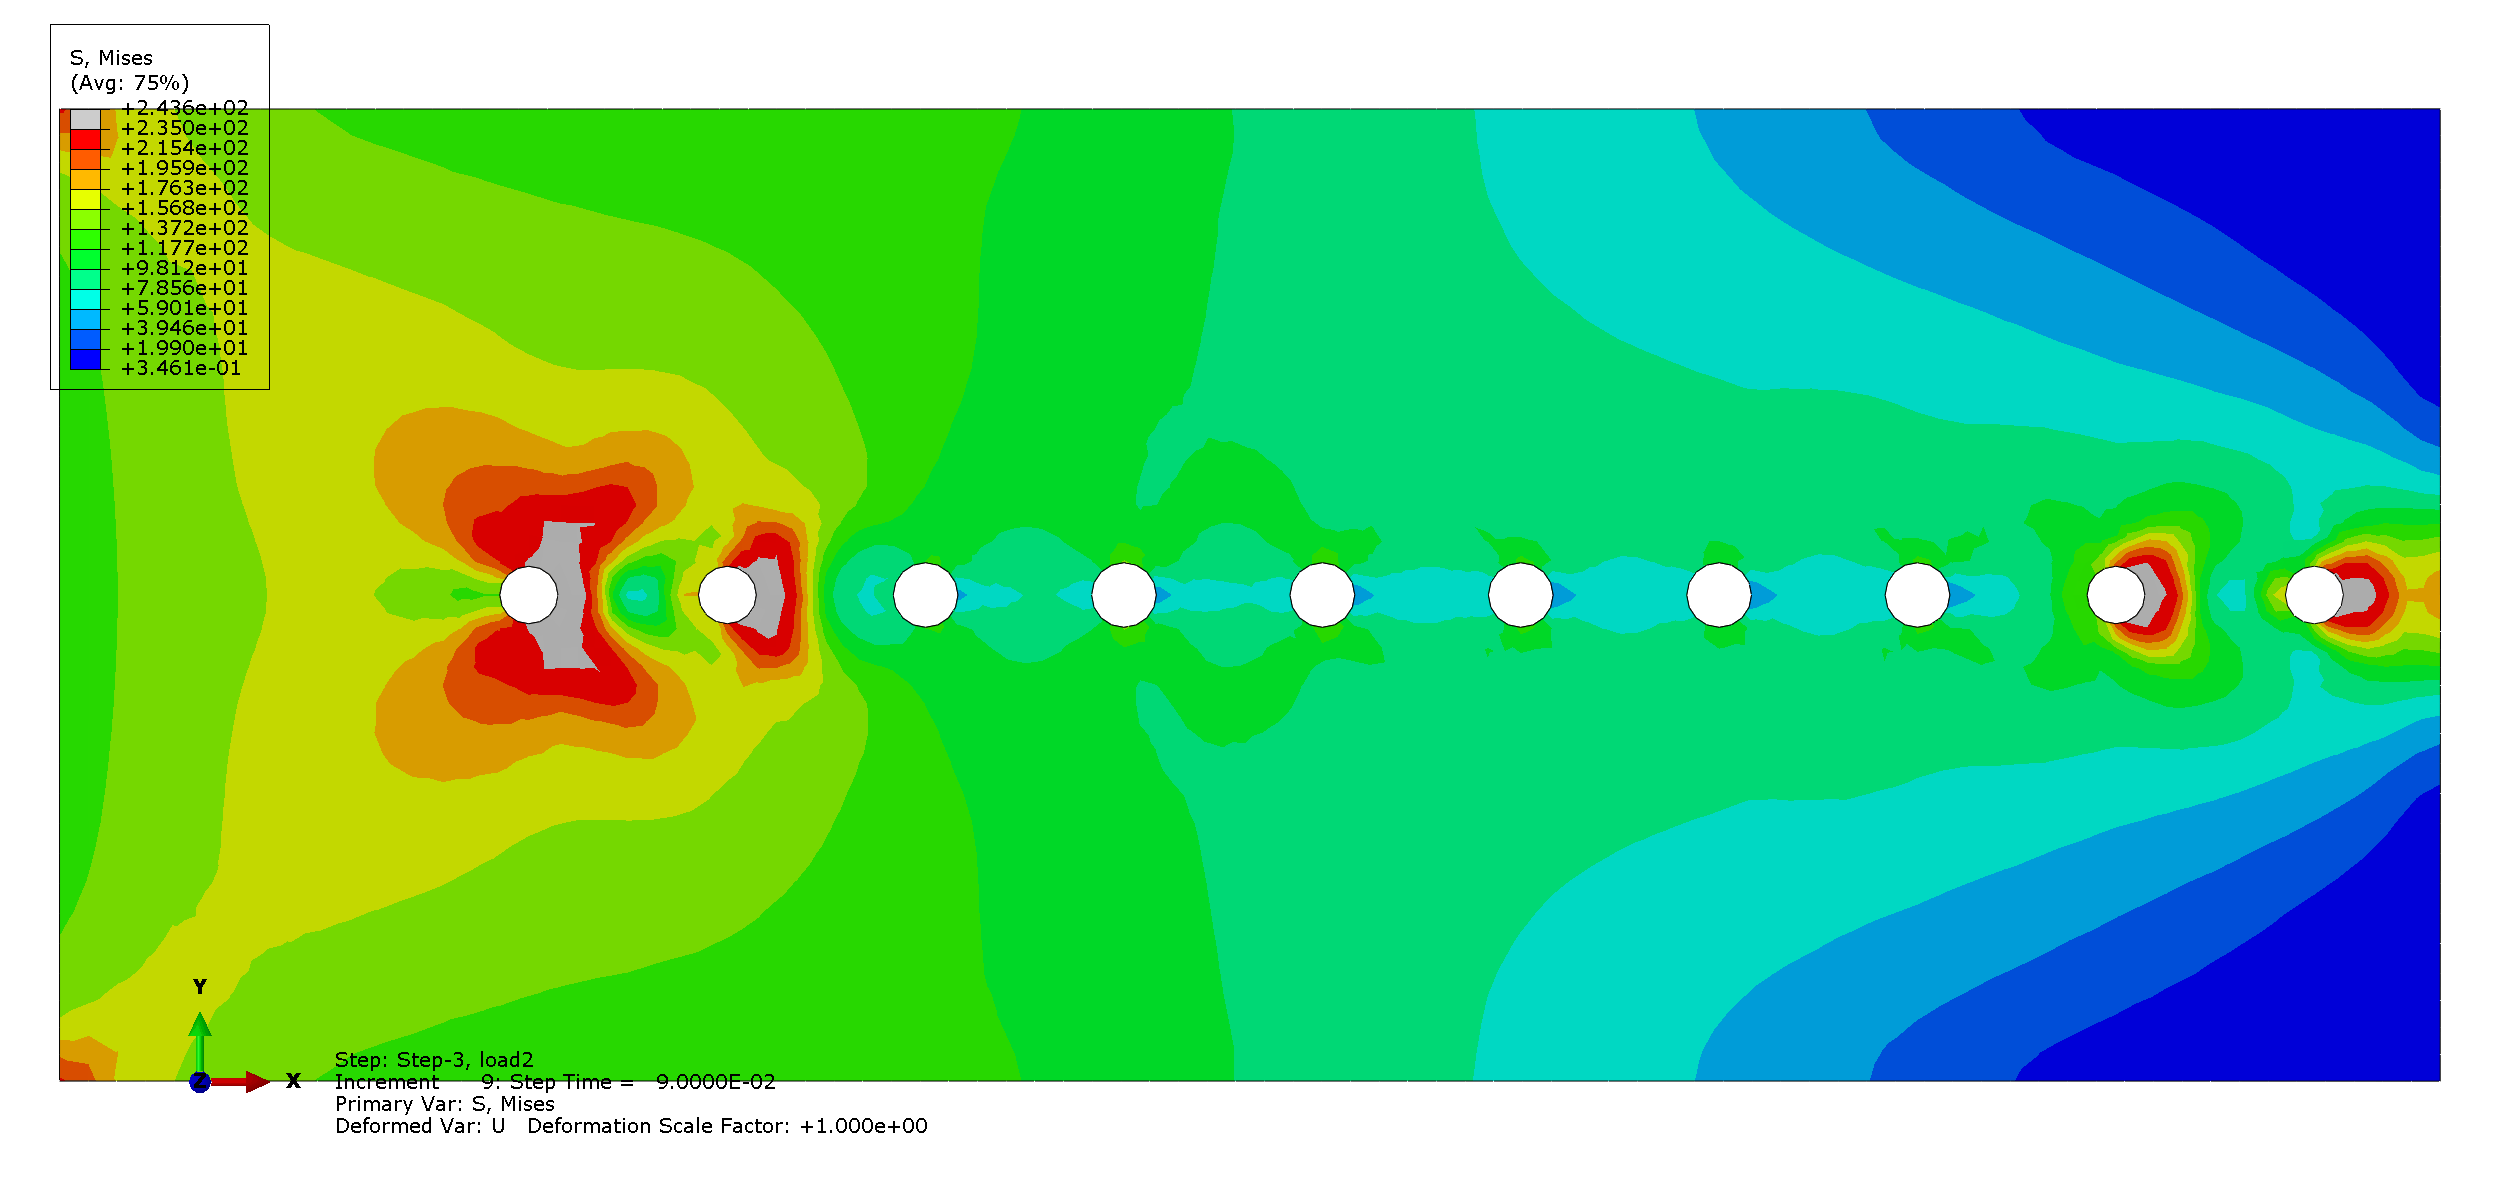
\includegraphics[width=\linewidth]{imgs/ch7/beafst-scout-mp.png}
%     \caption{Mises stress counter of the joint for the main plate (faying surface of the main plate, Maximum stress = 235 Mpa, when load = 1251 kN)}
%     \label{fig-beafstcp-2}
%     \end{minipage}
%     \begin{minipage}[t]{0.8\textwidth}
%     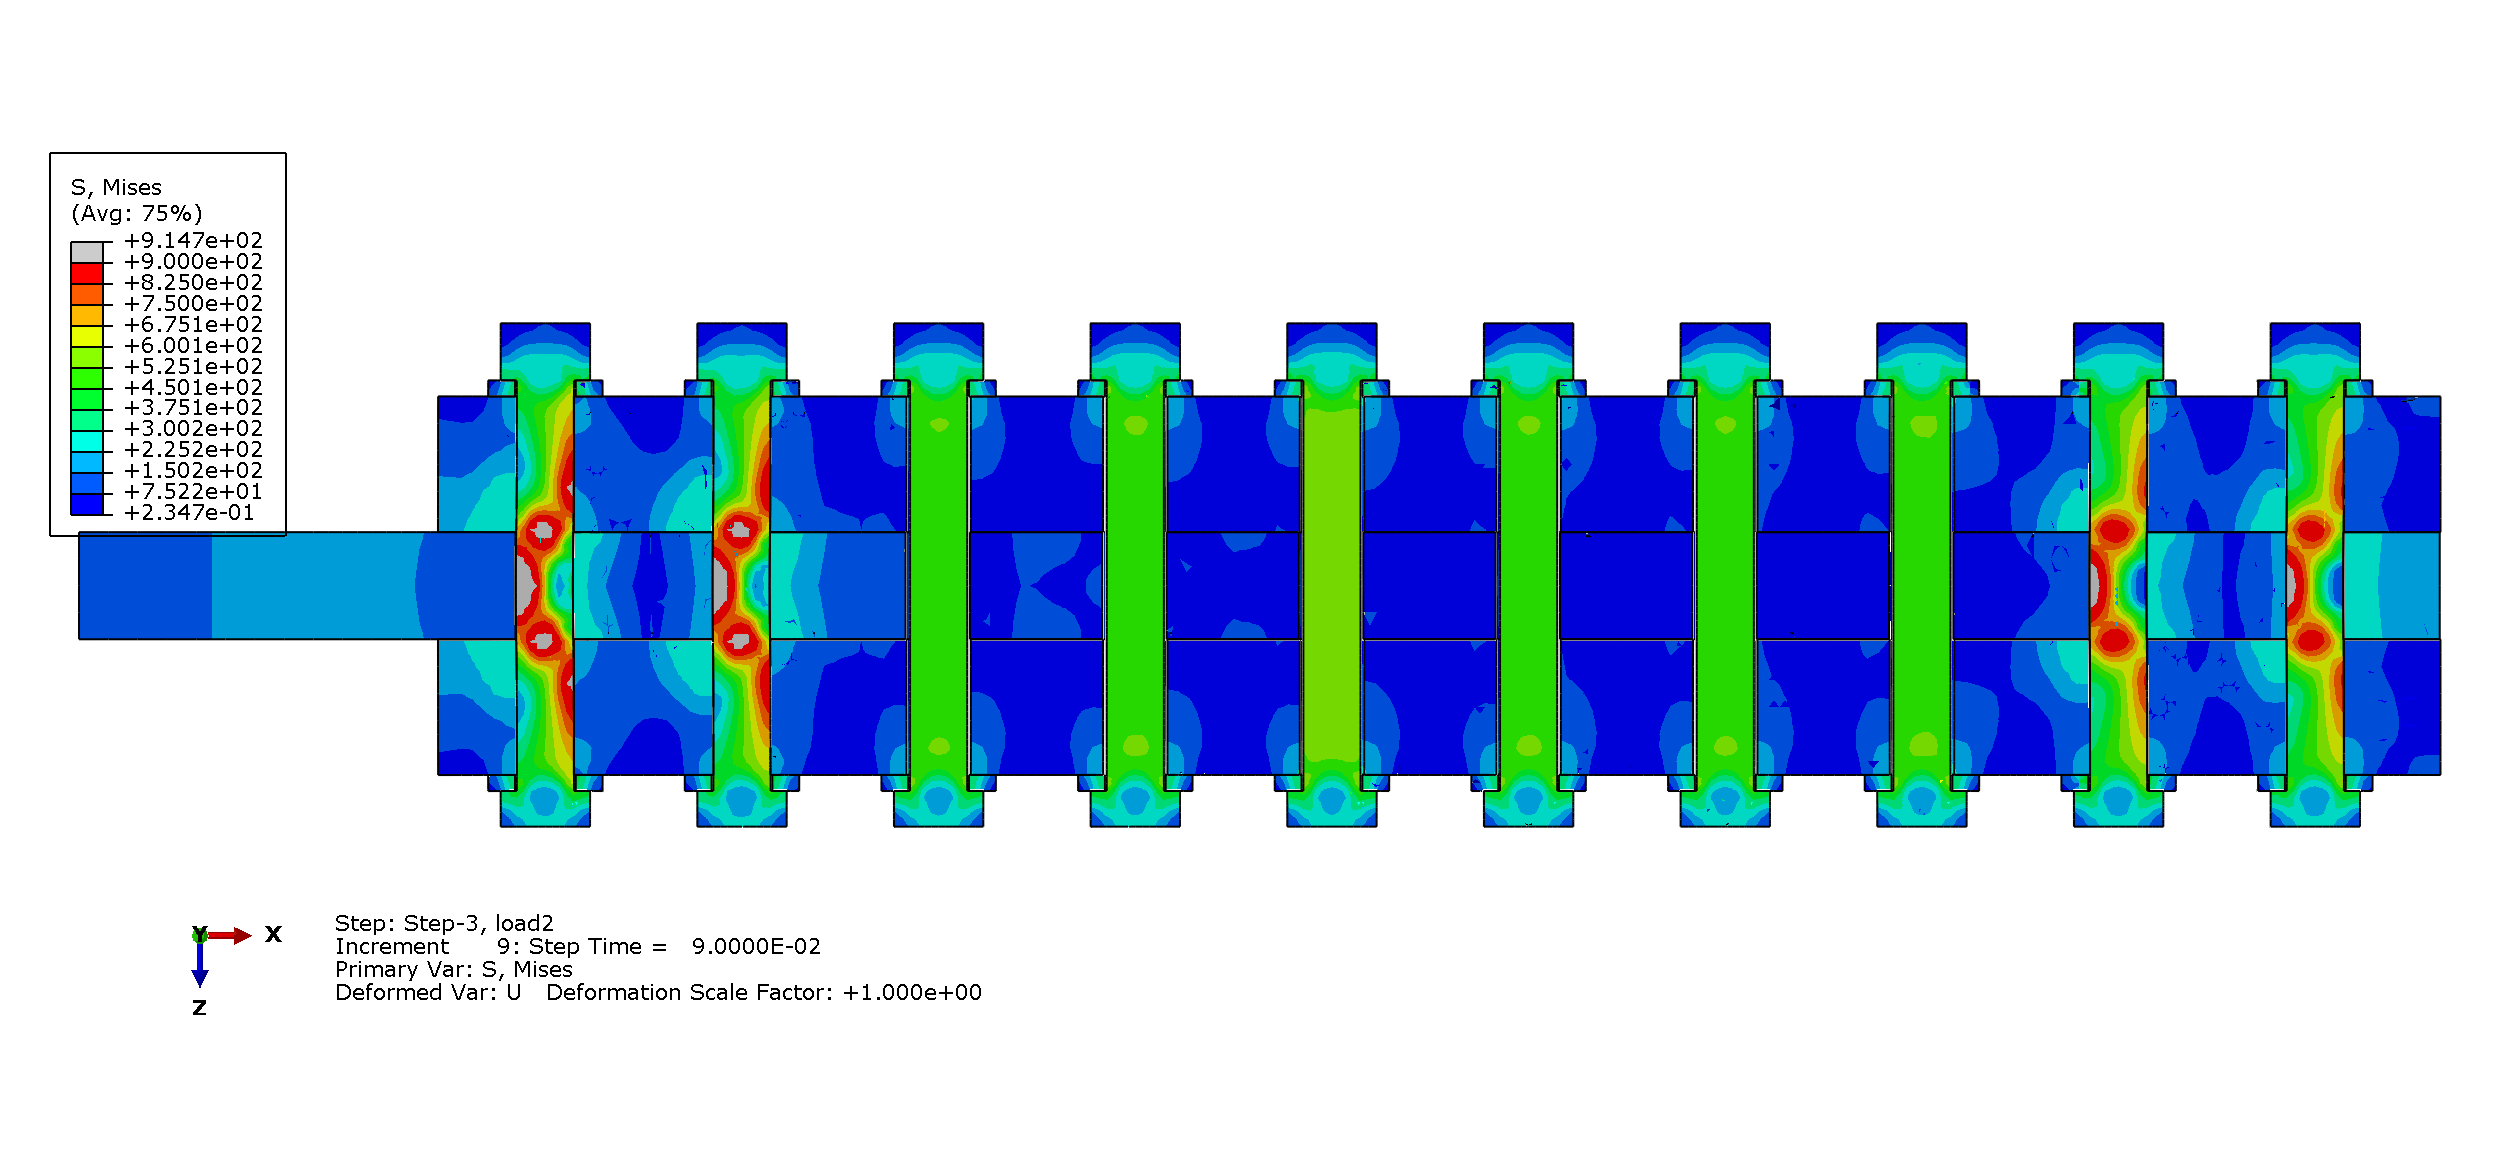
\includegraphics[width=\linewidth]{imgs/ch7/beafst-count-b.png}
%     \caption{Mises stress counter of the joint for the plate (thickness center of main plate, Maximum stress = 900 Mpa, when load = 1251 kN)}
%     \label{fig-beafstcb}
%     \end{minipage}
%     \label{fig-beafstc}
% \end{figure}



% \subsubsection{Reduction factor}

% Fig. \ref{fig-beafstls} shows the Decline ratio of bolt preload when load is equal to the 1251 kN (bearing yield first case). From the figure, it can be seen that when it is judged as bearing yielding, since the nonlinear behavior of the joint arises around the bolt holes of the main plate, there is not much effect on the shaft of the bolt, and the bolt shaft as a whole is still in the linear elasticity stage, so the preload of the bolt does not change significantly as in the case of shear yielding case. Although the preload still drops to about 0.9, this value is very small for the whole, so it is considered here that the correction factor for the slip strength regarding the preload can be disregarded for the bearing resistance yield case.

% \begin{figure}[htbp]
%     \centering
%     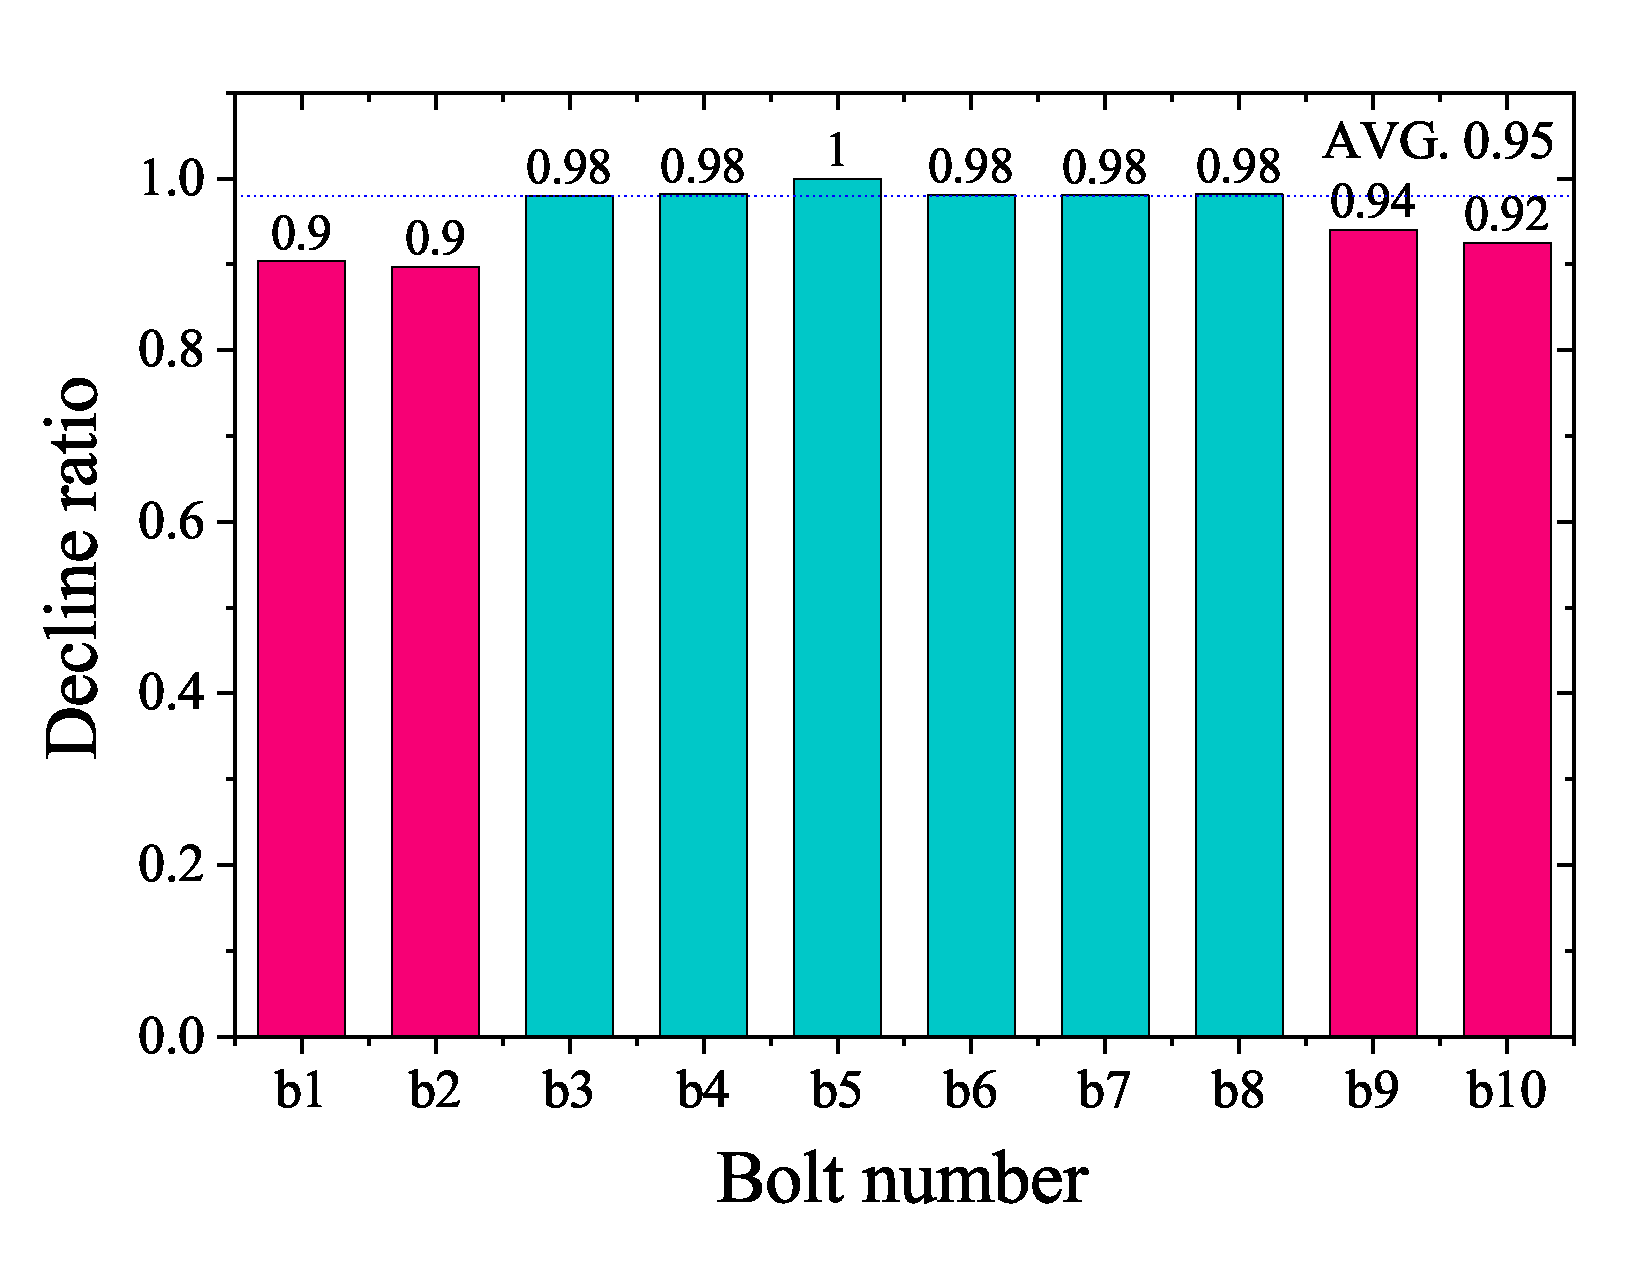
\includegraphics[width=0.7\textwidth]{imgs/ch7/b4t30w27-ls.eps}
%     \caption{Decline ratio of bolt preload when load is equal to the 1251 kN (bearing yield first case)}
%     \label{fig-beafstls}
% \end{figure}


% \subsubsection{Summary}

% For the bearing yield limit state, since the occurrence of nonlinear behavior depends around the main plate fastener holes, the fasteners used for bearing connections are also not subjected to excessive shear resulting in a loss of preload, however, like the shear yield mode, the friction located in the if the front end is configured with a fastener used for a bearing type of connection, which produces a moment due to shear, will cause the main plate to deform and will still result in a friction force Therefore, it is not recommended to take into account the friction of bolt (b1) at the front end for such cases. The reduction factor due to the uneven distribution of loads in the bearing connection is still applicable to bearing resistance, therefore it is still recommended to multiply this reduction factor $\beta_{ls}$ when calculating the bearing yield resistance $F_{hv}$.

% For SLS:
% if bearing type connection is arranged at the front end of the joint :

% \begin{equation}
% \begin{aligned}
%     F_{hb} &= (n-1) F_s + \beta_{ls} n_b F_{by1}\\
%            &= (n-1) F_s + 0.9 n_b F_{by1}
% \end{aligned}
% \end{equation}

% if not :

% \begin{equation}
% \begin{aligned}
%     F_{hb} &= n F_s + \beta_{ls} n_b F_{by1}\\
%            &= n F_s + 0.9 n_b F_{by1}
% \end{aligned}
% \end{equation}

% For ULS, see other specifications such as Eurocode 3:

% \begin{equation}
%     F_v = n k_m \alpha_b d t f_{u}
% \end{equation}


% \subsection{Net cross-section yield}

% For the net interfacial yield strength of the main slab, the method of calculation has not changed from the recommendations given in the various codes and is calculated according to the following equation.

% \begin{equation}
%     F_y = (w-d_0) t f_y
% \end{equation}



% \subsection{Design methods}




% For hybrid joints with friction and bearing connections, the service limit states can be categorized as: a.Shear yield limit state for the fastener shaft, b. Bearing yield limit state for main plate, c. Net cross-section yield limit state as shown in Fig. \ref{fig-schehysls}.

% \begin{figure}[htbp]
%     \centering
%     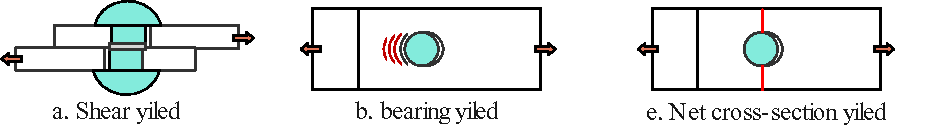
\includegraphics{imgs/ch7/sche-hy-sls.pdf}
%     \caption{Schematic of the yield mode on the serviceability limit state}
%     \label{fig-schehysls}
% \end{figure}

% Table\ref{tab-sumeq} summarizes the calculate equation for the hybrid joint on the serviceabilit limit state.

% Hybrid joints mainly take into account the loss of preload due to shearing of the fasteners and the loss of friction of the fasteners located at the ends, in addition to the proposed discount factor due to the uneven distribution of loads in the bearing connection.

% \begin{table}[htbp]
% \centering
% \caption{Calculate equation for hybrid joint on the SLS} \label{tab-sumeq}
% \begin{tabular}{@{}lcc@{}}
% \toprule
% \multicolumn{3}{c}{Serviceability limit state}                                                  \\ \midrule
% \multicolumn{1}{c}{} & \begin{tabular}[c]{@{}c@{}}If b1 arranged \\ fastener for bearing\end{tabular} & \begin{tabular}[c]{@{}c@{}}If \\ not\end{tabular} \\ \cmidrule(l){2-3} 
% \begin{tabular}[c]{@{}l@{}}Shear yield resistance\\ for fastener shaft $F_{hv}$\end{tabular} &$(n_f+ \alpha_v(n_b-1)) F_s + \beta_{ls} n_b F_{vy1}$ & $(n_f+ \alpha_v n_b) F_s + \beta_{ls} n_b F_{vy1}$ \\
% \begin{tabular}[c]{@{}l@{}}Bearing yield resistance\\ for main plate $F_{hb}$ \end{tabular}   & $(n-1) F_s + \beta_{ls} n_b F_{by1}$ & $ n F_s + \beta_{ls} n_b F_{by1}$ \\
% \begin{tabular}[c]{@{}l@{}}Net cross-section yield\\ resistance $F_y$\end{tabular}   & \multicolumn{2}{c}{$ (w-d_0) t f_y$} \\ \bottomrule
% \end{tabular}
% \end{table}

% Where, $\alpha_v$ is Correction factor for loss of preload due to shear failure, $\beta_{ls}$ is the correction factor for load sharing. $n$ is the number of the fastener, $n_f$ is the number of the fastener for friction type connections, $n_b$ is the number of the fastener for bearing type connections, $F_{by1}= dtf_y$, $F_{vy1} = A_s f_{yb}/\sqrt{3}$.

% In addition, the reduction factor due to the conversion of static friction to kinetic friction should also be considered. However, the loading rate required for the conversion of static friction to kinetic friction varies according to the joint processing conditions, so in order to simplify the calculations, the friction coefficient can be considered as a factor of slip instead of slip coefficient for calculating the slip strength, and this topic will be discussed in the future to calculate the reliability of the calculation based on the coefficient of friction.

% For the limit states, it is considered sufficient to follow the existing methods of strength calculation and classification. The only difference is that since all fasteners do not enter the bearing connection at the same time, fasteners that enter the bearing connection at the beginning may fail prematurely due to early entry into the bearing state, and therefore the strength of the limit states of the hybrid connection may be considered to require a reduction factor.


\section{Conclusions}

This chapter focused on the mechanical behavior of hybrid connections, emphasizing deformation, load sharing, and the interaction of bearing and friction mechanisms.


\subsubsection*{Deformation behavior}


 In the case of the bolt shank shear yield limit state, the hybrid joints arranged with two and four fitted bolts (see Figure \ref{fig-loadrd-beaf}) produce almost the same relative displacements of approximately 0.4 $mm$ when the bolt shank shear yield strength $P_{h,sh}$ is reached. 
    
%ボルトシャンク全体せん断降伏限界状態の場合、2本の支圧型ボルト(図\ref{fig-ldoa2b}参照)と4本の支圧型ボルト(図\ref{fig-ldoa2b}参照)を配したハイブリッド継手では、ボルトシャンク全体せん断降伏強度P_{h,sh}に達したときの相対変位はほぼ同じ0.43mmとなる。これは、ボルトがせん断面で降伏したときに生じる弾性変形量が同じであることによると考えられる。従って、判定条件をボルトシャンクのせん断降伏強度時の荷重とすれば、そのボルトで生じる弾性変形量は同一と仮定できる。

Although the relative displacement at E-10mm (the location 10 mm away from the inner side of the joint, see Figure \ref{rd-distri}) was approximately 0.4 mm when the hybrid joint was in SLS, the relative displacement distribution of the long hybrid joint is significantly uneven, with an overall mean of 0.24 mm and a median of 0.2 mm.
    

\subsubsection*{Load sharing and interaction mechanisms}

The fit bolts exhibit varying degrees of friction force degradation due to the different load transfer mechanisms of the bearing and friction, with the frontmost \# 1 bolt experiencing the most severe reduction. When four fitted bolts are used (two at each end), uneven bearing load distribution arises. Although the second \# 2 bolt appears to share a higher load, the frontmost \# 1 bolt relies almost entirely on the bearing to transfer the load due to the loss of friction force, resulting in the highest bearing force among all fitted bolts and leading to its bolt shank shear yielding first. Moreover, the uneven bearing load distribution prevents the bearing resistance from reaching the design bearing strength.

%長いすべり型継手の場合、荷重分布の偏りにより中央のボルトが許容すべり値を超えて設計すべり強度に達することができず、日本の道路橋示方書によってすべり耐力の低減係数が提案されている。一方、ハイブリッド継手では、すべり型継手の中央ボルトでは一様な荷重分担が生じ、設計すべり耐力に達する。一方、支圧型のボルトでは支圧伝達機構のため種々の程度の摩擦力劣化が生じ、最前列の#1ボルトで最も厳しい低減が生じる。4本の支圧型ボルト(各端部2本)を使用する場合、支圧荷重分布の偏りが生じる。#2ボルトが比較的高い荷重を分担するように見えるが、#1ボルトはほとんど全荷重を支圧で伝達せざるを得ず、摩擦力を失っているため、全支圧型ボルトの中で最大の支圧力が作用し、これがボルトシャンクの全体耐力に先行して降伏する。さらに、支圧荷重の偏り分布により、支圧耐力が設計支圧強度に達することができない。


\subsubsection*{Interaction of bearing and friction}

The cross-sectional force acting on the main plate is divided into forces on the main and splice plates via bolt shear transfer, generating an additional bending moment in the bolt due to the eccentricity of these forces. The shear bending of the fit bolt causes a severe loss of preload, resulting in a significant reduction in the frictional force it can transmit.

In addition, this bending moment causes the free end of the splice plate to deform outwards from the main plate, with a relative displacement of 0.43 mm at E-10mm and a maximum out-of-plane deformation of 0.07 mm at the end when the connection reaches bolt shank shear yield, resulting in separation and a loss of friction force. 

During Stage 1 of the hybrid connection, the bearing connection experiences delayed loading (the bearing starts to transfer load after a certain amount of slip occurs). Additionally, since the uneven load distribution of the bearing force in the fit bolts and the loss of friction force in the front bolt \#1, bolt shank shear yield generally occurs first in the front bolt \#1, and the bearing force could not reach the strength corresponding to the number of bolts.

% %主板に作用する断面力は、ボルトのせん断伝達を介して主板と継手板の力に分配され、この力の偏心によりボルトに追加曲げモーメントが生じる。この曲げモーメントにより、継手板の自由端が主板の摩擦面から外側に変形し、離間と摩擦力の喪失が生じる。この追加曲げモーメントにより継手板は変形し、ボルトシャンク全体せん断降伏時にE-10mmで0.43mmの相対変位と、端部で0.07mmの最大面外変形が生じる。ボルトの圧縮側では、ボルト変形により高い接触圧が発生するが、全体として摩擦面の接触圧は低下傾向にある。


% %在混合阶段处于stage-1时,由于摩擦的高刚性,承压连接会出现延迟受力(承压会在产生一定的滑移量之后开始传递载荷),且由于fit螺栓承压力的载荷分担不均匀,以及前端 \# 1螺栓的摩擦力损失,螺栓剪切屈服一般会发生在前端的\# 1螺栓,承压力达不到螺栓数量的强度。
% %ハイブリッド継手の第1段階では、摩擦の高い剛性により、支圧継手部の荷重伝達が遅延する(すべりが生じた後に支圧荷重が伝達され始める)。加えて、支圧型ボルトの支圧力分布の偏りと最前列ボルト#1の摩擦力喪失により、通常、最前列ボルト#1でボルトシャンク全体せん断降伏が先行し、ボルト本数分の支圧強度に到達できない。

%\end{itemize}

\subsubsection*{Reduction factor of bearing and friction}


%本文提出在计算混合连接剪切屈服强度时,分别对摩擦力和承压力进行折减,可以通过公式20计算其强度。其中摩擦力的折减系数参考公式21,配置两根和4根fit螺栓的情况分别取不同的折减系数,而关于承压力的折减系数,由于其偏差较小,因此取此次解析结果的下99%CI值作为折减系数,为0.76(统计结果可以参考表1). 通过公式20校正后的计算结果与解析值也较为吻合(见图19-c)。
This study proposes separately reducing the friction force and bearing force when calculating the bolt shank shear yielding strength of a hybrid connection, and its strength can be calculated using Eq. \ref{eq-pvh-2}. For the reduction factor of the friction force, refer to Eq. \ref{eq-as}, where different reduction factors are taken for the cases with two and four fitted bolts. As for the reduction factor of the bearing force, since its deviation is small, the lower 99\% CI of 0.76 from the analysis results in this study is taken as the reduction factor (the statistical results are listed in Table \ref{tab-rdfactor}). After correction using Eq. \ref{eq-pvh-2}, the calculated results match well with the analytical values (see Figure \ref{fig-fhv-cor2}).